% Judul dokumen
\title{Buku Tugas Akhir ITS}
\author{Musk, Elon Reeve}

% Pengaturan ukuran teks dan bentuk halaman dua sisi
\documentclass[12pt,twoside]{report}

% Pengaturan ukuran halaman dan margin
\usepackage[a4paper,top=30mm,left=30mm,right=20mm,bottom=25mm]{geometry}

% Pengaturan ukuran spasi
\usepackage[singlespacing]{setspace}

% Pengaturan detail pada file PDF
\usepackage[pdfauthor={\@author},bookmarksnumbered,pdfborder={0 0 0}]{hyperref}

% Pengaturan jenis karakter
\usepackage[utf8]{inputenc}

% Pengaturan pewarnaan
\usepackage[table,xcdraw]{xcolor}

% Pengaturan kutipan artikel
\usepackage[style=ieee, backend=biber]{biblatex}

% Package lainnya
\usepackage{changepage}
\usepackage{enumitem}
\usepackage{eso-pic}
\usepackage{txfonts} % Font times
\usepackage{etoolbox}
\usepackage{graphicx}
\usepackage{lipsum}
\usepackage{longtable}
\usepackage{tabularx}
\usepackage{wrapfig}
\usepackage{float}
\usepackage{booktabs}
\usepackage{subcaption}
\usepackage{graphicx}

% Definisi untuk "Hati ini sengaja dikosongkan"
\patchcmd{\cleardoublepage}{\hbox{}}{
  \thispagestyle{empty}
  \vspace*{\fill}
  \begin{center}\textit{[Halaman ini sengaja dikosongkan]}\end{center}
  \vfill}{}{}

% Pengaturan penomoran halaman
\usepackage{fancyhdr}
\fancyhf{}
\renewcommand{\headrulewidth}{0pt}
\pagestyle{fancy}
\fancyfoot[LE,RO]{\thepage}
\patchcmd{\chapter}{plain}{fancy}{}{}
\patchcmd{\chapter}{empty}{plain}{}{}

% Command untuk bulan
\newcommand{\MONTH}{%
  \ifcase\the\month
  \or Januari% 1
  \or Februari% 2
  \or Maret% 3
  \or April% 4
  \or Mei% 5
  \or Juni% 6
  \or Juli% 7
  \or Agustus% 8
  \or September% 9
  \or Oktober% 10
  \or November% 11
  \or Desember% 12
  \fi}
\newcommand{\ENGMONTH}{%
  \ifcase\the\month
  \or January% 1
  \or February% 2
  \or March% 3
  \or April% 4
  \or May% 5
  \or June% 6
  \or July% 7
  \or August% 8
  \or September% 9
  \or October% 10
  \or November% 11
  \or December% 12
  \fi}

% Pengaturan format judul bab
\usepackage{titlesec}
\titleformat{\chapter}[display]{\bfseries\Large}{BAB \centering\Roman{chapter}}{0ex}{\vspace{0ex}\centering}
\titleformat{\section}{\bfseries\large}{\MakeUppercase{\thesection}}{1ex}{\vspace{1ex}}
\titleformat{\subsection}{\bfseries\large}{\MakeUppercase{\thesubsection}}{1ex}{}
\titleformat{\subsubsection}{\bfseries\large}{\MakeUppercase{\thesubsubsection}}{1ex}{}
\titlespacing{\chapter}{0ex}{0ex}{4ex}
\titlespacing{\section}{0ex}{1ex}{0ex}
\titlespacing{\subsection}{0ex}{0.5ex}{0ex}
\titlespacing{\subsubsection}{0ex}{0.5ex}{0ex}

% Atur variabel berikut sesuai namanya

% nama
\newcommand{\name}{Arya Abdul Azis}
\newcommand{\authorname}{Azis, Arya Abdul}
\newcommand{\nickname}{Arya}
\newcommand{\advisor}{Mochamad Hariadi, S.T., M.Sc., Ph.D}
\newcommand{\coadvisor}{Reza Fuad Rachmadi, S.T., M.T., Ph.D}
\newcommand{\examinerone}{Dr. Galileo Galilei, S.T., M.Sc}
\newcommand{\examinertwo}{Friedrich Nietzsche, S.T., M.Sc}
\newcommand{\examinerthree}{Alan Turing, ST., MT}
\newcommand{\headofdepartment}{Dr. Supeno Mardi Susiki Nugroho,S.T.,M.T.}

% identitas
\newcommand{\nrp}{5024201069}
\newcommand{\advisornip}{199691209199703 1 002}
\newcommand{\coadvisornip}{19850403201212 1 001}
\newcommand{\examineronenip}{18560710 194301 1 001}
\newcommand{\examinertwonip}{18560710 194301 1 001}
\newcommand{\examinerthreenip}{18560710 194301 1 001}
\newcommand{\headofdepartmentnip}{19700313199512 1 001}

% judul
\newcommand{\tatitle}{INTEROPERABILITAS NFT BERBASIS BLOCKCHAIN MENGGUNAKAN SMART CONTRACT PADA WEB3.0}
\newcommand{\engtatitle}{\emph{BLOCKCHAIN-BASED NFT INTEROPERABILITY USING SMART
CONTRACTS IN WEB3.0}}

% tempat
\newcommand{\place}{Surabaya}

% jurusan
\newcommand{\studyprogram}{Teknik Komputer}
\newcommand{\engstudyprogram}{Computer Engineering}

% fakultas
\newcommand{\faculty}{Teknologi Elektro dan Informatika Cerdas}
\newcommand{\engfaculty}{Intelligent Electrical and Informatics Technology}

% singkatan fakultas
\newcommand{\facultyshort}{FTEIC}
\newcommand{\engfacultyshort}{FTEIC}

% departemen
\newcommand{\department}{Teknik Komputer}
\newcommand{\engdepartment}{Computer Engineering}

% kode mata kuliah
\newcommand{\coursecode}{EC234801}


% Tambahkan format tanda hubung yang benar di sini
\hyphenation{
  ro-ket
  me-ngem-bang-kan
  per-hi-tu-ngan
  tek-no-lo-gi
  me-la-ku-kan
  ber-so-si-al-i-sa-si
}

% Menambahkan resource daftar pustaka
\addbibresource{pustaka/pustaka.bib}

% Pengaturan format potongan kode
\usepackage{listings}
\definecolor{comment}{RGB}{0,128,0}
\definecolor{string}{RGB}{255,0,0}
\definecolor{keyword}{RGB}{0,0,255}
\lstdefinestyle{codestyle}{
  commentstyle=\color{comment},
  stringstyle=\color{string},
  keywordstyle=\color{keyword},
  basicstyle=\footnotesize\ttfamily,
  numbers=left,
  numberstyle=\tiny,
  numbersep=5pt,
  frame=lines,
  breaklines=true,
  prebreak=\raisebox{0ex}[0ex][0ex]{\ensuremath{\hookleftarrow}},
  showstringspaces=false,
  upquote=true,
  tabsize=2,
}
\lstset{style=codestyle}

% Isi keseluruhan dokumen
\begin{document}

% Sampul luar Bahasa Indonesia
\newcommand\covercontents{sampul/konten-id.tex}
\AddToShipoutPictureBG*{
  \AtPageLowerLeft{
    % Ubah nilai berikut jika posisi horizontal background tidak sesuai
    \hspace{-3.25mm}

    % Ubah nilai berikut jika posisi vertikal background tidak sesuai
    \raisebox{0mm}{
      
\includegraphics[width=\paperwidth,height=\paperheight]{sampul/gambar/sampul-luar.png}
    }
  }
}

% Menyembunyikan nomor halaman
\thispagestyle{empty}

% Pengaturan margin untuk menyesuaikan konten sampul
\newgeometry{
  top=55mm,
  left=30mm,
  right=20mm,
  bottom=20mm
}

\begin{flushleft}

  % Pemilihan font sans serif
  \sffamily

  % Pemilihan warna font putih
  \color{white}

  % Pemilihan font bold
  \fontseries{bx}
  \selectfont
  \begin{spacing}{1.5}
    \input{\covercontents}
  \end{spacing}

\end{flushleft}

\restoregeometry


% Atur ulang penomoran halaman
\setcounter{page}{1}

% Sampul dalam Bahasa Indonesia
\renewcommand\covercontents{sampul/konten-id.tex}
\AddToShipoutPictureBG*{
  \AtPageLowerLeft{
    % Ubah nilai berikut jika posisi horizontal background tidak sesuai
    \hspace{-4mm}

    % Ubah nilai berikut jika posisi vertikal background tidak sesuai
    \raisebox{0mm}{
      
\includegraphics[width=\paperwidth,height=\paperheight]{sampul/gambar/sampul-luar-tipis.png}
    }
  }
}

% Menyembunyikan nomor halaman
\thispagestyle{empty}

% Pengaturan margin untuk menyesuaikan konten sampul
\newgeometry{
  top=65mm,
  left=30mm,
  right=30mm,
  bottom=20mm
}

\begin{flushleft}

  % Pemilihan font sans serif
  \sffamily

  % Pemilihan font bold
  \fontseries{bx}
  \selectfont
  \begin{spacing}{1.5}
    \input{\covercontents}
  \end{spacing}

\end{flushleft}

\restoregeometry

\clearpage
\cleardoublepage

% Sampul dalam Bahasa Inggris
\renewcommand\covercontents{sampul/konten-en.tex}
\AddToShipoutPictureBG*{
  \AtPageLowerLeft{
    % Ubah nilai berikut jika posisi horizontal background tidak sesuai
    \hspace{-4mm}

    % Ubah nilai berikut jika posisi vertikal background tidak sesuai
    \raisebox{0mm}{
      
\includegraphics[width=\paperwidth,height=\paperheight]{sampul/gambar/sampul-luar-tipis.png}
    }
  }
}

% Menyembunyikan nomor halaman
\thispagestyle{empty}

% Pengaturan margin untuk menyesuaikan konten sampul
\newgeometry{
  top=65mm,
  left=30mm,
  right=30mm,
  bottom=20mm
}

\begin{flushleft}

  % Pemilihan font sans serif
  \sffamily

  % Pemilihan font bold
  \fontseries{bx}
  \selectfont
  \begin{spacing}{1.5}
    \input{\covercontents}
  \end{spacing}

\end{flushleft}

\restoregeometry

\cleardoublepage

% Label tabel dan gambar dalam bahasa indonesia
\renewcommand{\figurename}{Gambar}
\renewcommand{\tablename}{Tabel}

% Pengaturan ukuran indentasi paragraf
\setlength{\parindent}{2em}

% Pengaturan ukuran spasi paragraf
\setlength{\parskip}{1ex}

% Lembar pengesahan
\begin{center}
  \large
  \textbf{LEMBAR PENGESAHAN}
\end{center}

% Menyembunyikan nomor halaman
\thispagestyle{empty}

\begin{center}
  \textbf{\tatitle{}}
\end{center}

\begingroup
% Pemilihan font ukuran small
\small

\begin{center}
  \textbf{TUGAS AKHIR}
  \\Diajukan untuk memenuhi salah satu syarat \\
  memperoleh gelar Sarjana Teknik pada \\
  Program Studi S-1 \studyprogram{} \\
  Departemen \department{} \\
  Fakultas \faculty{} \\
  Institut Teknologi Sepuluh Nopember
\end{center}

\begin{center}
  Oleh: \textbf{\name{}}
  \\NRP. \nrp{}
\end{center}

\begin{center}
  Disetujui oleh Tim Penguji Tugas Akhir:
\end{center}

\begingroup
% Menghilangkan padding
\setlength{\tabcolsep}{0pt}

\noindent
\begin{tabularx}{\textwidth}{X l}
  \advisor{}               & (Pembimbing I)                      \\
  NIP: \advisornip{}       &                                     \\
                           & ................................... \\
                           &                                     \\
                           &                                     \\
  \coadvisor{}             & (Pembimbing II)                     \\
  NIP: \coadvisornip{}     &                                     \\
                           & ................................... \\
                           &                                     \\
                           &                                     \\
  \examinerone{}.          & (Penguji I)                         \\
  NIP: \examineronenip{}   &                                     \\
                           & ................................... \\
                           &                                     \\
                           &                                     \\
  \examinertwo{}.          & (Penguji II)                        \\
  NIP: \examinertwonip{}   &                                     \\
                           & ................................... \\
                           &                                     \\
                           &                                     \\
  \examinerthree{}.        & (Penguji III)                       \\
  NIP: \examinerthreenip{} &                                     \\
                           & ................................... \\
\end{tabularx}
\endgroup

\begin{center}
  Mengetahui, \\
  Kepala Departemen \department{} \facultyshort{} - ITS\\

  \vspace{8ex}

  \underline{\headofdepartment{}.} \\
  NIP. \headofdepartmentnip{}
\end{center}

\begin{center}
  \textbf{\MakeUppercase{\place{}}\\\MONTH{}, \the\year{}}
\end{center}
\endgroup

\cleardoublepage
\begin{center}
  \large
  \textbf{APPROVAL SHEET}
\end{center}

% Menyembunyikan nomor halaman
\thispagestyle{empty}

\begin{center}
  \textbf{\engtatitle{}}
\end{center}

\begingroup
% Pemilihan font ukuran small
\small

\begin{center}
  \textbf{FINAL PROJECT}
  \\Submitted to fulfill one of the requirements \\
  for obtaining a degree Bachelor of Engineering at \\
  Undergraduate Study Program of \engstudyprogram{} \\
  Department of \engdepartment{} \\
  Faculty of \engfaculty{} \\
  Sepuluh Nopember Institute of Technology
\end{center}

\begin{center}
  By: \textbf{\name{}}
  \\NRP. \nrp{}
\end{center}

\begin{center}
  Approved by Final Project Examiner Team:
\end{center}

\begingroup
% Menghilangkan padding
\setlength{\tabcolsep}{0pt}

\noindent
\begin{tabularx}{\textwidth}{X l}
  \advisor{}               & (Advisor I)                         \\
  NIP: \advisornip{}       &                                     \\
                           & ................................... \\
                           &                                     \\
                           &                                     \\
  \coadvisor{}             & (Co-Advisor II)                     \\
  NIP: \coadvisornip{}     &                                     \\
                           & ................................... \\
                           &                                     \\
                           &                                     \\
  \examinerone{}.          & (Examiner I)                        \\
  NIP: \examineronenip{}   &                                     \\
                           & ................................... \\
                           &                                     \\
                           &                                     \\
  \examinertwo{}.          & (Examiner II)                       \\
  NIP: \examinertwonip{}   &                                     \\
                           & ................................... \\
                           &                                     \\
                           &                                     \\
  \examinerthree{}.        & (Examiner III)                      \\
  NIP: \examinerthreenip{} &                                     \\
                           & ................................... \\
\end{tabularx}
\endgroup


\begin{center}
  Acknowledged, \\
  Head of \engdepartment{} Department \engfacultyshort{} - ITS \\

  \vspace{8ex}

  \underline{\headofdepartment{}.} \\
  NIP. \headofdepartmentnip{}
\end{center}

\begin{center}
  \textbf{\MakeUppercase{\place{}}\\\ENGMONTH{}, \the\year{}}
\end{center}
\endgroup

\cleardoublepage

% Pernyataan keaslian
\begin{center}
  \large
  \textbf{PERNYATAAN ORISINALITAS}
\end{center}

% Menyembunyikan nomor halaman
\thispagestyle{empty}

\vspace{2ex}

% Ubah paragraf-paragraf berikut sesuai dengan yang ingin diisi pada pernyataan keaslian

\noindent Yang bertanda tangan dibawah ini:

\noindent\begin{tabularx}{\textwidth}{l l X}
                         &   &                            \\
  Nama Mahasiswa / NRP   & : & \name{} / \nrp{}           \\
  Departemen             & : & \department{}              \\
  Dosen Pembimbing / NIP & : & \advisor{} / \advisornip{} \\
                         &   &                            \\
\end{tabularx}

Dengan ini menyatakan bahwa Tugas Akhir dengan judul "\tatitle{}" adalah hasil karya sendiri, berfsifat orisinal, dan ditulis dengan mengikuti kaidah penulisan ilmiah.

Bilamana di kemudian hari ditemukan ketidaksesuaian dengan pernyataan ini, maka saya bersedia menerima sanksi sesuai dengan ketentuan yang berlaku di Institut Teknologi Sepuluh Nopember.

\vspace{8ex}

\noindent\begin{tabularx}{\textwidth}{X l}
                     & \place{}, \ENGMONTH{} \the\year{} \\
                     &                                   \\
  Mengetahui         &                                   \\
  Dosen Pembimbing   & Mahasiswa                         \\
                     &                                   \\
                     &                                   \\
                     &                                   \\
                     &                                   \\
                     &                                   \\
  \advisor{}         & \name{}                           \\
  NIP. \advisornip{} & NRP. \nrp{}                       \\
\end{tabularx}

\cleardoublepage
\begin{center}
  \large
  \textbf{STATEMENT OF ORIGINALITY}
\end{center}

% Menyembunyikan nomor halaman
\thispagestyle{empty}

\vspace{2ex}

% Ubah paragraf-paragraf berikut sesuai dengan yang ingin diisi pada pernyataan keaslian

\noindent The undersigned below:

\noindent\begin{tabularx}{\textwidth}{l l X}
                        &   &                            \\
  Name of student / NRP & : & \name{} / \nrp{}           \\
  Department            & : & \engdepartment{}           \\
  Advisor / NIP         & : & \advisor{} / \advisornip{} \\
                        &   &                            \\
\end{tabularx}

Hereby declared that the Final Project with the title of "\engtatitle{}" is the result of my own work, is original, and is written by following the rules of scientific writing.

If in future there is a discrepancy with this statement, then I am willing to accept sanctions in accordance with provisions that apply at Sepuluh Nopember Institute of Technology.

\vspace{8ex}

\noindent\begin{tabularx}{\textwidth}{X l}
                     & \place{}, \ENGMONTH{} \the\year{} \\
                     &                                   \\
  Acknowledged       &                                   \\
  Advisor            & Student                           \\
                     &                                   \\
                     &                                   \\
                     &                                   \\
                     &                                   \\
                     &                                   \\
  \advisor{}         & \name{}                           \\
  NIP. \advisornip{} & NRP. \nrp{}                       \\
\end{tabularx}
\cleardoublepage

% Nomor halaman pembuka dimulai dari sini
\pagenumbering{roman}

% Abstrak Bahasa Indonesia
\begin{center}
  \large\textbf{ABSTRAK}
\end{center}

\addcontentsline{toc}{chapter}{ABSTRAK}

\vspace{2ex}

\begingroup
% Menghilangkan padding
\setlength{\tabcolsep}{0pt}

\noindent
\begin{tabularx}{\textwidth}{l >{\centering}m{2em} X}
  Nama Mahasiswa    & : & \name{}         \\

  Judul Tugas Akhir & : & \tatitle{}      \\

  Pembimbing        & : & 1. \advisor{}   \\
                    &   & 2. \coadvisor{} \\
\end{tabularx}
\endgroup

% Ubah paragraf berikut dengan abstrak dari tugas akhir
Emergensi \emph{Non-Fungible Token} (NFT) sebagai komponen kunci dalam ekonomi digital telah memicu minat signifikan terhadap potensinya untuk merevolusi berbagai industri, mulai darian hiburan hingga manajemen identitas digital. Aspek fundamental dalam memaksimalkan kegunaan NFT melibatkan kepastian operasionalnya lintas platform \emph{blockchain}, yang diatasi dengan konsep interoperabilitas. Tesis ini menyajikan studi komprehensif dan implementasi interoperabilitas NFT berbasis \emph{blockchain} menggunakan \emph{smart contract} dalam kerangka Web3.0. Riset ini terutama fokus pada pengembangan \emph{smart contract} yang tidak hanya mendukung fitur standar dari NFT tetapi juga memfasilitasi interaksi lintas rantai mereka. Dengan memanfaatkan \emph{blockchain} Ethereum dan menggunakan standar ERC-721, pekerjaan ini mendirikan protokol yang kuat untuk pembuatan, transaksi, dan manajemen NFT yang menjamin interoperabilitas yang aman, transparan, danAspek kunci termasuk desain aplikasi terdesentralisasi (DApp) yang berinteraksi dengan \emph{smart contract} untuk mencetak, mengelola, dan mentransfer NFT melintasi batas \emph{blockchain}. Implementasi menunjukkan praktikalitas dan efisiensi sistem yangalam lingkungan testnet terkontrol. Pekerjaan masa depan mungkin mengeksplorasi solusi penskalaan, fitur keamanan yang ditingkatkan, dan integrasi platform \emph{blockchain} tambahan untuk memperluas jangkauan dan aplikabilitas NFT yang interoperabel di alam semesta yang berkembang dari Web3.0.

% Ubah kata-kata berikut dengan kata kunci dari tugas akhir
Kata Kunci: \emph{Non-Fungible Token} (NFTs), \emph{Blockchain}, \emph{Interoperability}, \emph{Smart Contracts}, Web3.0, Ethereum

\cleardoublepage

% Abstrak Bahasa Inggris
\begin{center}
  \large\textbf{ABSTRACT}
\end{center}

\addcontentsline{toc}{chapter}{ABSTRACT}

\vspace{2ex}

\begingroup
% Menghilangkan padding
\setlength{\tabcolsep}{0pt}

\noindent
\begin{tabularx}{\textwidth}{l >{\centering}m{3em} X}
  \emph{Name}     & : & \name{}         \\

  \emph{Title}    & : & \engtatitle{}   \\

  \emph{Advisors} & : & 1. \advisor{}   \\
                  &   & 2. \coadvisor{} \\
\end{tabularx}
\endgroup

% Ubah paragraf berikut dengan abstrak dari tugas akhir dalam Bahasa Inggris
The emergence of Non-Fungible Tokens (NFTs) as a key component of the digital economy has sparked significant interest in their potential to revolutionize various industries, from art and entertainment to digital identity management. A fundamental aspect of maximizing the utility of NFTs involves ensuring their seamless operation across different blockchain platforms, which is addressed by the concept of interoperability. This thesis presents a comprehensive study and implementation of blockchain-based NFT interoperability using smart contracts within the framework of Web3.0. The research primarily focuses on developing a smart contract architecture that not only supports the standard features of NFTs but also facilitates their cross-chain interactions. By leveraging the Ethereum blockchain and utilizing the ERC-721 standard, this work establishes a robust protocol for NFT creation, transaction, and management that ensures secure, transparent, and efficient interoperability. Key aspects include the design of a decentralized application (DApp) that interacts with smart contracts to mint, manage, and transfer NFTs across blockchain boundaries. The implementation demonstrates the practicality and efficiency of the proposed system in a controlled testnet environment. Future work might explore scaling solutions, enhanced security features, and the integration of additional blockchain platforms to extend the reach and applicability of interoperable NFTs in the expanding universe of Web3.0.

% Ubah kata-kata berikut dengan kata kunci dari tugas akhir dalam Bahasa Inggris
Keywords: Non-Fungible Tokens (NFTs), Blockchain Interoperability, Smart Contracts, Web3.0, Ethereum

\cleardoublepage

% Kata pengantar
\begin{center}
  \Large
  \textbf{KATA PENGANTAR}
\end{center}

\addcontentsline{toc}{chapter}{KATA PENGANTAR}

\vspace{2ex}

% Ubah paragraf-paragraf berikut dengan isi dari kata pengantar

Puji dan syukur kehadirat  Allah SWT. yang telah melimpahkan rahmat dan hidayah-Nya sehingga penyusun dapat menyelesaikan laporan skripsi berjudul Interoperabilitas NFT Berbasis Blockchain Menggunakan Smart Contract Pada Metaverse dan Web3.0.

Penelitian ini disusun dalam rangka sebagai salah satu syarat untuk memperoleh gelar Sarjana Teknik Komputer Program Studi Teknik Komputer Institut Teknologi Sepuluh Nopember. Laporan ini berisi hasil penelitian yang telah dilakukan oleh penyusun selama kurang lebih enam bulan.
Oleh karena itu, penulis mengucapkan terima kasih kepada:

\begin{enumerate}[nolistsep]

  \item Keluarga, Ibu, Bapak dan Saudara tercinta yang telah memberikan dukungan dalam penyelesaian tugas akhir ini.

  \item Bapak Mochamad Hariadi, S.T., M.Sc., Ph.D, dan bapak Reza Fuad Rachmadi, S.T., M.T., Ph.D selaku dosen pembimbing satu dan kedua yang telah membimbing saya dalam menyelesaikan tugas akhir ini.

  \item \lipsum[5][1-3]

\end{enumerate}

Akhir kata, penyusun menyadari bahwa laporan skripsi ini masih jauh dari kata sempurna. Dengan demikian, penyusun mengharapkan saran dan kritik yang membangun dari pembaca. Semoga laporan ini dapat bermanfaat bagi para pendidik dan mahasiswa dalam meningkatkan literasi dan pengetahuan mengenai Smart Contract, Blockchain, serta NFT.

\begin{flushright}
  \begin{tabular}[b]{c}
    \place{}, \MONTH{} \the\year{} \\
    \\
    \\
    \\
    \\
    \name{}
  \end{tabular}
\end{flushright}

\cleardoublepage

% Daftar isi
\renewcommand*\contentsname{DAFTAR ISI}
\addcontentsline{toc}{chapter}{\contentsname}
\tableofcontents
\cleardoublepage

% Daftar gambar
\renewcommand*\listfigurename{DAFTAR GAMBAR}
\addcontentsline{toc}{chapter}{\listfigurename}
\listoffigures
\cleardoublepage

% Daftar tabel
\renewcommand*\listtablename{DAFTAR TABEL}
\addcontentsline{toc}{chapter}{\listtablename}
\listoftables
\cleardoublepage

% Nomor halaman isi dimulai dari sini
\pagenumbering{arabic}

% Bab 1 pendahuluan
% Ubah judul dan label berikut sesuai dengan yang diinginkan.
\section{Introduction}
\label{sec:pendahuluan}


In recent years, NFTs have come into the spotlight for both industry and academia. Data indicates that the daily transaction volume of the NFT market reaches approximately \$4.592 billion USD, while the total daily transaction volume of the crypto market is around \$341.017 billion USD. Non-Fungible Tokens (NFTs) are digital assets that represent objects like art, collectibles, and in-game items. These assets are traded over the internet, mostly with cryptocurrencies, and are typically embedded in smart contracts on a blockchain. NFTs are unique, making them non-interchangeable with similar objects, which makes them ideal for uniquely identifying something or someone. Although NFTs promise a significant impact on the current decentralized market and future business opportunities, the technology is still in its infancy. There are several challenges that need to be carefully addressed, and many significant opportunities that need to be seized.

NFTs, backed by blockchain technology and smart contracts, offer tremendous opportunities for the creative industry, though their presence has disrupted the market. However, NFTs also have limitations stemming from the underlying blockchain technology. Blockchain itself ensures trust within its distributed system by relying on computers (often called "miners") to solve complex mathematical problems. One major challenge in the evolution of blockchain technology is interoperability. Although blockchains provide robust and reliable solutions, the various types and variants of blockchains currently in existence often struggle to interact and communicate effectively. This implies that smart contracts or NFTs developed on one blockchain may not be compatible or recognized by another type of blockchain. This limitation restricts the blockchain's ability to grow and integrate with larger industry systems, such as finance, healthcare, or international business.

Blockchain and Smart Contracts are crucial foundations in realizing the vision of Web3.0. Blockchain provides transparency, security, and trust by storing data on a decentralized network, while Smart Contracts enable the automation of transactions and agreements in the digital world without intermediaries. The combination of these technologies could lay the foundation for a new era in the digital world, where interactions are more secure, transparent, and seamless.

The discussion in this paper begins with a presentation on other research (Section \ref{sec:penelitianterkait}). It then continues with an explanation of the architecture of the system developed (Section \ref{sec:arsitektur}). Based on this, we show the results of testing and analysis (Section \ref{sec:hasil}). Finally, conclusions from the research conducted are presented (Section \ref{sec:kesimpulan}).








\cleardoublepage

% Bab 2 tinjauan pustaka
\chapter{TINJAUAN PUSTAKA}
\label{chap:tinjauanpustaka}

% Ubah bagian-bagian berikut dengan isi dari tinjauan pustaka

Demi mendukung penelitian ini, terdapat beberapa jurnal penelitian terdahulu yang dijadikan sebagai pacuan dan referensi

\subsection{Non-Fungible Token (NFT): Overview, Evaluation, Opportunities and Challenges}
Qin Wang, bersama dengan dua rekan lainnya melakukan penelitian terhadap NFT yang dapat merubah pasar digital atau aset virtual. Dari hasil penelitian tersebut memberikan gambaran mendalam tentang teknologi NFT, potensinya, serta tantangan yang dihadapinya. Akan tetapi dalam jurnal penelitian tersebut tidak ada sangkut pautnya dengan pengimplementasian sistem blockchain dan smart contract yang sesuai judul dari penelitian, yaitu interoperabilitas dengan platform penyedia NFT lain.

\subsection{Blockchain technology for creative industries: Current state and research opportunities}
Nikhil Malik dan tiga rekan lainnya menuliskan jurnal penelitian terhadap teknologi blockchain yang dapat memiliki dampak kepada industri kreatif, seperti musik, desain grafis, permainan, dan software. Dalam jurnal tersebut, mereka menyoroti bagaimana NFT (non-fungible tokens) dan \emph{smart contracts} memberikan peluang menarik bagi industri kreatif. Meskipun teknologi ini telah menciptakan kegembiraan besar di pasar, di tengah-tengah kegemparan tersebut muncul nilai nyata bagi industri tersebut. Secara tradisional, para pencipta di industri kreatif seringkali harus bergantung pada perantara yang kuat untuk mendistribusikan dan mendapatkan keuntungan dari kreasi mereka. Namun, dengan adanya NFT dan \emph{smart contracts}, para pencipta kini dapat lebih dekat dengan konsumen/pembeli konten mereka. Selain itu, jurnal ini juga menggali fraksi pasar dan "biaya transaksi" yang dihadapi para pencipta ketika mendistribusikan konten kreatif mereka serta bagaimana \emph{smart contracts} dan NFT dapat mengubah dinamika pasar dengan mengurangi biaya-biaya tersebut. Namun, mereka juga menunjukkan keterbatasan dan tantangan yang mungkin dihadapi oleh para pencipta, pembeli, dan pasar dalam adopsi NFT dan \emph{smart contracts}.

\subsection{An Overview on Smart Contracts: Challenges, Advances and Platforms}
Penelitian tentang smart contract yang dilakukan oleh Zibin Zheng dan enam rekan lainnya ini menghasilkan pengetahuan berupa tinjauan mengenai teknologi smart contract yang mutakhir, tantangan dalam berbagai aspek pembuatan, penyebaran, eksekusi, dan penyelesaian \emph{smart contracts}, perbandingan beberapa platform smart contract utama, serta ulasan tentang teknologi smart contract dan blockchain. Tetapi dalam jurnal ini tentu saja terdapat beberapa kekurangan yang disampaikan oleh penulis yaitu meskipun smart contract berkembang pesat, masih ada banyak tantangan yang perlu diatasi.

\subsection{Blockchain for the metaverse: A Review}
Penelitian ini menyelidiki secara komprehensif peran dan dampak \emph{blockchain} untuk dasar dan pengembangan aplikasi dan layanan di metaverse. Jurnal yang ditulis oleh Thien Gadekallu dan 7 peneliti lain ini memberikan gambaran beserta dengan pengetahuan mengenai konsep dasar \emph{blockchain} dan metaverse. Dalam jurnal ini pembaca dapat mengetahui tantangan yang perlu ditangani, seperti algoritma konsensus, manajemen jaringan, dan interoperabilitas \emph{blockchain}. 

\section{Dasar Teori}

\subsection{\emph{Blockchain}}
Blockchain merupakan teknologi basis data terdistribusi yang mengizinkan data disimpan dalam serangkaian blok yang terkoneksi. Tiap blok mengandung rangkaian transaksi yang sudah divalidasi, dan setiap penambahan blok baru ke dalam rantai menjamin keabadian dan ketidakmampuan modifikasi dari transaksi yang tercatat. Fitur keamanan dan keterbukaan menjadi ciri khas \emph{blockchain} karena setiap transaksi divalidasi oleh jaringan partisipan dan tercatat dalam sebuah rantai yang tak bisa dimodifikasi. Berkat struktur terdesentralisasinya, \emph{blockchain} menawarkan ketahanan terhadap modifikasi atau upaya peretasan, sehingga memastikan keutuhan dan keotentikan data. \cite{Tjokrosetio22}

Blockchain menyediakan catatan keuangan yang aman dan disimpan secara terdesentralisasi. Fungsi ini memiliki dampak penting bagi pemasaran. Berdasarkan fungsi ini, muncul dua teknologi yang relevan bagi industri kreatif, yaitu smart contract dan non-fungible tokens (NFT). NFT mengidentifikasi karya seni unik dan mencatat kepemilikannya di \emph{blockchain}. Smart contract adalah program yang disimpan di \emph{blockchain} yang otomatis menjalankan perjanjian saat kondisi yang telah ditentukan terpenuhi. Smart contract dapat digunakan untuk menetapkan aturan penjualan, penggunaan, dan lisensi NFT \cite{Malik2023}.

\subsection{Ethereum}

Ethereum, sebuah platform \emph{blockchain} terdesentralisasi yang diperkenalkan oleh Vitalik Buterin pada tahun 2013, memfasilitasi pembuatan dan pelaksanaan aplikasi terdistribusi, dikenal sebagai kontrak pintar (\emph{smart contract}). Platform ini, yang memajukan ide \emph{blockchain} , mengizinkan eksekusi kode pemrograman tingkat lanjut langsung dalam sistem \emph{blockchain}-nya, menggunakan mata uang digital bernama Ether (ETH) untuk melangsungkan transaksi dan mengoperasikan \emph{smart contract}. Ether (ETH), mata uang digital dalam jaringan Ethereum, tidak hanya berfungsi sebagai alat pembayaran tetapi juga diperlukan untuk menjalankan \emph{smart contract}. Setiap kali \emph{smart contract} dijalankan, pemiliknya harus membayar biaya dalam Ether, dikenal sebagai biaya \emph{gas}, yang mencegah spam dan memastikan penggunaan sumber daya jaringan yang efisien. Fitur penting Ethereum adalah kemampuan Turing-completeness, yang memungkinkannya menjalankan berbagai aplikasi terdistribusi. Ini memberi pengembang kebebasan untuk menciptakan aplikasi yang lebih kompleks dan beragam, mulai dari permainan hingga pasar digital, sistem keuangan terdesentralisasi, identitas digital, dan banyak lagi. Selain itu, Ethereum memungkinkan penciptaan token ERC-20, memberikan pengguna kemampuan untuk membuat dan mengelola token mereka sendiri di ekosistem Ethereum. Token ini digunakan untuk berbagai tujuan, termasuk dalam Initial Coin Offering (ICO) untuk penggalangan dana proyek baru, atau sebagai aset digital yang dapat ditukar di bursa kripto \cite{Antonopoulos2018}.

\subsection{\emph{Ethereum Virtual Machine} (EVM)}

Ethereum Virtual Machine (EVM) adalah komponen kunci yang memungkinkan Ethereum untuk berfungsi sebagai platform bagi \emph{smart contracts}. Setiap komputer yang terhubung ke jaringan Ethereum memiliki EVM yang memungkinkannya untuk menjalankan kode yang sama, memastikan bahwa setiap smart contract menghasilkan output yang konsisten di seluruh jaringan. EVM bersifat Turing lengkap, yang berarti ia mampu mengeksekusi berbagai instruksi yang diberikan kepadanya, asalkan instruksi tersebut disampaikan dalam format bytecode yang ia mengerti. Pengembang biasanya menulis smart contract dalam bahasa yang lebih aksesibel seperti Solidity atau Vyper sebelum mengompilasinya menjadi bytecode untuk EVM. EVM tidak hanya menjalankan kode ini, tetapi juga mengawasi dan memelihara keadaan semua informasi di \emph{blockchain} Ethereum, termasuk saldo akun dan data yang disimpan oleh \emph{smart contracts}. Untuk menjaga kestabilan dan mencegah penyalahgunaan sistem, EVM menggunakan sistem biaya yang dikenal sebagai gas, yang membatasi jumlah sumber daya yang dapat dikonsumsi oleh setiap smart contract. Dengan demikian, EVM adalah mesin yang kuat dan fleksibel yang memungkinkan berjalannya aplikasi terdesentralisasi yang aman dan tidak dapat diubah dalam lingkup Ethereum. \cite{Dannen2017}

\subsection{Token}
Token secara umum didefinisikan sebagai unit nilai digital yang tercatat pada \emph{blockchain}. Dalam ekosistem \emph{blockchain}, token dapat diklasifikasikan ke dalam beragam kategori berdasarkan ciri khasnya. Dua klasifikasi utama token dalam \emph{blockchain} adalah token berbasis klaim dan token berbasis objek. Token berbasis objek memiliki nilai intrinsik, biasanya ditentukan oleh dinamika permintaan dan penawaran. Sebaliknya, \emph{token} berbasis klaim, yang sering dikenal sebagai \emph{stablecoin}, dirancang untuk mempertahankan nilai stabilnya, seringkali dengan mengaitkannya dengan nilai aset likuid \cite{Freni2022}. 
Di dalam \emph{blockchain} Ethereum, terdapat standar tertentu yang harus diikuti agar token dapat berinteraksi dengan berbagai aplikasi desentralisasi yang ada di dalam jaringan. Beberapa standar yang telah ditetapkan untuk pengembangan di \emph{blockchain} Ethereum meliputi:
\begin{itemize}
    \item ERC-20, \emph{interface} standar untuk fungible token, di mana setiap unit token memiliki nilai yang sama, memungkinkan pertukaran dalam jumlah yang setara.
    \item ERC-721, \emph{interface} standar untuk non-fungible token, di mana setiap token bersifat unik dan memiliki nilai yang berbeda.
    \item ERC-1155, \emph{interface} standar yang berlaku untuk baik fungible maupun non-fungible token.
    \item ERC-1633, \emph{interface} standar untuk memungkinkan pembagian kepemilikan NFT, sehingga satu NFT bisa dimiliki oleh lebih dari satu pihak.
    \item ERC-4907, \emph{interface} standar yang memperkenalkan peran baru dalam NFT, yaitu pemilik (owner) dan pengguna (user) yang memiliki akses terbatas terhadap NFT tersebut selama jangka waktu tertentu.
\end{itemize}

\subsection{\emph{Non-Fungible Token} (NFT)}

Non-Fungible Token atau NFT merupakan varian mata uang kripto yang berasal dari \emph{smart contract} di Ethereum. NFT pertama kali diperkenalkan melalui Ethereum Improvement Proposals (EIP)-721 dan diperluas melalui EIP-1155. NFT membedakan diri dari mata uang kripto konvensional, misalnya Bitcoin. Jika Bitcoin memiliki koin-koin yang sama dan identik, NFT justru dikenal dengan keunikannya yang tidak bisa digantikan atau ditukar secara setara, menjadikannya alat identifikasi yang unik. Menggunakan NFT di dalam \emph{smart contract} Ethereum memungkinkan pencipta untuk memvalidasi keberadaan dan kepemilikan aset digital seperti video, gambar, karya seni, tiket, dan sebagainya. Pencipta bahkan dapat mendapatkan royalti setiap kali aset mereka diperdagangkan di pasar NFT atau melalui transaksi peer-to-peer. Berkat fitur transaksinya yang transparan, likuiditas tinggi, serta kemudahan integrasi, NFT menjadi alat yang efektif dalam melindungi hak kekayaan intelektual. Walaupun esensinya NFT hanyalah kode, namun kode tersebut memiliki nilai tersendiri bagi pembeli karena kelangkaannya, menjadikannya alat penting dalam menetapkan harga bagi produk dengan hak kekayaan intelektual di dunia digital \cite{Wang2021}.

\subsection{\emph{Minting}}
Dalam konteks \emph{smart contracts}, "minting token" mengacu pada proses pembuatan dan pelepasan \emph{token} baru dalam jaringan \emph{blockchain}. Proses ini krusial dalam mengembangkan ekosistem \emph{token} untuk aplikasi dan platform berbasis \emph{blockchain}. Minting token umumnya dilakukan melalui \emph{smart contracts} yang mengadopsi standar \emph{token} seperti ERC-20 atau ERC-721 di Ethereum. \emph{Smart contracts} tersebut memiliki fungsi khusus untuk menghasilkan \emph{token} baru dan menetapkan karakteristiknya, biasanya dilakukan oleh pemilik kontrak atau entitas berwenang lainnya. Selama minting, catatan transaksi yang merekam pembuatan dan penerbitan \emph{token} baru juga direkam secara permanen dalam \emph{blockchain}, menjamin keaslian dan riwayat kepemilikan \emph{token}. Informasi ini dapat diakses dan diverifikasi oleh semua peserta jaringan, menawarkan transparansi dan kepercayaan dalam ekosistem \emph{token}. 

Untuk \emph{smart contracts} berstandar ERC-20, fungsi mint atau fungsi serupa digunakan untuk menghasilkan \emph{token} baru. Fungsi ini memerlukan parameter seperti jumlah \emph{token} yang akan dibuat dan alamat pemilik \emph{token} pertama. Setelah dipanggil, kontrak akan menghasilkan \emph{token} baru dan menetapkan ciri-cirinya seperti simbol, nama, total pasokan, dan pemilik awal. Dalam kontrak pintar ERC-721, proses minting melibatkan fungsi yang mirip. Namun, dalam konteks \emph{token} non-fungible (NFT), tiap \emph{token} memiliki identitas dan karakteristik unik. Proses minting di ERC-721 melibatkan penetapan atribut spesifik untuk setiap \emph{token}, termasuk metadata yang menggambarkan aset yang direpresentasikan oleh \emph{token}. 

Proses minting \emph{token} memiliki dampak luas dalam ekosistem \emph{blockchain}, memungkinkan penciptaan \emph{token} baru untuk berbagai aplikasi seperti keuangan, pasar NFT, game \emph{blockchain}, identitas digital, dan lainnya. Minting \emph{token} membantu pengembang menciptakan ekonomi digital yang dinamis dan inovatif di atas teknologi \emph{blockchain}. 

\subsection{\emph{Smart Contracts}}
Smart Contract adalah protokol transaksi yang diotomatisasi, yang melaksanakan syarat-syarat dalam suatu perjanjian. Ketika suatu kondisi tertentu dipenuhi, klausul dalam \emph{smart contracts} akan otomatis dieksekusi. Smart contract dibuat di atas blockchain, di mana setiap eksekusi pernyataan kontrak dicatat sebagai transaksi yang tidak dapat diubah. Dalam pengembangannya, pengembang dapat menentukan izin akses untuk setiap fungsi dalam kontrak. Misalnya, jika seseorang melanggar kontrak, sanksi yang ditentukan dalam kontrak akan otomatis dikenakan. Smart Contract merupakan kemajuan penting dalam teknologi blockchain \cite{Zheng2020}.

Smart Contract dapat dikembangkan dan diterapkan di berbagai platform \emph{blockchain} (misalnya, NXT, Ethereum, dan Hyperledger Fabric). Beberapa platform menawarkan fitur khusus untuk mengembangkan \emph{smart contracts}, termasuk bahasa pemrograman, eksekusi kode, dan tingkat keamanan. Beberapa platform mendukung bahasa pemrograman tingkat tinggi untuk mengembangkan \emph{smart contracts} \cite{Khan2021}.

\subsection{\emph{InterPlanetary File System} (IPFS)}
\emph{InterPlanetary File System } (IPFS) adalah platform berbagi file yang desentralisasi, dirancang untuk menyimpan dan mengakses file, website, aplikasi, dan data dengan cara yang lebih efisien dan tidak bergantung pada server tunggal. IPFS menggunakan teknologi hash kriptografi untuk mengidentifikasi setiap potongan data secara unik, sehingga memudahkan verifikasi dan pengambilan data tanpa perlu mengandalkan lokasi pusat. Selain itu, IPFS menggabungkan file menjadi unit yang lebih besar menggunakan grafik yang diarahkan dan tidak berulang, yang dikenal sebagai Merkle DAGs. Ini memungkinkan distribusi dan penyimpanan data secara efisien di banyak komputer.

IPFS mengurangi redundansi dan meningkatkan kecepatan dengan menyimpan data hanya sekali namun membuatnya dapat diakses dari banyak komputer yang memiliki salinan atau bagian dari data tersebut. Ketika file diunggah ke IPFS, file tersebut dipecah menjadi blok-blok kecil yang masing-masing diidentifikasi melalui hash kriptografi. Jika dua file atau bagian dari file mengandung data yang sama, mereka akan berbagi blok yang sama di IPFS, menghemat ruang dan mengurangi duplikasi.

Keunggulan terbesar IPFS adalah kemampuannya untuk membuat web lebih tahan terhadap kegagalan, karena menghilangkan titik kegagalan tunggal dan memberikan distribusi yang lebih luas dari konten. Hal ini sangat berharga dalam kasus sensor atau infrastruktur internet yang terbatas. Dengan menyimpan data di banyak tempat, akses ke informasi bisa menjadi lebih cepat dan lebih andal, meningkatkan pengalaman pengguna global terhadap internet yang lebih terdesentralisasi. \cite{Steichen18}.

\subsection{Web 3.0}
Web 3.0 merupakan era baru dalam perkembangan internet, dikenal sebagai internet desentralisasi atau semantic web. Konsep ini muncul sebagai respons terhadap kekuasaan terpusat yang dimiliki oleh raksasa teknologi dalam mengelola data di Web 2.0, yang sering kali menimbulkan masalah privasi dan monopoli data. Web 3.0 memanfaatkan teknologi blockchain untuk memberikan kontrol lebih besar kepada pengguna atas informasi pribadi mereka, memungkinkan interaksi yang lebih transparan dan terpercaya tanpa perantara. Dalam Web 3.0, setiap individu bisa berinteraksi secara langsung melalui aplikasi terdesentralisasi (DApps) yang berjalan di atas blockchain, memfasilitasi transaksi keuangan, pertukaran data, dan komunikasi yang aman. \cite{RAY2023213}

Web 3.0 tidak hanya mengubah cara kita berinteraksi dengan web melalui penggunaan teknologi blockchain, tetapi juga melalui penggabungan teknologi kecerdasan buatan dan machine learning untuk menciptakan pengalaman pengguna yang lebih intuitif dan responsif. Teknologi ini memungkinkan mesin untuk memahami makna atau semantik dari data di web, sehingga dapat menyajikan konten yang lebih relevan dan personalisasi kepada pengguna. Dengan semantik yang lebih kaya, Web 3.0 diharapkan dapat menyajikan pencarian yang lebih efisien, merekomendasikan konten yang lebih akurat berdasarkan kebutuhan pengguna, dan bahkan mengotomatisasi tugas-tugas yang kompleks. \cite{Chohan2022}

Adopsi Web 3.0 juga menjanjikan potensi besar dalam revolusi sektor keuangan dan bisnis. Teknologi blockchain yang menjadi tulang punggung Web 3.0 menawarkan kemungkinan untuk merevolusi kontrak dan layanan keuangan dengan kontrak pintar yang dapat dieksekusi secara otomatis tanpa perlu intervensi manusia. Ini membuka peluang bagi pengembangan ekonomi digital yang benar-benar baru, di mana transparansi, keamanan, dan efisiensi adalah prinsip utama. Dengan demikian, Web 3.0 tidak hanya membawa perubahan pada tata cara kita menggunakan internet tetapi juga mendefinisikan ulang struktur ekonomi global, memungkinkan kolaborasi dan inovasi tanpa batas dalam semua sektor. \cite{bambacht2022web3}

\subsection{\emph{Cross-chain Interoperability Protocol}}
Konsep \emph{cross-chain interoperability} menjadi semakin penting karena memungkinkan berbagai jaringan \emph{blockchain} untuk berkomunikasi dan berbagi informasi serta nilai dengan lancar. Proses ini, yang sangat penting untuk meningkatkan kolaborasi dan efisiensi di antara berbagai sistem \emph{blockchain}, dijelaskan secara mendetail dalam sebuah studi oleh \cite{s23041864}. Mereka mengeksplorasi pendekatan baru interoperabilitas lintas rantai yang disebut CCIP, dirancang untuk \emph{blockchain} konsorsium menggunakan teknologi \emph{blockchain oracle}. Pendekatan ini dirancang untuk memfasilitasi interaksi dua arah yang kuat dan aman di antara jaringan \emph{blockchain} yang spesifik untuk industri, mengatasi tantangan signifikan seperti efisiensi transmisi data dan keamanan di luar \emph{blockchain konsorsium}.

Kerangka CCIP meningkatkan sistem \emph{oracle} tradisional dengan mengintegrasikan metode enkripsi simetris dan asimetris untuk mengamankan data di lintas rantai. Ini memastikan bahwa data sensitif yang ditransmisikan melintasi jaringan \emph{blockchain} mempertahankan integritas dan kerahasiaan. Efektivitas CCIP dibuktikan oleh hasil eksperimental yang menunjukkan efisiensi tinggi dalam interaksi data lintas rantai, yang sangat sesuai dengan kebutuhan \emph{blockchain} konsorsium skala besar. Kerangka kerja ini tidak hanya mendukung tuntutan operasional ekosistem blockchain modern tetapi juga selaras dengan tujuan luas interoperabilitas teknologi di era digital \cite{Pillai_Biswas_Muthukkumarasamy_2020}.
\cleardoublepage

% Bab 3 desain dan implementasi
\chapter{METODOLOGI}
\label{chap:desainimplementasi}

% Ubah bagian-bagian berikut dengan isi dari desain dan implementasi

\section{Deskripsi Sistem}
\subsection{Arsitektur Sistem}
\begin{figure} [H] \centering
  % Nama dari file gambar yang diinputkan
  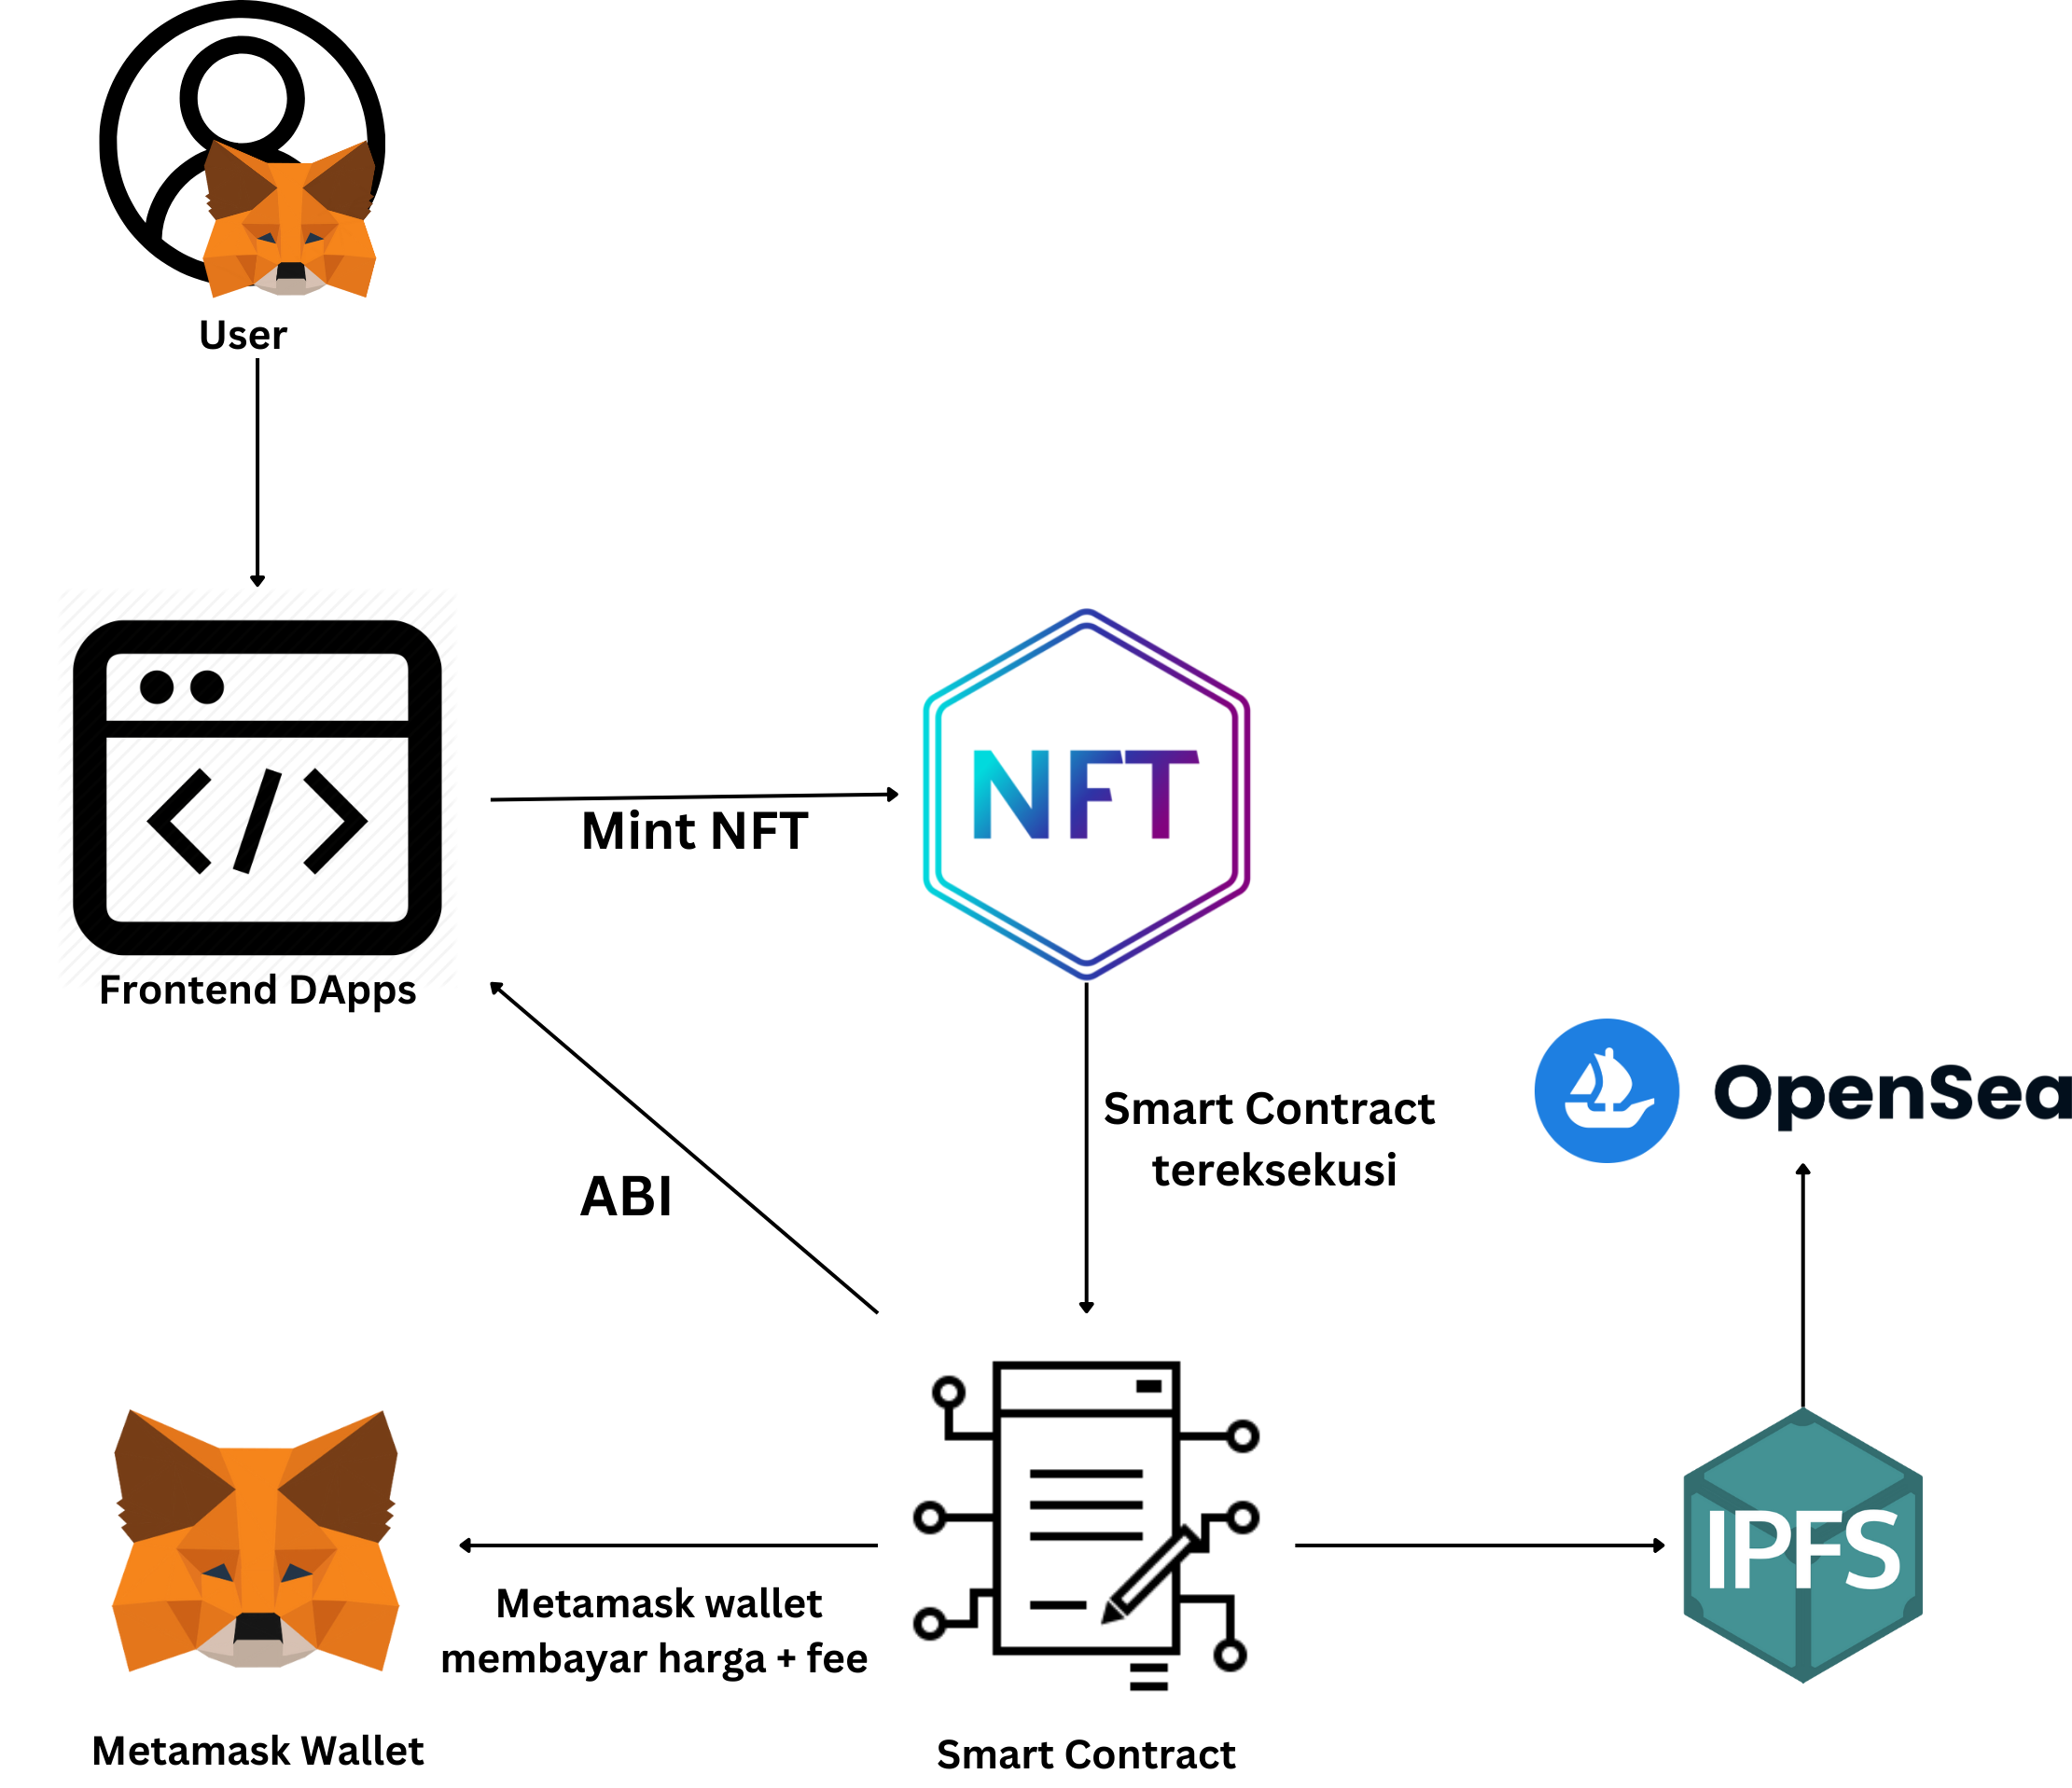
\includegraphics[scale=0.17]{gambar/desain_sistem_new.png}
  % Keterangan gambar yang diinputkan
  \caption{Arsitektur Sistem}
  % Label referensi dari gambar yang diinputkan
  \label{fig:flowtransaksi}
\end{figure}

Dalam pengembangan sistem \emph{smart contract} ini agar berjalan sesuai kehendak penulis untuk memenuhi tugas akhir ini, penulis membuat suatu arsitektur sistem. Pada arsitektur sistem ini, terdapat role \emph{user} yang dapat menjadi \emph{owner} dari suatu \emph{token} dan \emph{user} merupakan pihak yang memiliki akses terbatas terhadap suatu token dalam waktu yang telah ditentukan. Kemudian juga terdapat \emph{front end} untuk melakukan proses minting dari token NFT. Untuk dapat mengakses \emph{front end} baik owner ataupun user harus terhubung menggunakan wallet dari Metamask dalam berinteraksi.

Pada \emph{front end} akan terhubung dengan \emph{smart contract} ketika pengguna melakukan Minting dimana prosesnya pengguna mengunggah aset digital yang dimiliki dan diunggah ke IPFS melakukan aplikasi backend dan akan mengembalikan Content Identifier (CID). CID merupakan sebuah address file dalam IPFS yang digunakan untuk mengakses file tersebut. CID yang diperoleh kemudian akan diunggah ke jaringan \emph{blockchain} dan menjadi suatu token. Data-data mengenai NFT yang tersedia dapat langsung diperoleh \emph{frontend} melalui \emph{smart contract} pada \emph{blockchain}. 


\subsection{Flow Pembelian NFT}
\begin{figure} [H] \centering
  % Nama dari file gambar yang diinputkan
  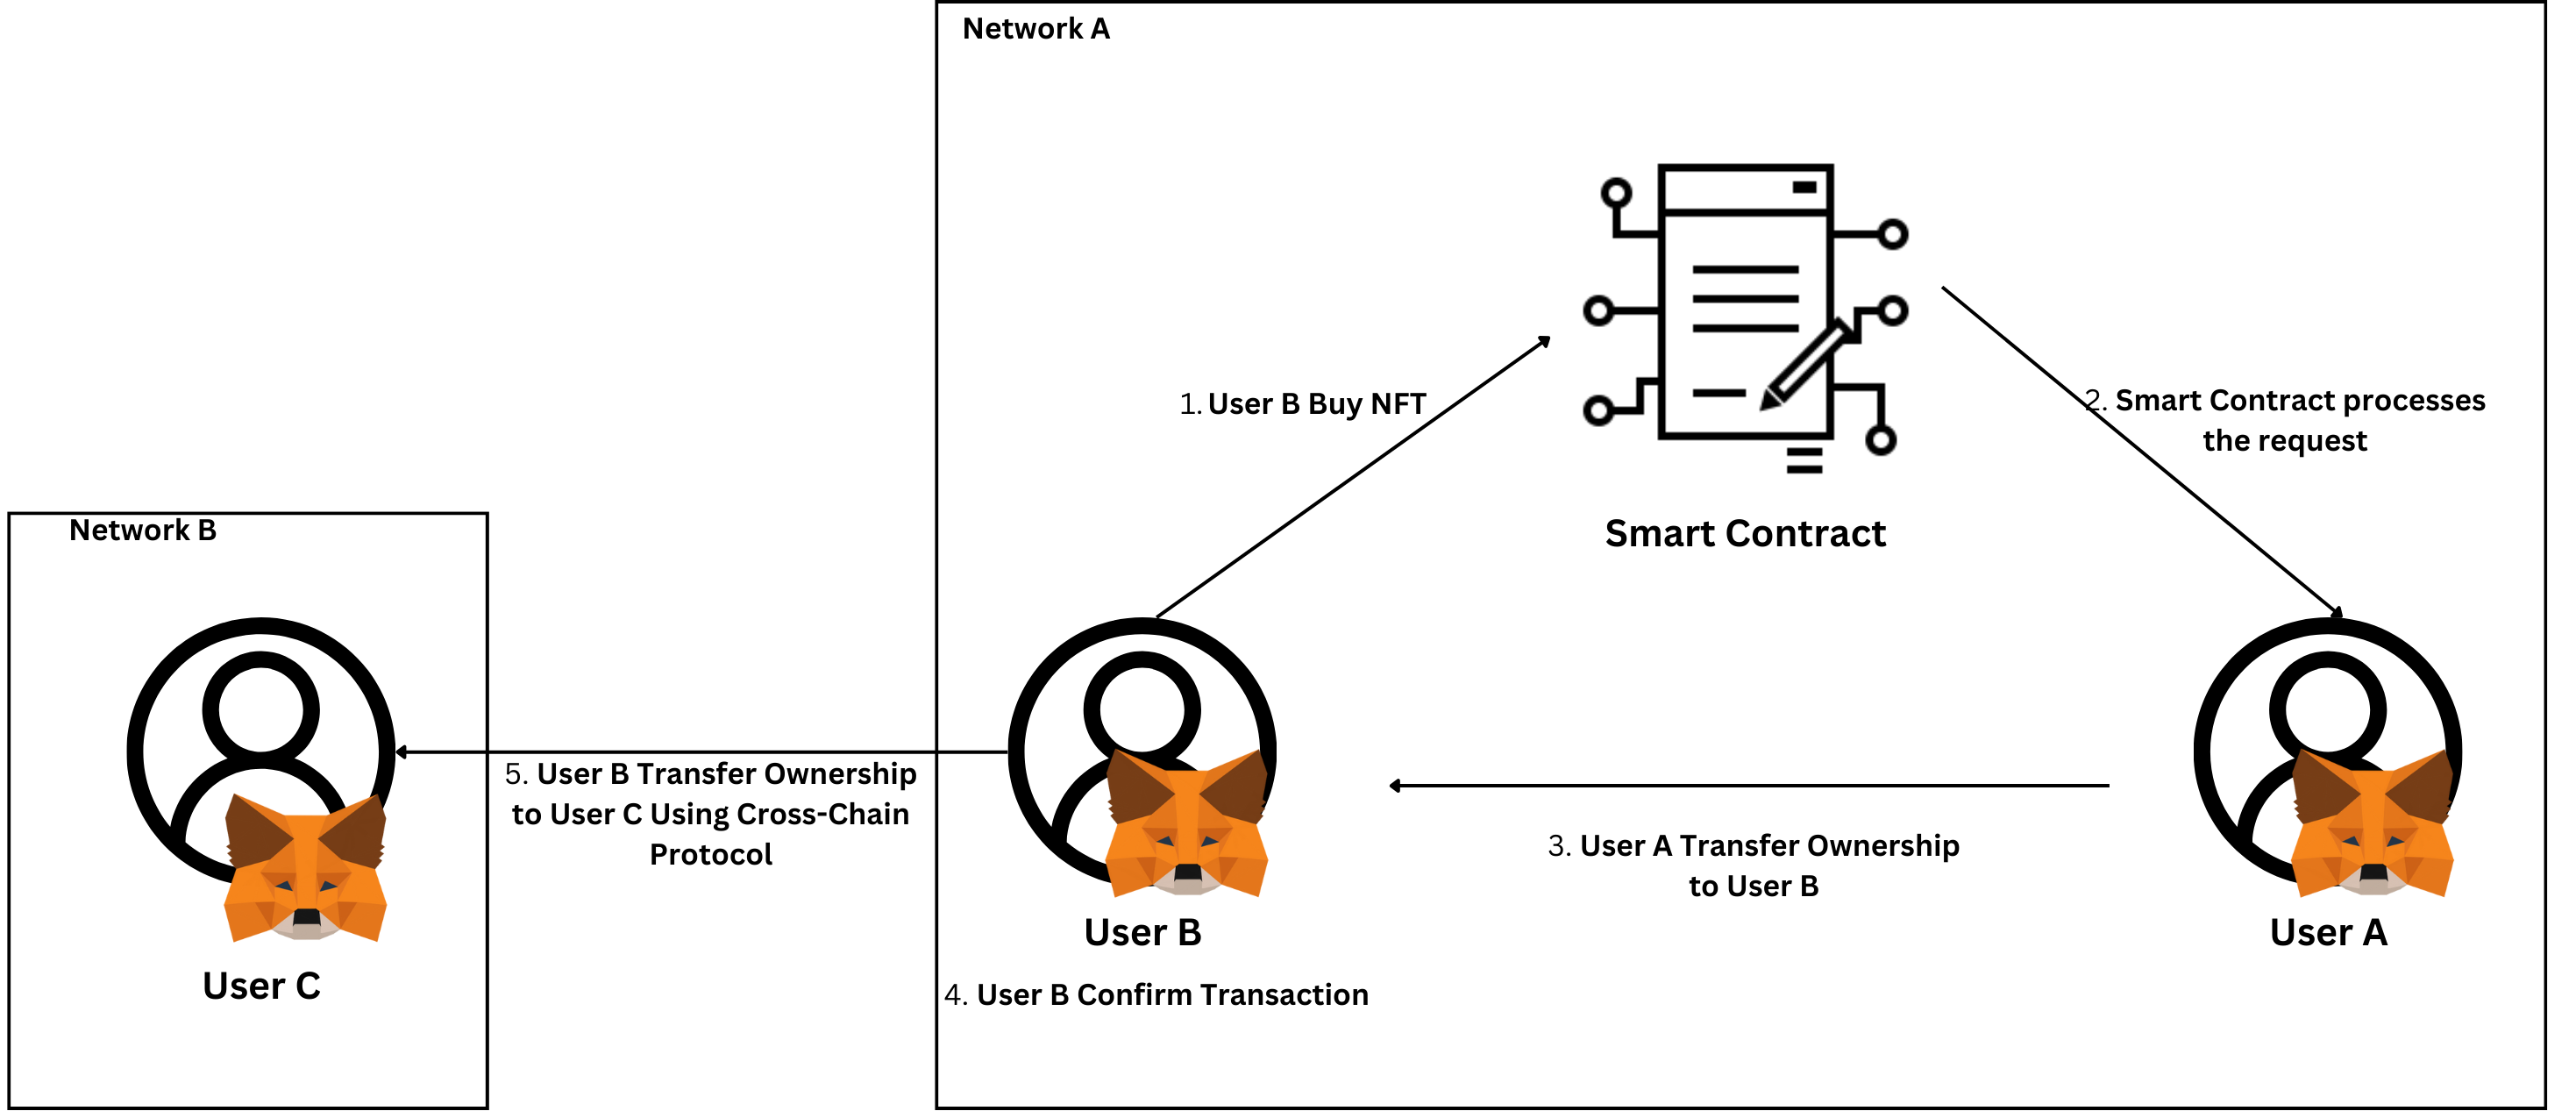
\includegraphics[scale=0.22]{gambar/flow_transaksi_new.png}
  % Keterangan gambar yang diinputkan
  \caption{Flow Pembelian NFT}
  % Label referensi dari gambar yang diinputkan
  \label{fig:flowtransaksi}
\end{figure}

Pada sistem ini terdapat juga fitur untuk melakukan pembelian NFT. Pembelian pada \emph{smart contract} yang akan dikembangkan menggunakan fungsi dari \emph{interface} token basis ERC-721. Interface ini memungkinkan token non-fungible diperjual belikan dalam satu kontrak. Kontrak ini akan tereksekusi ketika pengguna kedua (pembeli) melakukan pembelian token milik pengguna pertama (penjual). Kemudian pembeli melakukan minting NFT pada \emph{smart contract} dan juga penjual melakukan pemindahan kepemilikan dari NFT. Setelah proses itu selesai tereksekusi, pembeli mendapatkan NFT dan juga penjual mendapatkan mata uang kripto dari hasil penjualannya.

\subsection{Metadata}

\lstinputlisting[
  caption={Metadata pada NFT},
  label={lst:metadatanft}
]{program/A.json}

Dalam standar ERC-721, setiap NFT diwakili oleh metadata, yang merupakan kumpulan data mendetail mengenai konten Naturretnya dalam format JSON (JavaScript Object Notation). Metadata ini biasanya berisi informasi seperti nama, deskripsi, dan sebuah tautan ke gambar, yang semua dapat disesuaikan sesuai dengan kebutuhan aplikasi desentralisasi yang sedang dikembangkan. Struktur data ini disimpan dalam bentuk \emph{array} yang berisi objek-objek dalam format JSON, memungkinkan fleksibilitas tinggi dalam menyesuaikan data yang terkait dengan masing-masing NFT.

\subsection{Minting}
\begin{figure} [H] \centering
  % Nama dari file gambar yang diinputkan
  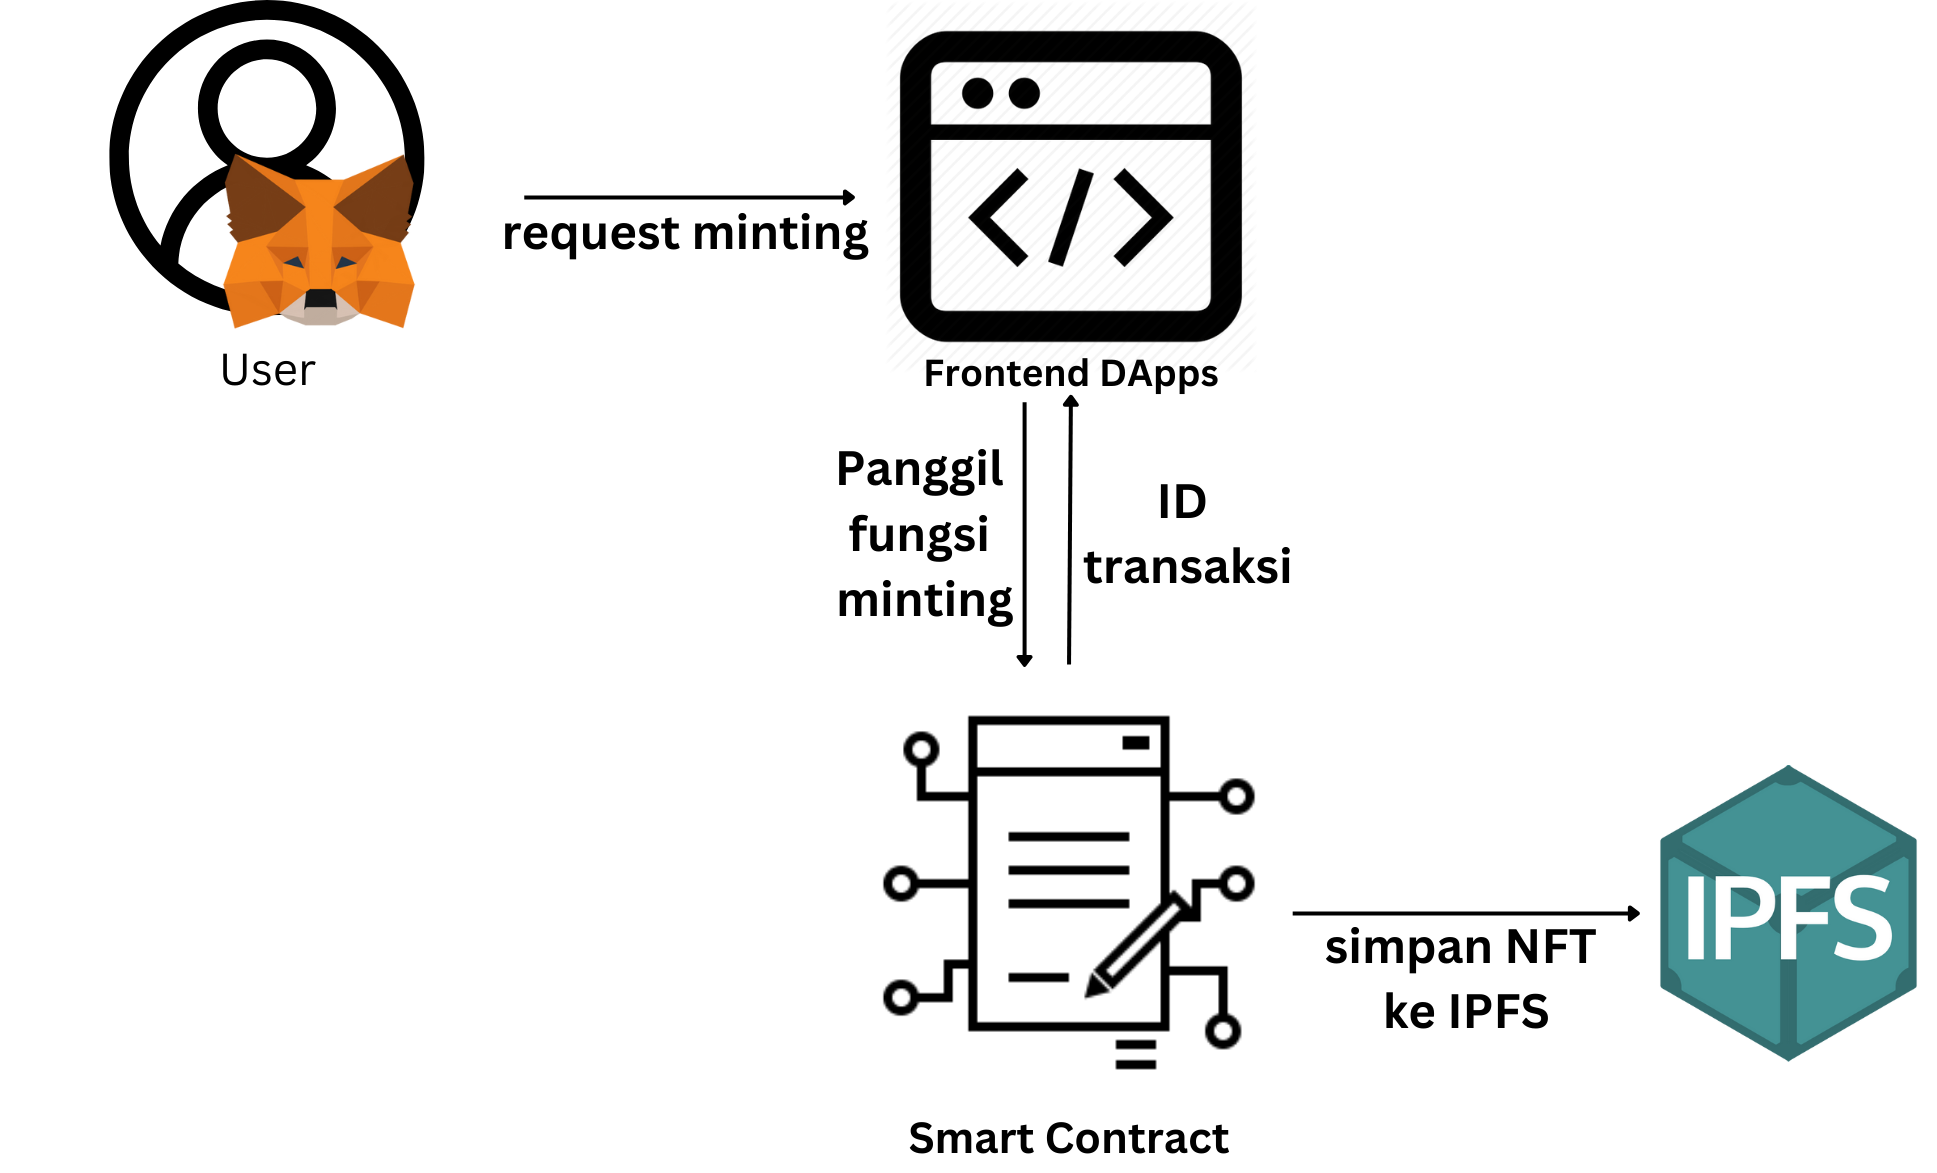
\includegraphics[scale=0.25]{gambar/proses_minting.png}
  % Keterangan gambar yang diinputkan
  \caption{Proses Minting}
  % Label referensi dari gambar yang diinputkan
  \label{fig:prosesminting}
\end{figure}


Proses \emph{minting} adalah langkah awal di mana sebuah NFT baru dibuat di dalam sebuah \emph{platform}. Selama proses ini, berbagai informasi penting tentang NFT tersebut harus ditentukan, termasuk nama, deskripsi, kategori, jumlah suplai yang tersedia, dan aset visual yang mewakili NFT, yang bisa berupa gambar 2D, model 3D, atau video. Harga awal, koleksi yang termasuk NFT, serta atribut lainnya juga perlu ditetapkan. Setelah proses minting selesai, data dari NFT yang baru dibuat ini akan disimpan dalam InterPlanetary File System (IPFS), yang memungkinkan penyimpanan dan akses data yang terdesentralisasi. Penyimpanan ini memastikan bahwa semua informasi terkait, seperti kepemilikan yang tercatat dalam atribut NFT, dapat diakses secara permanen dan aman.

\vspace{0.5 cm}

\section{Tools yang digunakan}
\label{sec:tools}
\subsection{Solidity}

Solidity adalah bahasa pemrograman tingkat tinggi yang secara khusus dirancang untuk mengembangkan \emph{smart contracts} pada platform \emph{blockchain} Ethereum. Bahasa ini menawarkan sintaks yang dioptimalkan untuk menangani operasi kontrak cerdas, termasuk dukungan untuk variabel, fungsi, dan struktur kontrol yang kompleks, yang semuanya vital dalam menciptakan aplikasi terdesentralisasi yang efisien dan aman. Selain itu, Solidity dilengkapi dengan berbagai fitur keamanan yang mencegah kerentanan umum seperti serangan \emph{reentrancy} dan \emph{overflows}. Keunggulan utama dari Solidity adalah kemampuannya untuk dijalankan di atas Ethereum Virtual Machine (EVM), lingkungan runtime yang menjadikannya kompatibel dengan berbagai jenis \emph{blockchain} yang mengadopsi standar EVM. Penggunaan Solidity membuka peluang bagi pengembang untuk menerapkan logika kontrak yang rumit yang bisa interaksi langsung dengan \emph{blockchain}, memberikan tingkat transparansi dan keandalan yang tinggi dalam transaksi digital.

\subsection{Metamask}

MetaMask adalah dompet digital yang dirancang khusus untuk memudahkan pengguna dalam mengelola aset kripto seperti Ether (ETH) dan berinteraksi dengan aplikasi terdesentralisasi (dApps) pada jaringan Ethereum. Fungsinya tidak hanya terbatas pada penyimpanan dan pengelolaan kripto, tetapi juga sebagai jembatan yang menghubungkan pengguna dengan ekosistem Ethereum. Sebagai ekstensi browser, MetaMask memungkinkan pengguna untuk melakukan transaksi kripto secara langsung dari browser web mereka tanpa perlu menggunakan perangkat lunak tambahan. MetaMask juga mendukung jaringan \emph{blockchain} lain yang kompatibel dengan Ethereum, memungkinkan pengguna untuk berpartisipasi dalam berbagai aktivitas \emph{blockchain} seperti game berbasis \emph{blockchain}, pasar seni digital, dan platform keuangan terdesentralisasi (DeFi). Dengan MetaMask, pengguna dapat dengan mudah beralih antara jaringan ini, menjelajahi dunia kripto dengan lebih aman dan nyaman.

\subsection{Hardhat}
Hardhat adalah kerangka kerja pengembangan \emph{smart contract} yang dirancang khusus untuk memudahkan proses pengembangan, pengujian, dan penyebaran \emph{smart contract}. Alat ini menyediakan serangkaian fitur yang memungkinkan pengembang \emph{blockchain} untuk bekerja lebih efisien. Dengan menggunakan Hardhat, pengembang dapat menjalankan lingkungan Ethereum lokal yang memudahkan proses pengujian dan debugging. Hardhat mendukung tugas otomatisasi yang kompleks dan mengintegrasikan stack perangkat lunak yang luas, termasuk plugin dan skrip yang dapat disesuaikan untuk meningkatkan fungsionalitas dan efisiensi. Framework ini juga memfasilitasi interaksi yang lebih mulus dengan jaringan Ethereum publik dan testnet, memungkinkan pengembang untuk memperoleh feedback yang cepat dan efektif tentang cara kerja \emph{smart contract} mereka di dalam kondisi jaringan yang sebenarnya.

\subsection{Ganache}

Ganache adalah alat simulasi \emph{blockchain} Ethereum yang digunakan secara luas dalam pengembangan dan pengujian \emph{smart contracts} dan aplikasi berbasis Ethereum. Ini memungkinkan pengembang untuk membuat jaringan \emph{blockchain} lokal yang dapat dijalankan di komputer mereka sendiri, mirip dengan jaringan Ethereum nyata, tetapi tanpa memerlukan sumber daya yang besar atau biaya transaksi yang sebenarnya.

\subsection{InterPlanetary File System}
InterPlanetary File System (IPFS) adalah protokol \emph{hypermedia} terdistribusi yang bertujuan untuk membuat web lebih cepat, aman, dan terbuka. IPFS telah menjadi populer di kalangan pengembang, terutama dalam pengembangan \emph{smart contract} untuk Non-Fungible Tokens (NFTs). Pada dasarnya, IPFS memungkinkan penyimpanan dan berbagi data dalam jaringan terdistribusi yang mirip dengan sistem peer-to-peer. Setiap file dan semua blok dalamnya diberi \emph{hash kriptografis} yang unik, yang bertindak sebagai alamat unik di jaringan.

Dalam konteks NFT, IPFS sangat berguna karena menyediakan solusi untuk tidak tergantung pada server tunggal atau lokasi penyimpanan yang bisa menjadi titik kegagalan. Misalnya, jika \emph{metadata} atau aset digital NFT seperti gambar, video, atau file audio disimpan hanya di server terpusat, ada risiko bahwa data tersebut bisa hilang atau dihapus. Menggunakan IPFS, file tersebut disimpan di beberapa node dalam jaringan, meningkatkan ketahanan dan ketersediaan data. Setiap kali file diminta, IPFS mengambil beberapa potongan dari banyak node, bukan mengambil seluruh file dari satu lokasi, mempercepat waktu pemuatan dan mengurangi beban pada jaringan.

\subsection{React.js}
React.js adalah sebuah pustaka JavaScript yang populer dan kuat untuk membangun antarmuka pengguna, atau lebih dikenal dengan istilah UI (\emph{User Interface}). Keunggulan React.js terletak pada kemampuannya untuk membangun aplikasi web yang dinamis dengan cara yang efisien dan mudah. React.js memungkinkan pengembang untuk membuat komponen UI yang besar dan kompleks, yang dapat dikelola dengan baik melalui penggunaan state dan props yang memberikan cara untuk \emph{data flow} dan \emph{re-rendering} yang efisien. 

Menggunakan React.js, pengembang dapat memanfaatkan library seperti Web3.js atau Ethers.js untuk berinteraksi langsung dengan \emph{blockchain Ethereum}, tempat \emph{smart contract} di-\emph{deploy}. Hal ini memungkinkan aplikasi untuk melakukan \emph{query} dan memperbarui \emph{blockchain} dengan transparan, menampilkan informasi seperti kepemilikan NFT, sejarah transaksi, dan \emph{metadata} NFT secara \emph{real-time}. 

\subsection{Web3.js}
Web3.js adalah sebuah pustaka JavaScript yang sangat penting untuk pengembangan aplikasi web yang berinteraksi dengan \emph{blockchain} Ethereum, khususnya dalam ekosistem Web 3.0. Library ini memungkinkan pengembang \emph{frontend} untuk berkomunikasi langsung dengan \emph{node} Ethereum, memanfaatkan fungsionalitas \emph{blockchain} seperti \emph{smart contracts}, transaksi, dan manajemen akun langsung dari browser pengguna.

Integrasi Web3.js dalam aplikasi React.js memungkinkan pengembang untuk memanfaatkan \emph{hook} dan komponen React untuk merespons perubahan \emph{state} pada \emph{blockchain} secara \emph{real-time}. Ini termasuk pembaruan saldo, perubahan status transaksi, dan pembaruan pada data \emph{smart contract}. Fungsi ini memperkuat pengalaman pengguna dengan memberikan tampilan yang konsisten dan \emph{up-to-date} dari status \emph{blockchain}, yang sangat penting dalam aplikasi yang menuntut keandalan dan transparansi tinggi.

\subsection{Ethers.js}
Ethers.js adalah sebuah \emph{library} JavaScript ringan yang dirancang untuk berinteraksi dengan Ethereum \emph{blockchain}. \emph{Library} ini sangat cocok untuk digunakan dalam pengembangan aplikasi \emph{frontend} dengan React.js karena menawarkan API yang sederhana dan modular, memudahkan pengembangan aplikasi desentralisasi (DApps) yang efisien. Ethers.js menyediakan fungsi-fungsi penting seperti penyambungan dengan \emph{wallet} pengguna, pembuatan dan pengiriman transaksi, serta interaksi dengan \emph{smart contract}.

Dalam pengembangan dengan React.js, Ethers.js membantu mengintegrasikan fungsi \emph{blockchain} ke dalam komponen React dengan cara yang bersih dan efektif. Misalnya, dengan menggunakan React \emph{hooks} seperti \emph{useState} dan \emph{useEffect}, pengembang dapat dengan mudah mengintegrasikan status dari \emph{Ethereum blockchain} ke dalam UI aplikasi, memperbarui UI secara \emph{real-time} ketika ada perubahan pada \emph{blockchain} seperti konfirmasi transaksi atau perubahan pada data \emph{contract}.

\subsection{Etherscan}
Etherscan adalah platform analitis berbasis web yang memungkinkan pengguna untuk melacak transaksi Ethereum, \emph{smart contract}, dan status \emph{blockchain} secara real-time. Platform ini memberikan wawasan mendetail tentang semua aktivitas yang terjadi di jaringan Ethereum, termasuk informasi tentang blok terbaru, transaksi yang sedang berlangsung, dan token yang beredar. Etherscan juga digunakan secara luas oleh pengembang untuk memeriksa dan memverifikasi kode sumber \emph{smart contract}, yang merupakan aspek penting dalam memastikan transparansi dan keamanan dalam ekosistem Ethereum. Dengan antarmuka yang mudah digunakan, Etherscan telah menjadi alat esensial bagi siapa saja yang terlibat dalam industri \emph{blockchain} Ethereum untuk memonitor, memverifikasi, dan menganalisis transaksi dan kontrak.

\subsection{Token ERC-721}
ERC-721 adalah standar untuk mewakili aset non-fungible (NFT) di \emph{blockchain} Ethereum. Standar ini memungkinkan representasi unik dari aset digital seperti karya seni, barang koleksi, dan item dalam game dalam bentuk token digital. Setiap token ERC-721 memiliki identifikasi unik dan dapat memiliki metadata yang terkait dengannya, yang membedakannya dari token lain di \emph{blockchain}. Fitur ini memfasilitasi pembuatan, perdagangan, dan penjualan aset digital dengan cara yang terdesentralisasi dan transparan. ERC-721 juga mendukung fungsi yang memungkinkan pemilik token untuk mentransfer, menyetujui, atau mengakses informasi tentang kepemilikan token, yang krusial untuk aplikasi di ekosistem Web3 dan ekonomi digital.

\section{Metode Yang Digunakan}

% Contoh input gambar dengan format *.jpg
\begin{figure} [H] \centering
  % Nama dari file gambar yang diinputkan
  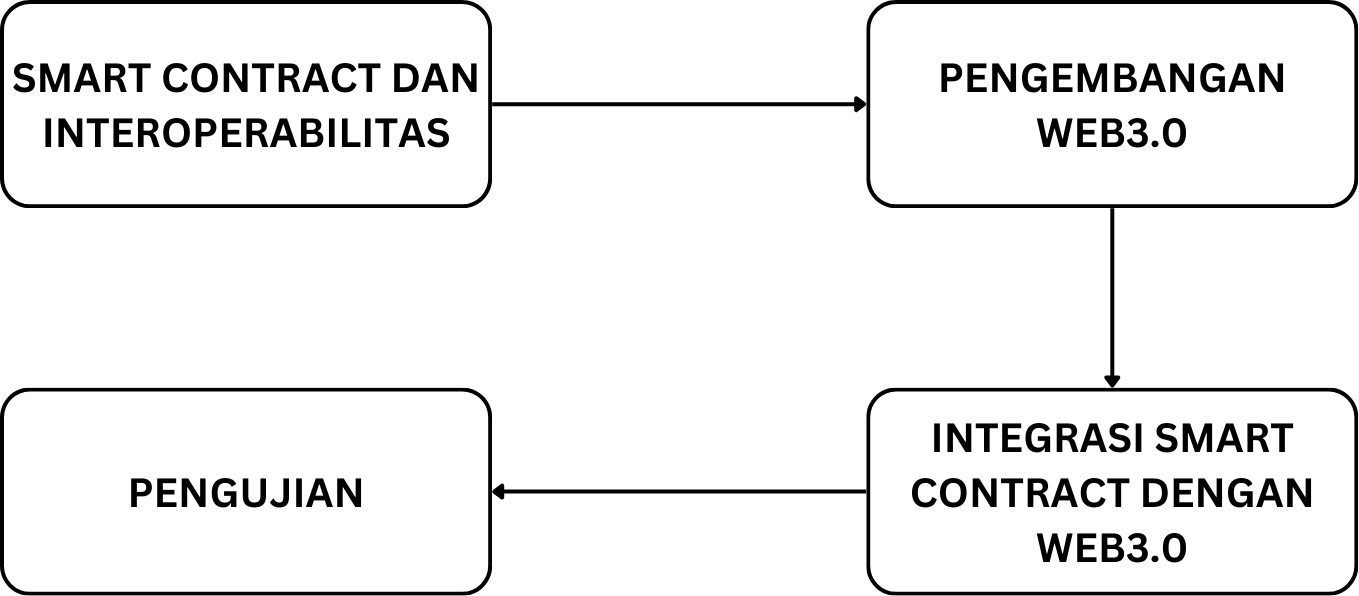
\includegraphics[scale=0.35]{gambar/metodologi_new_2.png}
  % Keterangan gambar yang diinputkan
  \caption{Metodologi Penelitian Yang Digunakan}
  % Label referensi dari gambar yang diinputkan
  \label{fig:flowtransaksi}
\end{figure}

\subsection{Smart Contract dan Interoperabilitas}
Pada tahapan ini, penulis mengembangkan sistem \emph{smart contract} yang digunakan untuk pembuatan token yang berinteroperabilitas menggunakan bahasa pemrograman Solidity. Sistem \emph{smart contract} ini digunakan sebagai jembatan untuk memperoses request dari yang dihasilkan dari interaksi pengguna pada \emph{frontend} ke jaringan \emph{blockchain}. Pada \emph{smart contract} yang telah di-\emph{compile} akan muncul ABI (\emph{Application Binary Interface}) yang dapat digunakan pada \emph{frontend} sebagai encoding dan decoding data yang memungkinkan \emph{frontend} aplikasi untuk mengirim instruksi yang tepat ke \emph{smart contract} dan memahami data yang dikembalikan olehnya. Dalam \emph{smart contract} yang dibuat oleh penulis terdapat beberapa fungsi yang dibuat sebagai inti pada token yang dikembangkan.

\subsubsection{Fungsi Mint}
Fungsi Mint dalam konteks \emph{smart contract } ERC-721 yang digunakan untuk \emph{minting} token NFT merupakan komponen krusial dalam mengelola penerbitan token baru. Ini diakses secara publik dan dapat menerima Ether, yang memungkinkan pembayaran langsung selama proses \emph{minting}.

\begin{lstlisting}[caption=Fungsi Mint]
FUNSI mint(_tokenURI: STRING) MENGEMBALIKAN BILANGAN BULAT:
    TAMBAHKAN tokenCount SEBANYAK 1
    JALANKAN _safeMint DENGAN PARAMETER (msg.sender, tokenCount)
    JALANKAN _setTokenURI DENGAN PARAMETER (tokenCount, _tokenURI)
    KEMBALIKAN tokenCount
AKHIR FUNGSI
\end{lstlisting}

\begin{itemize}
    \item \emph{Increment tokenCount}
    
    Pada awalnya, fungsi ini meningkatkan variabel \emph{tokenCount}. Variabel ini bertindak sebagai pengidentifikasi unik untuk setiap token baru; ini memastikan bahwa setiap token yang dicetak memiliki ID yang unik.

    \item \emph{Mint Token}
    
    Selanjutnya, fungsi memanggil metode \emph{\texttt{\_safeMint}}. Metode ini bertanggung jawab atas penciptaan token sebenarnya. Ini menetapkan kepemilikan token yang baru dicetak kepada pemanggil fungsi (\emph{msg.sender}), yang biasanya adalah pengguna yang berinteraksi dengan kontrak. Penggunaan \emph{\texttt{\_safeMint}} (dibandingkan \emph{\texttt{\_mint}}) memastikan pemeriksaan tambahan ada untuk mencegah token dikirim ke kontrak yang tidak siap untuk menanganinya, yang dapat mencegah kehilangan token secara tidak sengaja.

    \item \emph{Set Token URI}
    
    Setelah mencetak token, fungsi memperbarui metadata token dengan memanggil \emph{\texttt{\_tokenURI}}. Metode ini mengaitkan URI yang disediakan (\emph{\texttt{\_tokenURI}}) dengan ID token. URI biasanya mengarah ke file JSON yang di-\emph{host} secara eksternal yang berisi \emph{metadata} tentang token, seperti nama, deskripsi, dan URL gambar. Metadata ini memperkaya token dan dapat digunakan untuk memberikan informasi lebih rinci tentang aset digital.

    \item \emph{Return tokenCount}
    
    Terakhir, fungsi mengembalikan \emph{tokenCount}, yang merupakan pengidentifikasi unik dari token yang baru dicetak. ID ini dapat digunakan oleh aplikasi eksternal atau fungsi kontrak lain untuk merujuk token spesifik ini.
\end{itemize}

Secara keseluruhan, fungsi \emph{mint} ini sangat penting untuk menciptakan aset digital baru di \emph{blockchain}, memberikan pengguna kemampuan untuk menghasilkan NFT unik yang dapat mewakili segala sesuatu mulai dari seni digital hingga \emph{real estate virtual}, memastikan setiap aset dapat diidentifikasi secara jelas melalui ID token yang unik.
    
\subsubsection{Fungsi \emph{lockToken}}
\begin{lstlisting}[caption=Fungsi lockToken]
FUNGSI lockToken(tokenId: BILANGAN BULAT):
    PASTIKAN _exists(tokenId) = TRUE dengan pesan "Token does not exist."
    ATUR _locked[tokenId] = TRUE
    KIRIMKAN EVENT TokenLocked dengan (tokenId, msg.sender)
AKHIR FUNGSI
\end{lstlisting}

\begin{itemize}
    \item Pemeriksaan Keberadaan Token
    
    Fungsi ini memulai dengan memeriksa apakah token dengan ID yang diberikan benar-benar ada. Ini dilakukan melalui pemanggilan fungsi \emph{\texttt{\_exists}} yang memeriksa dalam basis data smart contract apakah token tersebut sudah dicetak dan masih ada. Jika token tidak ditemukan, fungsi akan memberikan error dan berhenti, dengan pesan "Token does not exist."

    \item Mengunci Token
    
    Jika token ditemukan, fungsi kemudian melanjutkan untuk mengunci token tersebut dengan mengatur nilai dari mapping \emph{\texttt{\_locked}} untuk tokenId yang bersangkutan menjadi true. Ini efektif membatasi fungsi smart contract yang dapat berinteraksi dengan token tersebut, khususnya mencegah transfer atau transaksi lain yang mungkin mengubah kepemilikan atau status token.

    \item Emit Event
    
    Setelah token berhasil dikunci, fungsi kemudian memicu event TokenLocked yang menandakan bahwa token telah dikunci. Event ini mencatat tokenId dan alamat yang memicu fungsi (biasanya pemilik atau pengontrol kontrak, sebagaimana ditandai oleh modifier onlyOwner). Event ini bisa digunakan untuk memberitahukan pengguna atau aplikasi lain yang berinteraksi dengan blockchain bahwa token tersebut sekarang berada dalam status terkunci dan tidak dapat dioperasikan atau dipindahkan hingga dibuka kunci.
\end{itemize}

Secara keseluruhan, fungsi \emph{lockToken} berperan penting dalam menjamin keamanan dan integritas transaksi yang melibatkan NFT, khususnya dalam skenario yang melibatkan operasi lintas rantai atau ketika sebuah token sedang menunggu konfirmasi transaksi yang kritis. Fungsi ini membantu memastikan bahwa tidak ada pihak yang tidak berwenang atau proses otomatis lainnya yang dapat mengganggu proses hukum atau komersial yang sedang berlangsung.

\subsubsection{Fungsi \emph{unlockToken}}
Fungsi unlockToken dalam \emph{smart contract} bertujuan untuk membuka kunci token yang sebelumnya telah dikunci. Fungsi ini sangat penting dalam manajemen aset dalam \emph{smart contract}, terutama dalam kasus penggunaan seperti transaksi lintas rantai atau ketika token harus dikunci untuk alasan keamanan atau administratif.

\begin{lstlisting}[caption=Fungsi unlockToken]
FUNGSI unlockToken(tokenId: BILANGAN BULAT)
    PASTIKAN _locked[tokenId] = TRUE dengan pesan "Token is not locked."
    ATUR _locked[tokenId] = FALSE
    KIRIMKAN EVENT TokenUnlocked dengan (tokenId, msg.sender)
AKHIR FUNGSI
\end{lstlisting}

\begin{itemize}
    \item Verifikasi Status Kunci
    
    Langkah pertama dalam fungsi ini adalah memastikan bahwa token yang ditentukan benar-benar dalam keadaan terkunci. Ini dilakukan dengan memeriksa mapping \emph{\texttt{\_locked}} untuk tokenId yang diberikan. Jika nilai dari mapping ini adalah false, yang berarti token tidak terkunci, maka fungsi akan menghasilkan error dan menghentikan eksekusi lebih lanjut dengan pesan "Token is not locked." Ini mencegah upaya untuk membuka kunci token yang tidak perlu atau yang mungkin telah secara tidak sengaja terbuka.

    \item Membuka Kunci Token
    
    Jika token memang terkunci, fungsi kemudian mengatur nilai dalam mapping \emph{\texttt{\_locked}} untuk tokenId tersebut menjadi false, secara efektif membuka kunci token tersebut. Ini mengizinkan token untuk berpartisipasi dalam transaksi dan interaksi lainnya sesuai dengan aturan smart contract lainnya.

    \item Emit Event
    
    Setelah token berhasil dibuka kunci, fungsi memicu event TokenUnlocked yang menandakan bahwa token tersebut telah dibuka kunci. Event ini mencatat tokenId dan alamat pengguna yang menjalankan fungsi (dijamin adalah pemilik atau pengontrol kontrak melalui penggunaan modifier onlyOwner). Event ini berguna untuk audit, pemantauan keamanan, dan sebagai bukti dalam aplikasi yang berinteraksi dengan smart contract bahwa token telah kembali ke status normal dan siap untuk dipindahkan atau digunakan.
\end{itemize}

Secara keseluruhan, fungsi unlockToken memainkan peran krusial dalam memastikan fleksibilitas dan keamanan dalam pengelolaan NFT dan aset digital lainnya. Fungsi ini memungkinkan pemilik atau pengontrol kontrak untuk secara efektif mengelola akses dan kontrol atas aset digital, memastikan bahwa aset tersebut hanya terkunci ketika benar-benar diperlukan dan bisa dibuka kembali ketika kondisi memungkinkan.

\subsubsection{Fungsi \emph{bridgeTransfer}}
Fungsi \emph{bridgeTransfer} dirancang untuk memungkinkan pemindahan token yang aman antara berbagai blockchain atau sub-jaringan, sebuah proses yang sering disebut sebagai "\emph{bridging}". Fungsi ini memastikan bahwa NFT (Non-Fungible Token) hanya dapat ditransfer setelah memenuhi kriteria keamanan tertentu.

\begin{lstlisting}[caption=Fungsi bridgeTransfer]
FUNGSI bridgeTransfer(_to: ALAMAT, _tokenId: BILANGAN BULAT)
    PASTIKAN _locked[_tokenId] = TRUE dengan pesan "Token must be locked before bridging"
    TRANSFER_TOKEN dari owner() ke _to dengan _tokenId
    KIRIMKAN EVENT TokenBridged dengan (_tokenId, owner(), _to)
AKHIR FUNGSI
\end{lstlisting}

\begin{itemize}
    \item Verifikasi Kondisi Kunci
    
    Langkah awal dalam fungsi ini adalah memastikan bahwa token yang ingin ditransfer sudah terkunci. Ini dilakukan dengan memeriksa nilai dari mapping \emph{\texttt{\_locked}} untuk tokenId yang diberikan. Jika token ini tidak terkunci, fungsi akan mengeluarkan kesalahan dan menghentikan proses lebih lanjut dengan pesan "\emph{Token must be locked before bridging}". Kondisi ini memastikan bahwa token hanya dipindahkan setelah melalui tahapan penguncian yang mencegah penggunaan atau transfer yang tidak sah sebelumnya.

    \item Eksekusi Transfer
    
    Setelah dipastikan bahwa token terkunci, fungsi selanjutnya melakukan transfer NFT dari pemilik saat ini ke alamat tujuan yang ditentukan (\emph{\texttt{\_to}}). Transfer ini dilakukan menggunakan fungsi \emph{\texttt{\_transfer}} yang merupakan bagian dari standar \emph{ERC-721}, memungkinkan perubahan kepemilikan NFT dalam \emph{blockchain}.

    \item Pencatatan Event
    
    Setelah transfer berhasil, fungsi mengirim event \emph{TokenBridged}. Event ini mencatat tokenId, alamat pemilik sebelum transfer (\emph{owner())}), dan alamat tujuan (\emph{\texttt{\_to}}). Event ini penting untuk audit dan pemantauan, memungkinkan aplikasi dan layanan yang terhubung untuk merespons atau mengakui transfer NFT lintas rantai.
\end{itemize}

Dengan cara ini, \emph{bridgeTransfer} menyediakan mekanisme yang efisien dan aman untuk mengintegrasikan fungsi interoperabilitas dalam \emph{smart contract} NFT, memungkinkan aset digital untuk berpindah antar ekosistem \emph{blockchain} sambil mempertahankan tingkat keamanan dan verifikasi yang ketat. Fungsi ini sangat penting dalam ekosistem \emph{blockchain} yang semakin terhubung, di mana NFT dan aset digital lainnya sering perlu beroperasi di berbagai platform dan jaringan.

\subsection{Pengembangan Frontend}
Pada tahap pengembangan frontend dalam proyek ini, kami memilih React.js sebagai kerangka kerja utama karena fleksibilitas dan efisiensinya dalam membangun antarmuka pengguna yang dinamis dan responsif. React.js memungkinkan pembuatan komponen yang dapat digunakan kembali, yang sangat meningkatkan efisiensi pengembangan dengan memungkinkan kami untuk membangun UI yang kompleks dari komponen yang lebih kecil dan termodularisasi.

Untuk mengintegrasikan aplikasi React dengan blockchain Ethereum, kami menggunakan dua pustaka utama: ethers.js dan web3.js. Kedua pustaka ini menyediakan fungsionalitas yang diperlukan untuk berinteraksi dengan Ethereum blockchain, tetapi dengan pendekatan yang sedikit berbeda. Ethers.js dikenal dengan API-nya yang minimalis dan mudah digunakan, yang sangat cocok untuk proyek-proyek dengan kebutuhan yang lebih sederhana dan lebih fokus pada pembacaan serta penulisan data ke blockchain. Pustaka ini menyediakan fungsi yang kuat untuk berinteraksi dengan smart contracts, seperti mengirim transaksi, membaca status kontrak, dan menangani notifikasi event.

Di sisi lain, web3.js adalah pustaka yang lebih luas yang sering digunakan untuk proyek yang memerlukan integrasi yang lebih kompleks dengan Ethereum. Web3.js menyediakan modul yang lebih komprehensif dan mendukung interaksi yang lebih beragam dengan blockchain, termasuk pengelolaan akun, komputasi gas, dan langganan event yang lebih canggih. Kedua pustaka ini, ketika digunakan bersama-sama atau secara terpisah, memberikan fleksibilitas yang sangat dibutuhkan dalam pengembangan frontend untuk aplikasi berbasis blockchain.

\subsection{Integrasi Smart Contract dengan Frontend}
Pada tahap ini memungkinkan aplikasi yang dibangun dengan React.js untuk berinteraksi secara langsung dengan smart contract yang telah dideploy di jaringan Ethereum. Untuk mencapai integrasi ini, kami menggunakan pustaka ethers.js, yang menyediakan antarmuka yang bersih dan mudah digunakan untuk berkomunikasi dengan Ethereum.

Setelah smart contract dikembangkan dan dideploy, ABI (Application Binary Interface) dari contract tersebut digunakan untuk membangun sebuah instance contract dalam aplikasi React. ABI memungkinkan frontend untuk mengetahui fungsi-fungsi apa saja yang tersedia dalam smart contract, termasuk variabel dan tipe data yang digunakan. Dengan informasi ini, ethers.js dapat memanggil fungsi-fungsi tersebut seperti fungsi safeMint atau transferOwnership, sesuai dengan logika yang didefinisikan dalam contract.

Dalam aplikasi, kami mengonfigurasi ethers.js untuk terhubung dengan provider Ethereum, yang bisa berupa MetaMask atau node Ethereum lainnya. Ini memungkinkan aplikasi untuk mengirim transaksi dan memantau event yang diterbitkan oleh smart contract. Setiap kali pengguna berinteraksi dengan UI, seperti mengklik tombol untuk memint NFT atau mentransfer kepemilikan, permintaan tersebut diterjemahkan oleh ethers.js menjadi transaksi blockchain yang sesuai.

Selain itu, untuk meningkatkan keamanan dan keandalan aplikasi, kami juga mengimplementasikan penanganan error yang robust untuk mengatasi masalah yang mungkin terjadi selama interaksi dengan blockchain, seperti kegagalan transaksi atau masalah konektivitas. Dengan demikian, pengguna dapat menerima feedback yang tepat waktu dan akurat jika ada masalah yang terjadi selama proses transaksi.

\subsection{Pengujian}
Pada tahap ini terdapat beberapa langkah pengujian \emph{smart contract} yaitu pengujian unit dan juga pengujian integrasi.

\begin{itemize}
    \item Pengujian Unit
    Pada pengujian ini adalah fokus dalam memvalidasi setiap komponen secara individual. Dalam konteks frontend React.js, ini berarti menguji komponen-komponen secara terpisah untuk memastikan bahwa mereka berperilaku sesuai dengan ekspektasi. Pengujian unit juga dilakukan pada fungsi-fungsi smart contract untuk memverifikasi logika bisnisnya, seperti fungsi minting atau transfer token. Pengujian ini biasanya dilakukan dengan bantuan framework React untuk frontend dan  Hardhat untuk smart contracts.

    \item Pengujian Integrasi
    Setelah pengujian unit, langkah berikutnya adalah pengujian integrasi, yang memastikan bahwa semua komponen dalam aplikasi bekerja dengan baik saat digabungkan. Dalam konteks integrasi smart contract, ini melibatkan menguji interaksi antara frontend React.js dan smart contract melalui ethers.js atau web3.js. Pengujian integrasi membantu mendeteksi masalah pada alur data antara frontend dan blockchain, termasuk validasi transaksi dan pembaruan state yang benar.
\end{itemize}

\cleardoublepage

% Bab 4 pengujian dan analisis
\chapter{HASIL DAN PEMBAHASAN}
Pada subbab pertama pada bab ini akan dipaparkan hasil akhir dari pengerjaan tugas akhir Interoperabilitas NFT Berbasis \emph{Blockchain} Menggunakan \emph{Smart Contract} pada WEB3.0. Pada subbab selanjutnya akan dipaparkan mengenai hasil pengujian dari hasil tugas akhir untuk memastikan bahwa sistem yang dikembangkan berjalan dengan sesuai.

\section{Hasil}
Hasil keseluruhan dari sistem yang dikembangkan adalah \emph{interface} berupa web, \emph{Non-Fungible Token} (NFT) dan juga \emph{smart contract} yang berinteroperabilitas. Berikut dipaparkan masing-masing hasil dari sistem yang dikembangkan.

\subsection{Web Interface}
Tampilan awal web \emph{interface}, menampilkan daftar koleksi NFT yang dapat di-\emph{minting}. Nantinya NFT tersebut dapat dimiliki oleh \emph{address} yang melakukan pertama kali \emph{minting} dan juga kepemilikan dari NFT tersebut dapat diberikan ke \emph{address} lain.
\begin{figure} [H] \centering
  % Nama dari file gambar yang diinputkan
  \frame{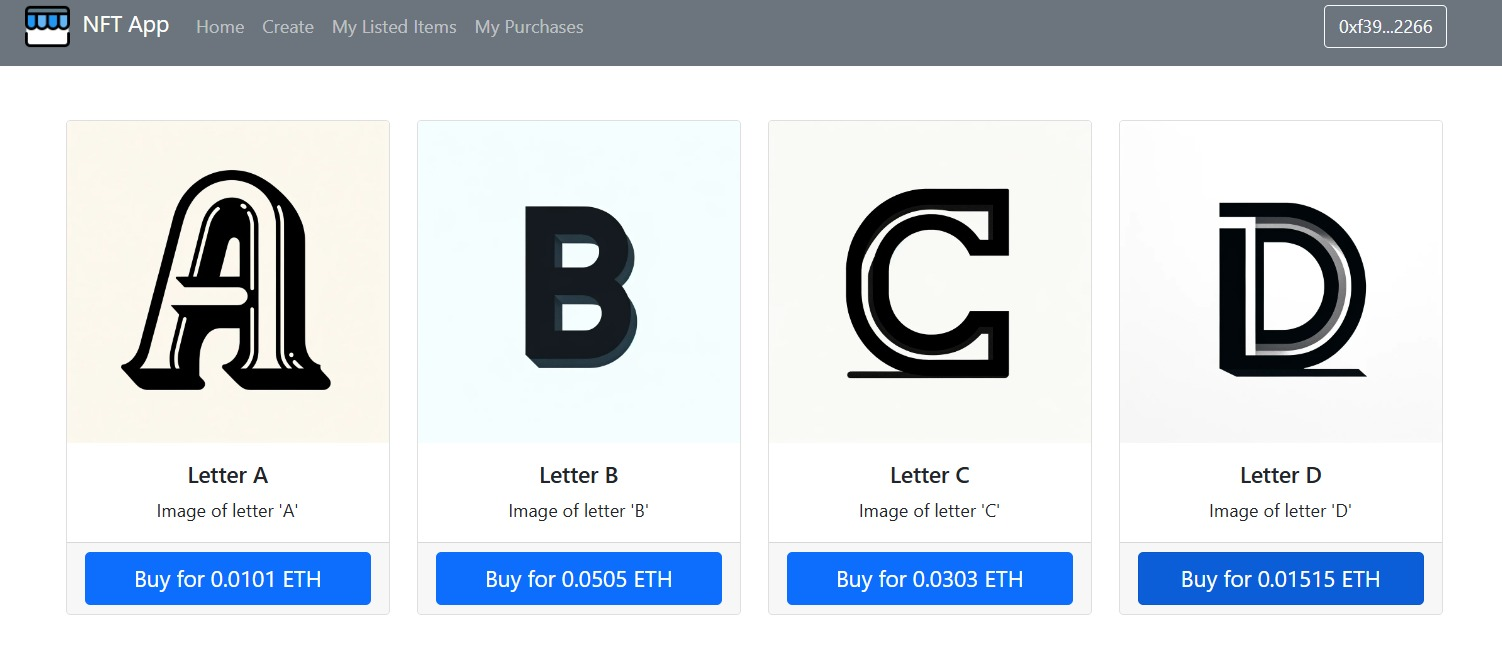
\includegraphics[scale=0.30]{gambar/tampilan_aplikasi.jpeg}}
  % Keterangan gambar yang diinputkan
  \caption{Tampilan interface}
  % Label referensi dari gambar yang diinputkan
  \label{fig:interface}
\end{figure}

Pada halaman dashboard awal, pengguna diharuskan untuk menekan tombol Connect Wallet, yang akan memicu proses koneksi dengan Metamask Wallet. Setelah berhasil terhubung, pengguna akan mendapatkan address yang bersifat unik. Alamat ini tidak hanya penting untuk keperluan identifikasi pengguna di dalam jaringan, tetapi juga berfungsi sebagai kunci akses untuk melakukan minting token NFT. Dengan demikian, address tersebut menjadi sangat krusial karena merupakan representasi digital dari identitas pengguna dalam ekosistem blockchain, memungkinkan mereka untuk bertransaksi, mengakses, dan mengelola aset digital mereka dengan aman. Proses ini memastikan bahwa setiap interaksi yang dilakukan melalui smart contract untuk NFT tercatat secara transparan dan dapat diverifikasi, memberikan keamanan dan kepercayaan dalam setiap transaksi.

  \begin{figure} [H] \centering
  % Nama dari file gambar yang diinputkan
  \frame{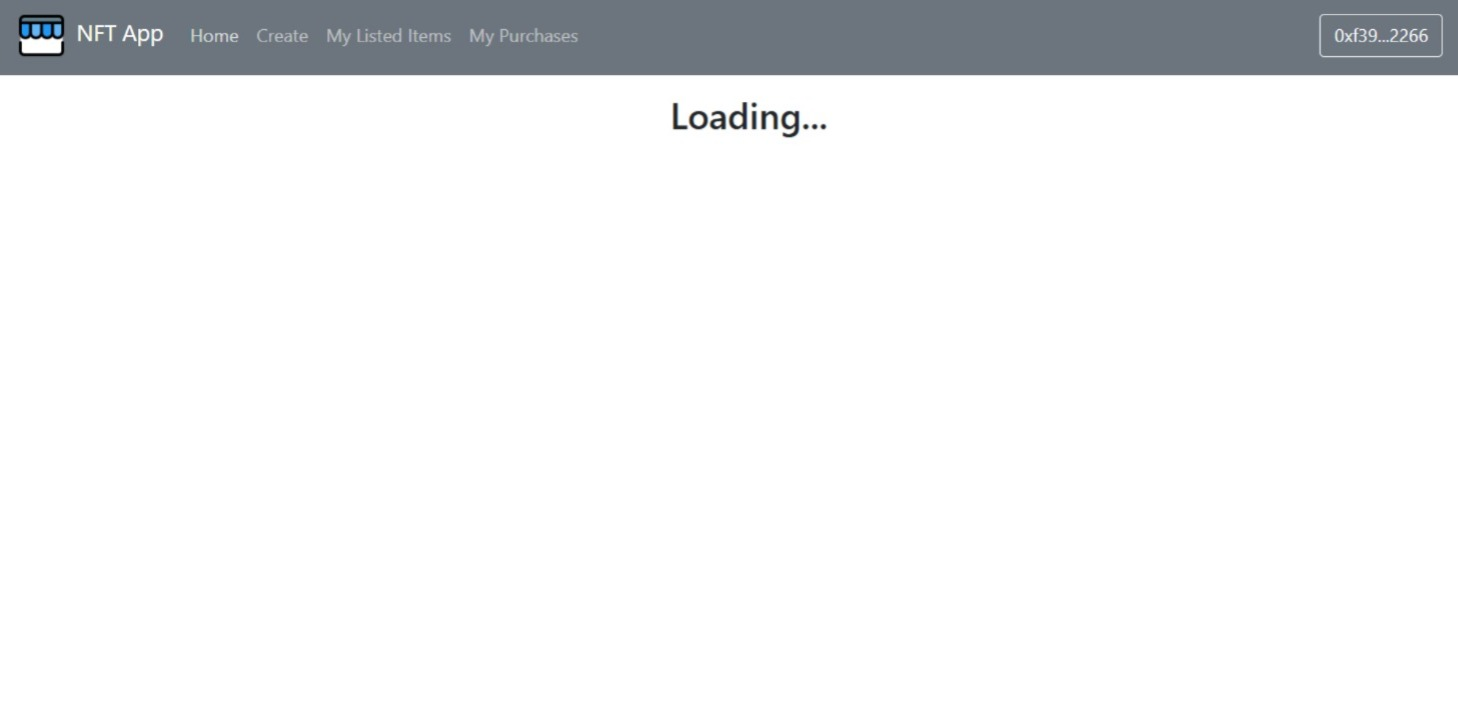
\includegraphics[scale=0.27]{gambar/home_page.jpg}}
  % Keterangan gambar yang diinputkan
  \caption{Tampilan awal dari web}
  % Label referensi dari gambar yang diinputkan
  \label{fig:homepage}
  \end{figure}

  Pada gambar \ref{fig:homepage} adalah tampilan dari \emph{homepage} awal ketika pengguna menekan tombol \emph{home} pada \emph{navigation bar} atas. Pada web ini terdapat beberapa halaman yang dapat diakses dengan menekan tombol pada \emph{navigation bar}, seperti \emph{Home}, \emph{Create}, \emph{My Listed Items}, dan \emph{My Purchase}. Tampilan-tampilan ini dapat diakses ketika pengguna telah melakukan koneksi web dengan Metamask Wallet, hal ini dapat dilihat pada \emph{navigation bar} atas kanan terdapat \emph{address} dari akun Metamask Wallet. Pada tampilan awal ini, pengguna dapat melihat NFT yang telah diunggah untuk dapat dilakukan pembelian atau \emph{minting}. Tetapi karena belum terdapat NFT yang diunggah maka hanya akan menampilkan tulisan "\emph{Loading...}".
   
  \begin{figure} [H] \centering
    % Nama dari file gambar yang diinputkan
    \frame{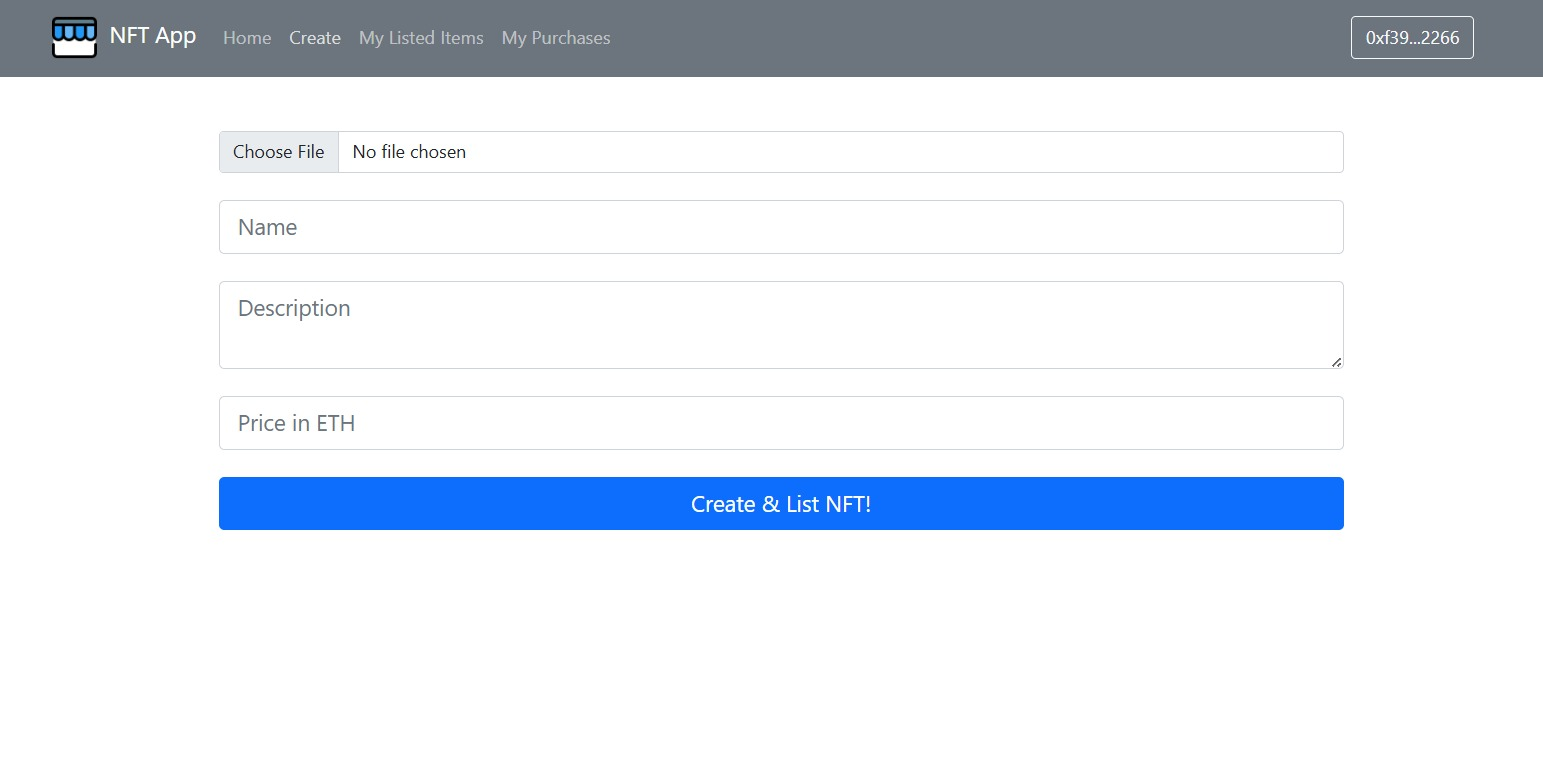
\includegraphics[scale=0.27]{gambar/create_page.jpeg}}
    % Keterangan gambar yang diinputkan
    \caption{Tampilan halaman \emph{create}}
    % Label referensi dari gambar yang diinputkan
    \label{fig:createpage}
    \end{figure}

  Pada gambar \ref{fig:createpage} adalah tampilan dari \emph{create page}. Pada halaman ini pengguna dapat mengunggah sebuah NFT berupa gambar ke web yang kemudian jika diunggah akan muncul pada halaman \emph{home} dan juga akan muncul pada halaman \emph{my listed items}.

  \begin{figure} [H] \centering
    % Nama dari file gambar yang diinputkan
    \frame{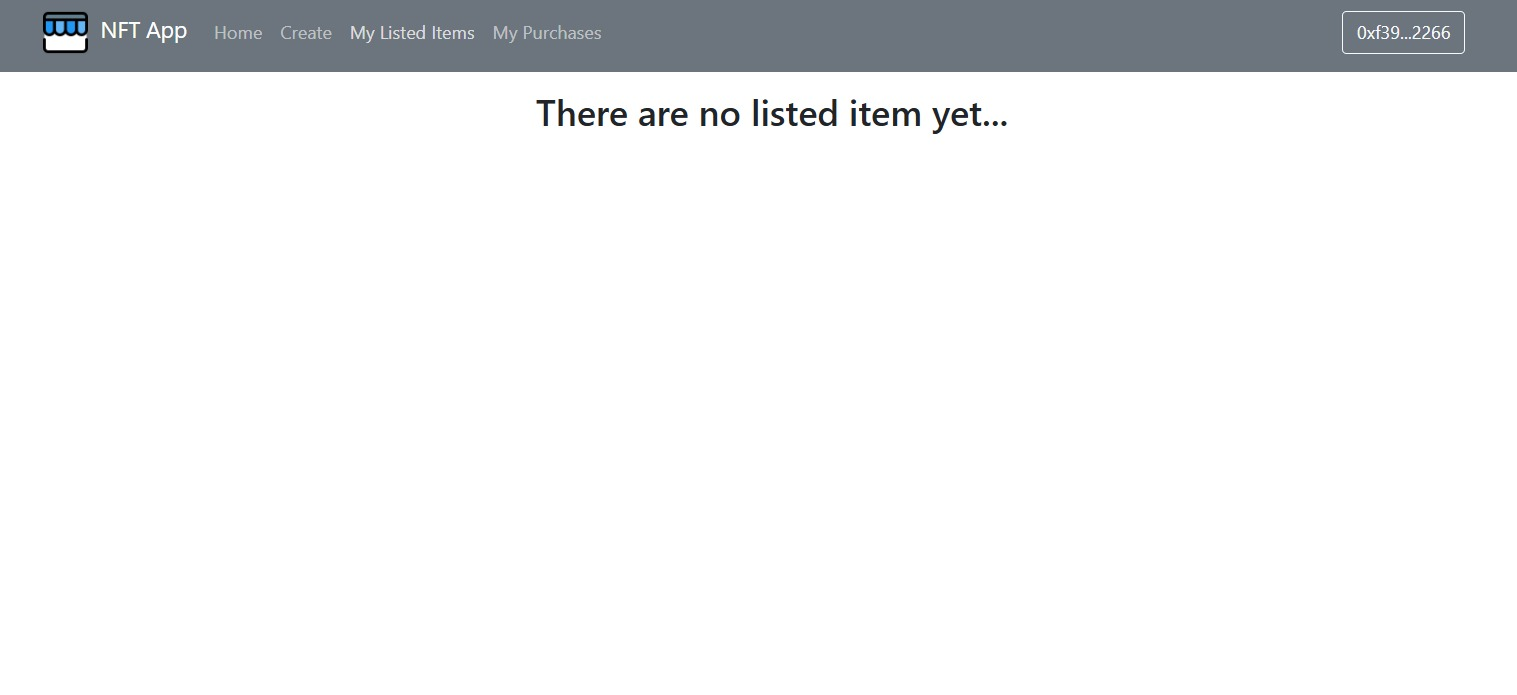
\includegraphics[scale=0.27]{gambar/listing_page.jpg}}
    % Keterangan gambar yang diinputkan
    \caption{Tampilan halaman \emph{my listed items}}
    % Label referensi dari gambar yang diinputkan
    \label{fig:listingpage}
    \end{figure}
  
  Pada gambar \ref{fig:listingpage} adalah tampilan dari \emph{my listed items page}. Pada halaman ini pengguna dapat melihat NFT kepemilikannya yang telah diunggah pada ketika dia melakukan \emph{create}. Tetapi dikarenakan belum melakukan pengunggahan NFT, maka halaman ini hanya akan memunculkan tulisan "\emph{There are no listed item yet}".

  \begin{figure} [H] \centering
    % Nama dari file gambar yang diinputkan
    \frame{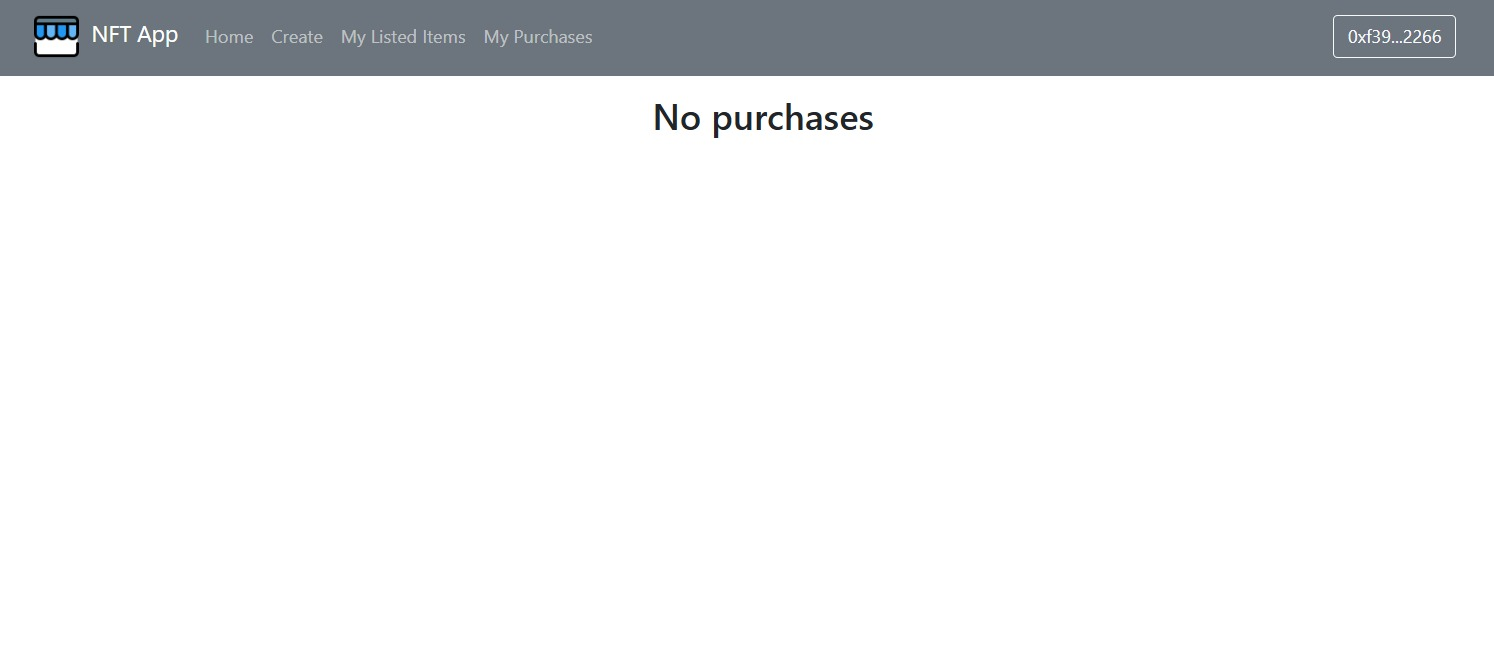
\includegraphics[scale=0.27]{gambar/purchase_page.jpg}}
    % Keterangan gambar yang diinputkan
    \caption{Tampilan halaman \emph{my purchases}}
    % Label referensi dari gambar yang diinputkan
    \label{fig:purchasepage}
    \end{figure}
  
  Pada gambar \ref{fig:purchasepage}, terlihat tampilan dari \emph{my purchase page} yang dirancang khusus untuk memungkinkan pengguna melihat semua NFT yang telah mereka peroleh melalui pembelian di halaman utama platform. Setelah melakukan pembelian, NFT tersebut akan terdaftar di halaman ini, memberikan tampilan visual serta detail dari setiap NFT yang dimiliki. Lebih lanjut, halaman ini juga menyediakan fungsi \emph{transfer ownership}, yang memungkinkan pemilik untuk mengalihkan kepemilikan NFT kepada pengguna lain dengan \emph{address} yang berbeda. Fungsi ini sangat penting untuk mendukung fleksibilitas dan likuiditas dalam perdagangan NFT di pasar. Namun, jika pengguna belum melakukan pembelian apapun, halaman ini akan menampilkan pesan "\emph{No purchases}", yang menandakan bahwa tidak ada NFT yang dapat ditampilkan atau ditransfer.z

\subsection{\emph{Smart Contract}}
Dalam pengembangan aplikasi berbasis \emph{blockchain}, pengintegrasian \emph{smart contract} dengan antarmuka pengguna seperti React.js menjadi krusial. \emph{Smart contract} yang dibangun menggunakan Solidity dapat di-\emph{deploy} di \emph{testnet} Ethereum, seperti Sepolia Testnet, yang menyediakan lingkungan yang hampir mirip dengan mainnet Ethereum namun tanpa memerlukan biaya transaksi yang besar. 

ABI atau \emph{Application Binary Interface}, adalah cara yang memungkinkan fungsi dalam \emph{smart contract} Ethereum untuk berkomunikasi dengan aplikasi eksternal, termasuk antarmuka pengguna yang dibangun dengan kerangka kerja seperti React.js. ABI berperan sebagai lapisan translasi yang menguraikan cara memanggil fungsi dalam smart contract, jenis parameter yang diterima, jenis keluaran yang diharapkan, serta sifat state dari fungsi tersebut. ABI biasanya dihasilkan secara otomatis oleh \emph{compiler} Solidity sebagai bagian dari proses kompilasi \emph{smart contract} dan disimpan dalam format JSON. Setiap kali aplikasi \emph{frontend} mengirimkan transaksi atau \emph{query} ke \emph{blockchain}, ia menggunakan ABI untuk mengkodekan data panggilan ke dalam format yang dapat dipahami oleh \emph{Ethereum Virtual Machine} (EVM). Kemudian, saat data dikembalikan dari \emph{smart contract}, ABI digunakan untuk mendekode balasan sehingga aplikasi React.js dapat memahami dan memprosesnya.

Proses \emph{deploy} dilakukan \emph{smart contract} akan di-\emph{deploy} ke beberapa jaringan \emph{blockchain} namun dikarenakan dalam pengujian ini yang digunakan adalah sepolia \emph{testnet} maka yang digunakan hanyalah dari jaringan sepolia \emph{testnet}. Ketika melakukan proses \emph{deployment} akan dikenakan \emph{gas} atau fee yang dapat dibayar menggunakan \emph{ethereum} yang terdapat pada \emph{wallet} Metamask. Yang kemudian detail dari transaksi tersebut dapat dilihat pada Etherscan.

\begin{figure} [H] \centering
  % Nama dari file gambar yang diinputkan
  \frame{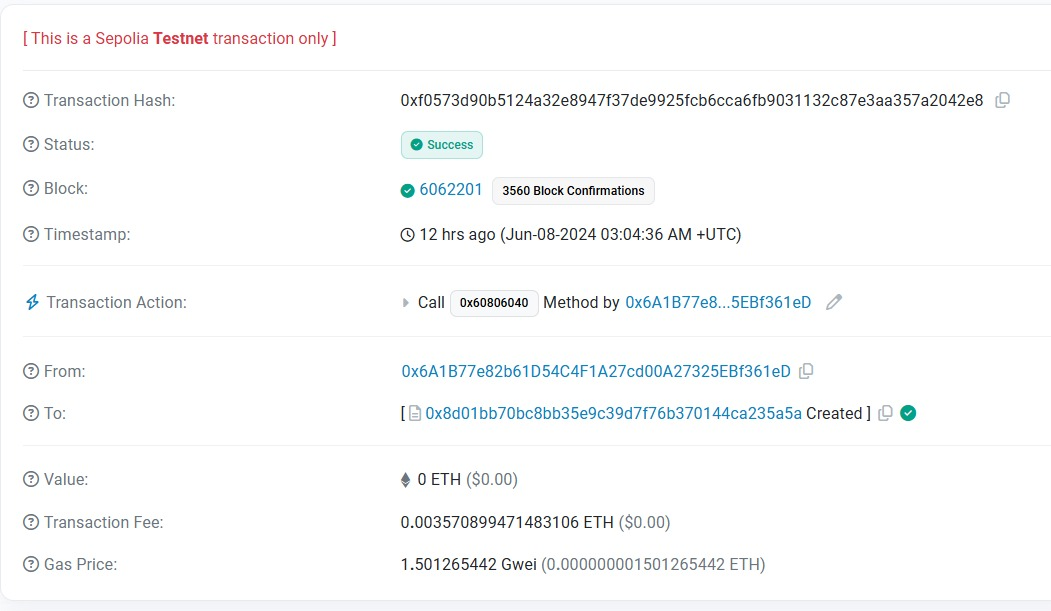
\includegraphics[scale=0.45]{gambar/etherscan.jpeg}}
  % Keterangan gambar yang diinputkan
  \caption{Detail transaksi pada etherscan}
  % Label referensi dari gambar yang diinputkan
  \label{fig:transaction}
\end{figure}

\subsection{\emph{Non-Fungible Token} (NFT)}
\emph{Non-Fungible Token} (NFT) sendiri juga memiliki beberapa tahapan agar dapat dapat disimpan dalam \emph{The Interplanetary File System} (IPFS) dan kemudian dapat di-\emph{publish} pada OpenSea \emph{test net}. Pada pengerjaan tugas akhir ini, Pinata digunakan sebagai \emph{platform} untuk mengunggah foto NFT dan juga data \emph{JavaScript Object Notation} (JSON) agar bisa di-\emph{minting} sebagai \emph{Uniform Resource Identifier} (URI) pada \emph{smart contract}. Hal ini dibutuhkan agar NFT yang di-\emph{minting} memiliki gambar yang dapat dilihat pada OpenSea.

\begin{figure} [H] \centering
  % Nama dari file gambar yang diinputkan
  \frame{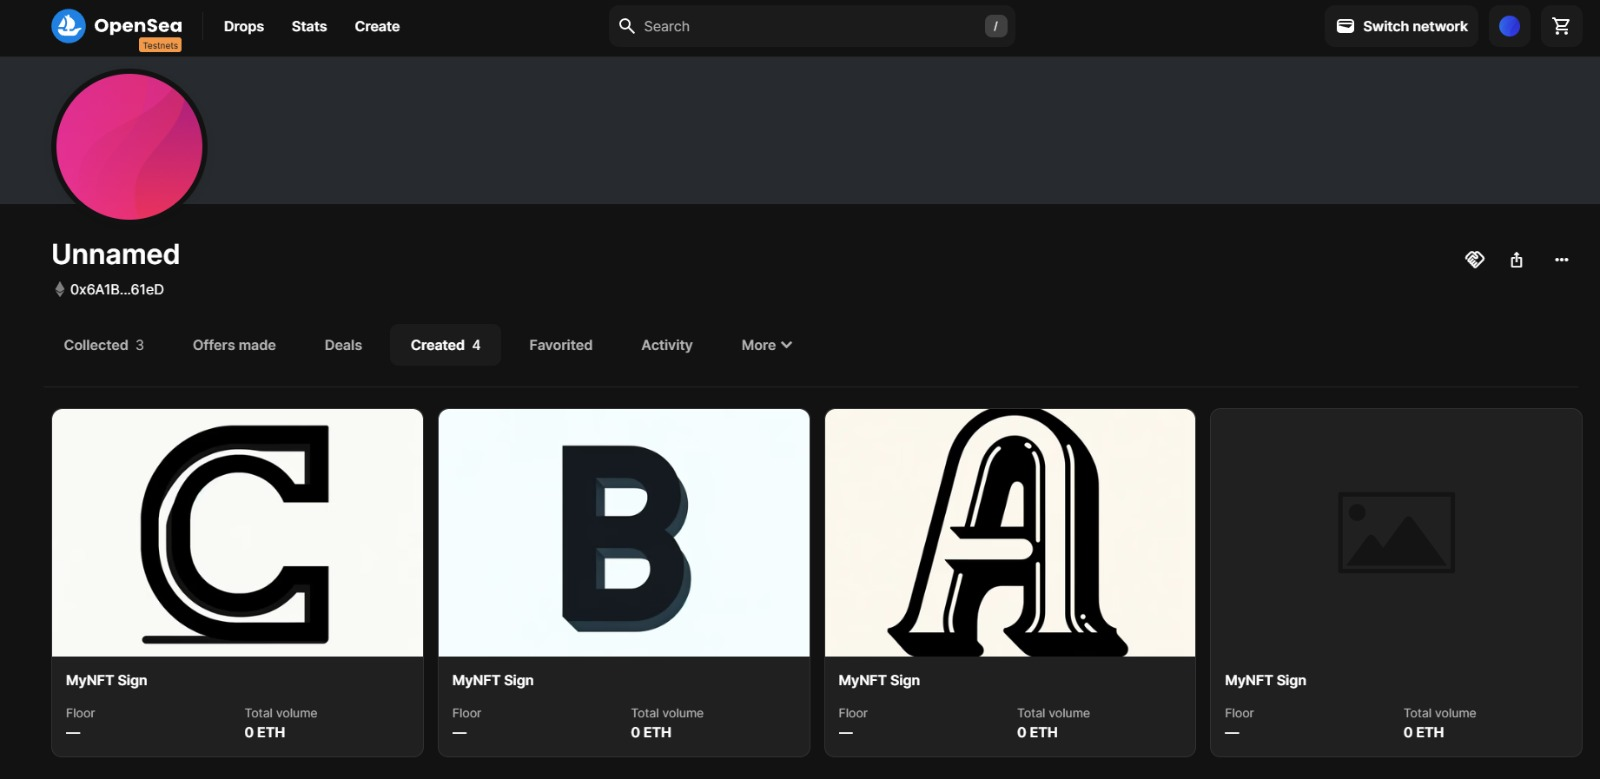
\includegraphics[scale=0.28]{gambar/opensea.jpeg}}
  % Keterangan gambar yang diinputkan
  \caption{NFT terunggah pada Opensea}
  % Label referensi dari gambar yang diinputkan
  \label{fig:opensea}
\end{figure}

\section{Pengujian}
Untuk memastikan bahwa sistem interoperabilitas \emph{Smart Contract} berjalan sesuai dengan yang direncakan maka perlu dilakukan pengujian lebih lanjut. Pengujian yang dilakukan secara garis besar dibagi menjadi dua yaitu Pengujian fitur-fitur utama dari \emph{Smart Contract} yang meliputi \emph{minting}, \emph{lock}, dan \emph{bridge transfer} kepemilikan NFT dan yang kedua adalah pengujian integrasi ke \emph{interface} yang telah dibuat. Berikut merupakan paparan dari pengujian.

\subsection{Pengujian Fitur \emph{Smart Contract}}
Ekspektasi pengujian dari sistem \emph{smart contract} antara lain adalah sebagai berikut:
\begin{itemize}
    \item \emph{User} dapat melakukan minting token NFT yang kemudian kepemilikan NFT tersebut dapat dilihat pada \emph{test net} \emph{platform} OpenSea.

    \item Antar \emph{user} yang berbeda \emph{Network} dapat saling berkomunikasi dan kepemilikan \emph{token} NFT dapat berpindah dari \emph{user} A yang berada pada \emph{network} A' ke \emph{user} B yang berada pada \emph{network} B'.
\end{itemize}

Dalam penelitian ini, dilakukan pengujian interoperabilitas dan transfer ownership NFT menggunakan dua skenario berbeda yang dicatat dalam dua tabel. Tabel pertama, yang tercantum sebagai "Informasi Akun Testing Beda Network," digunakan untuk menguji kemampuan smart contract dalam mengirimkan NFT antar dua jaringan blockchain yang berbeda dari Sepolia Ethereum Testnet ke BNB Chain Testnet. Setiap akun diwakili oleh alamat unik yang beroperasi di network yang telah ditentukan, memungkinkan pengujian transfer aset digital lintas lingkungan blockchain yang berbeda. 

\begin{center}
\begin{table}[H]
      \centering
      \caption{Informasi Akun Testing Beda \emph{Network}}
      \begin{tabular}{|c|c|c|}
      \hline
      \textbf{Akun} & \textbf{Address} & \textbf{\emph{Network}}
      \\
      \hline
      A & 0x6A1B77e82b61D54C4F1A27cd00A27325EBf361eD & \emph{Sepolia Ethereum Testnet}
      \\ 
      \hline
      B & 0xD066d6576D9485Eb2c2a41BB8B52EcE17a0557d6 & \emph{BNB Chain Testnet} \\
      \hline
      \end{tabular}      
      \label{tab:akun_beda_multiple_network}
\end{table}
\end{center}

\begin{center}
  \begin{table}[H]
        \centering
        \caption{Informasi Akun Testing Sesama \emph{Network}}
        \begin{tabular}{|c|c|c|}
        \hline
        \textbf{Akun} & \textbf{Address} & \textbf{\emph{Network}}
        \\
        \hline
        Pertama & 0xf39Fd6e51aad88F6F4ce6aB8827279cffFb92266 & \emph{Localhost}
        \\ 
        \hline
        Kedua & 0x70997970C51812dc3A010C7d01b50e0d17dc79C8 & \emph{Localhost} \\
        \hline
        Ketiga & 0x3C44CdDdB6a900fa2b585dd299e03d12FA4293BC & \emph{Localhost} \\
        \hline
        \end{tabular}      
        \label{tab:akun_localhost}
  \end{table}
  \end{center}
  
  Sementara itu, tabel kedua, "Informasi Akun Testing Sesama Network," berfokus pada pengujian internal dalam satu jaringan, yaitu Localhost. Pengujian ini melibatkan beberapa akun yang berinteraksi dalam satu jaringan yang sama untuk mengevaluasi proses transfer ownership NFT antar akun dalam satu ekosistem yang sama.

  Berikut merupakan langkah-langkah dari pengujian sistem \emph{smart contract} yang akan dilakukan:

\begin{itemize}
    \begin{figure} [H] \centering
    % Nama dari file gambar yang diinputkan
    \emph{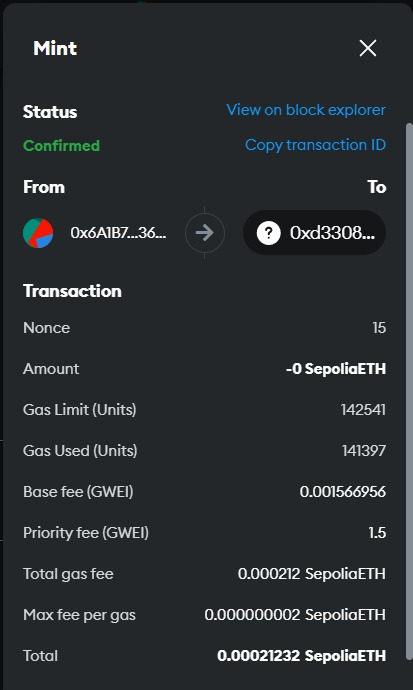
\includegraphics[scale=0.35]{gambar/riwayat_transaksi.jpeg}}
    % Keterangan gambar yang diinputkan
    \caption{Riwayat transaksi minting pada Metamask Wallet}
    % Label referensi dari gambar yang diinputkan
    \label{fig:minting}
    \end{figure}

    \item \emph{User} A akan melakukan \emph{minting} pada NFT dengan menggunakan MetaMask wallet, yang terhubung langsung ke Ethereum \emph{blockchain} melalui jaringan \emph{Sepolia Testnet}. Transaksi \emph{minting} ini mengkonfirmasi kreasi token baru di \emph{blockchain}, yang dicatat dengan detail transaksi seperti nonce, gas limit, dan biaya transaksi yang terdiri dari base fee dan priority fee. Proses ini mencatat NFT sebagai aset digital yang unik di \emph{blockchain}, memberikan hak kepemilikan digital kepada User A. Transaksi semacam ini memastikan keamanan dan transparansi dalam pencatatan kepemilikan aset digital, sekaligus mengintegrasikan NFT ke dalam ekosistem yang lebih luas di mana aset ini dapat diperdagangkan atau digunakan dalam aplikasi lain di masa depan.


    \item Tambahan dari gambar \ref*{fig:detail_transaksi_etherscan}, detail pada Etherscan memperlihatkan informasi kunci dari transaksi NFT yang dilakukan. \emph{Transaction hash} yang ditampilkan berfungsi sebagai pengenal unik transaksi, menunjukkan keberhasilannya pada \emph{blockchain}. Tanggal dan waktu transaksi juga tercatat, memberikan data penting mengenai kapan transaksi tersebut terjadi. Token yang terlibat adalah tipe ERC-721, standar untuk NFT yang memungkinkan representasi unik aset digital di Ethereum. Transaksi ini mencerminkan proses \emph{minting}, di mana NFT baru dibuat dan terdaftar di \emph{blockchain}, dan kemudian dialihkan dari alamat nol (menunjukkan penciptaan) ke alamat pemilik baru, yang dalam kasus ini adalah akun pertama yang melakukan \emph{minting}. Selain itu, biaya transaksi atau \emph{gas fee} yang relatif rendah menandakan efisiensi dalam pemrosesan transaksi tersebut di jaringan.

    \begin{figure} [H] \centering
    % Nama dari file gambar yang diinputkan
    \frame{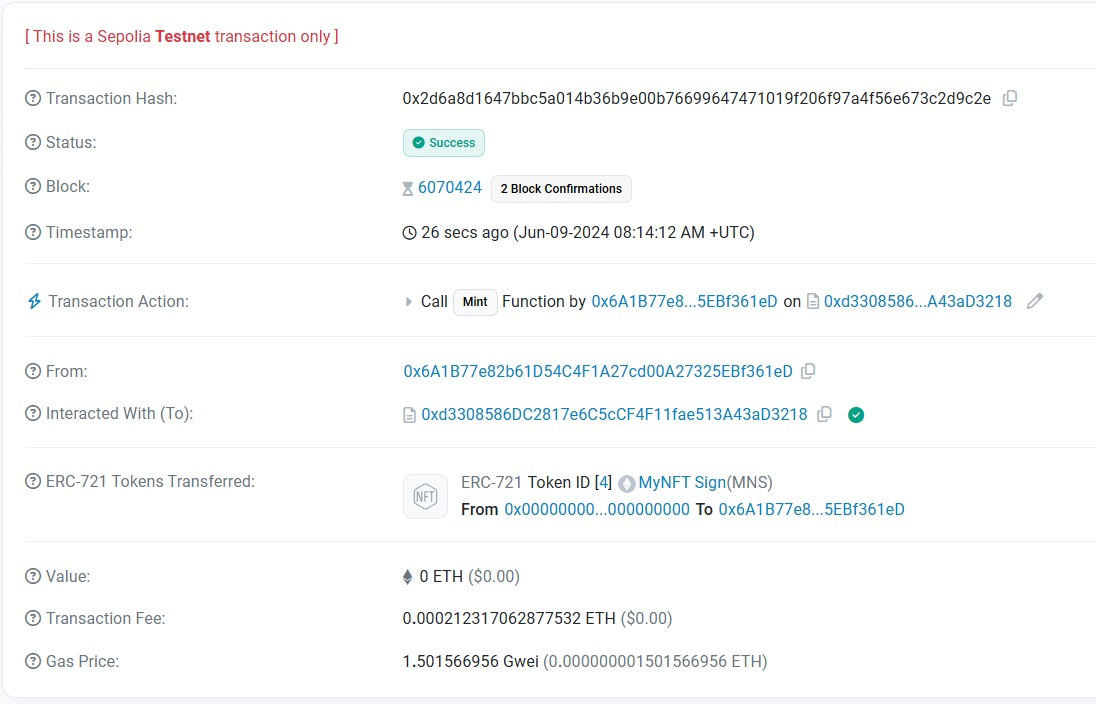
\includegraphics[scale=0.32]{gambar/detail_transaksi_etherscan.jpeg}}
    % Keterangan gambar yang diinputkan
    \caption{Detail transaksi pada Etherscan}
    % Label referensi dari gambar yang diinputkan
    \label{fig:detail_transaksi_etherscan}
    \end{figure}

    \item Pada gambar \ref*{fig:detail_nft_etherscan}, detail lebih lanjut mengenai NFT yang telah di-\emph{mint} juga dapat dilihat di Etherscan, seperti yang ditampilkan dalam gambar terlampir. Halaman Etherscan ini menyediakan data menyeluruh tentang NFT tersebut, termasuk alamat pemilik, alamat kontrak, dan pembuatnya. Setiap aspek dicatat dengan presisi untuk memastikan transparansi dan kemampuan dilacak dalam jaringan blockchain. Secara khusus, NFT ini, yang diidentifikasi sebagai "MyNFT Sign \#4", ditampilkan dengan ID token uniknya dan memastikan kepatuhan pada standar token ERC-721, yang menegaskan sifat non-fungible-nya. Tingkat detail ini penting untuk memverifikasi keaslian dan riwayat kepemilikan aset digital, membuat platform seperti Etherscan menjadi alat yang tak tergantikan dalam pengelolaan dan pertukaran NFT. Alat-alat ini juga meningkatkan keamanan transaksi digital dengan menyediakan jejak audit yang dapat diandalkan untuk setiap aset.

    \begin{figure} [H] \centering
    % Nama dari file gambar yang diinputkan
    \frame{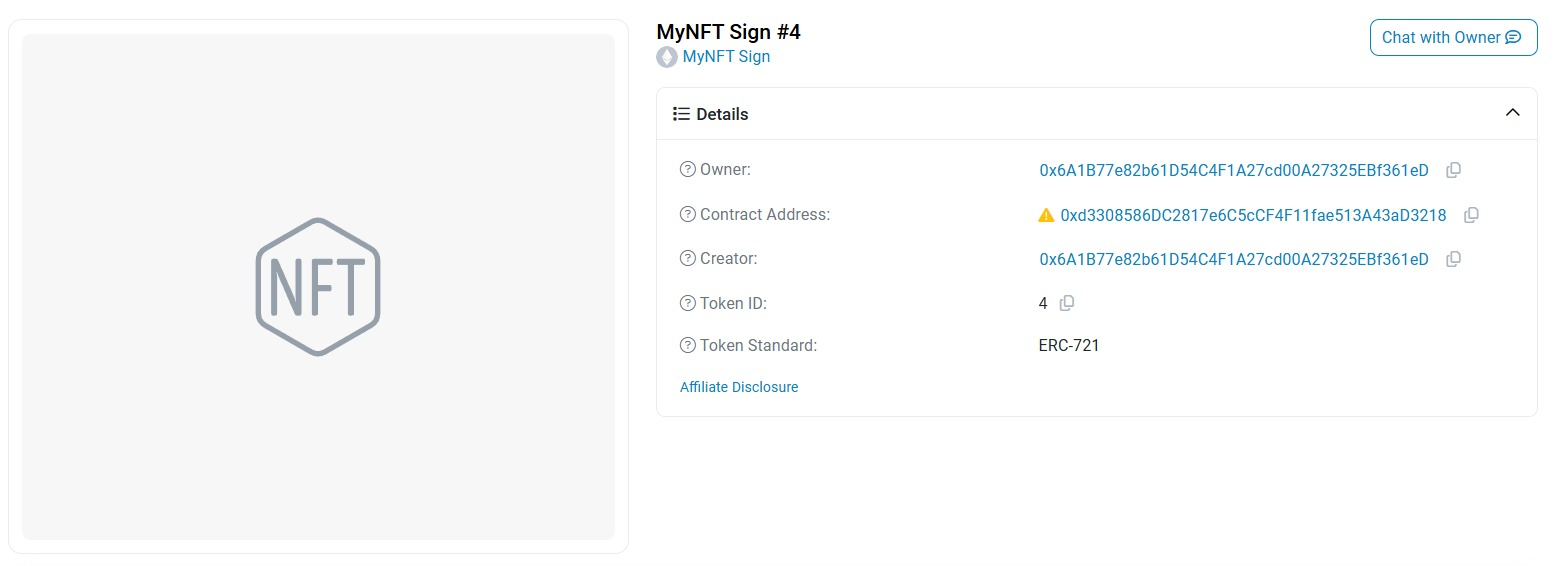
\includegraphics[scale=0.3]{gambar/detail_nft_etherscan.jpeg}}
    % Keterangan gambar yang diinputkan
    \caption{Detail NFT pada Etherscan}
    % Label referensi dari gambar yang diinputkan
    \label{fig:detail_nft_etherscan}
    \end{figure}
    
    \begin{figure} [H] \centering
    % Nama dari file gambar yang diinputkan
    \frame{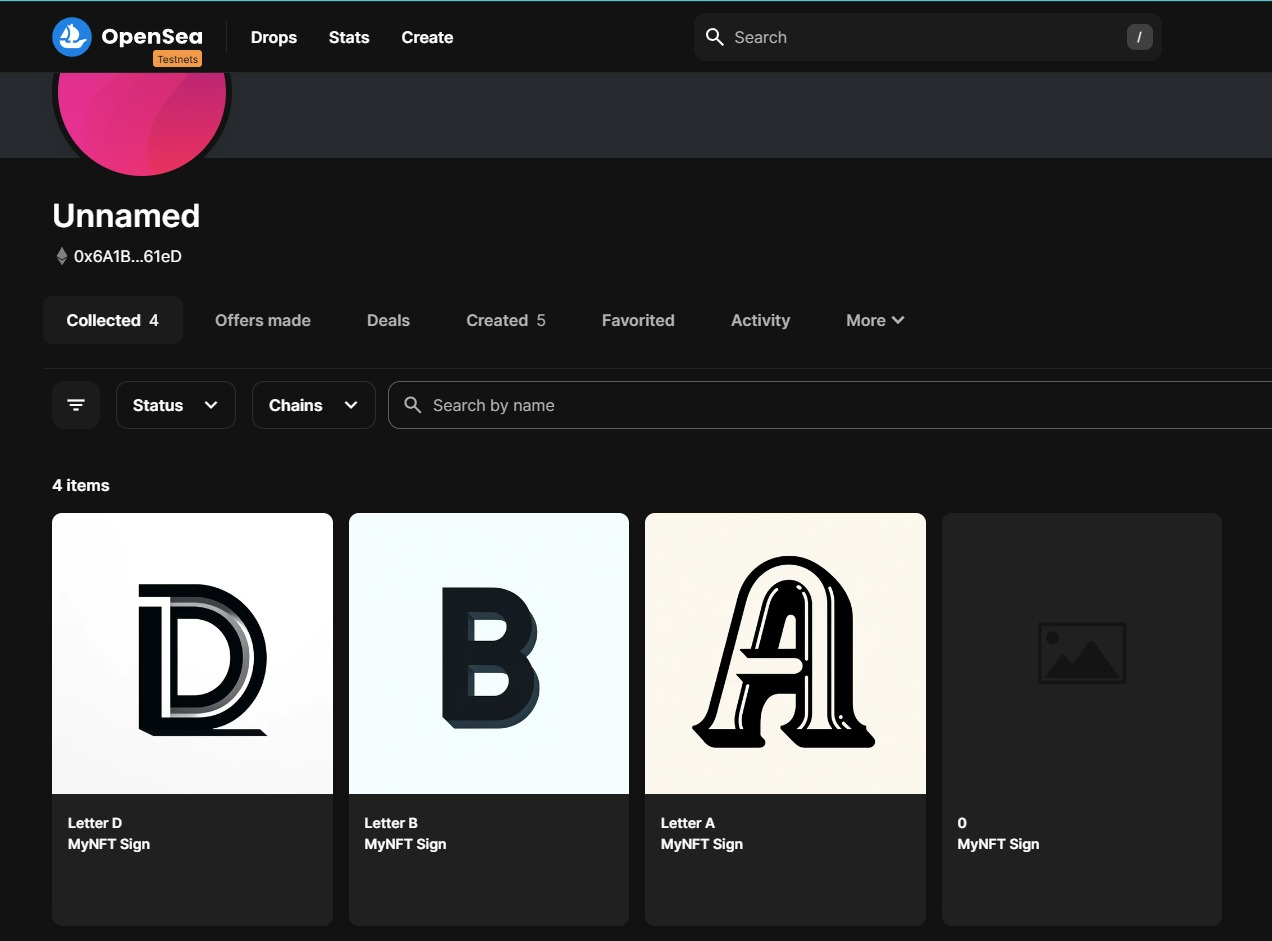
\includegraphics[scale=0.30]{gambar/nft_pada_opensea.jpeg}}
    % Keterangan gambar yang diinputkan
    \caption{NFT pada OpenSea}
    % Label referensi dari gambar yang diinputkan
    \label{fig:nft_opensea}
    \end{figure}

    \item Setelah proses \emph{minting} berhasil, seperti pada gambar \ref*{fig:nft_opensea} NFT yang telah di-\emph{minting} dapat dilihat pada platform OpenSea, yang merupakan pasar digital untuk aset kripto dan NFT. Dalam kasus pengujian ini, NFT yang telah di-minting adalah "Letter D", ditampilkan bersama dengan NFT lainnya yang telah dibuat oleh pengguna yang sama. Halaman OpenSea menampilkan berbagai detail seperti nama NFT, gambar, dan informasi lain yang relevan. Pengguna dapat melihat koleksi lengkap yang telah mereka mint atau beli. Setiap NFT ditampilkan dengan \emph{thumbnail} yang jelas, dan ketika di-klik, pengguna dapat melihat detail lebih lanjut seperti riwayat transaksi dan keaslian NFT tersebut. Ini memungkinkan pengguna untuk tidak hanya melihat koleksi mereka tetapi juga untuk berinteraksi dengan pasar, membuat penawaran, atau menjual NFT mereka.


    \item setelah NFT sudah terbuat, maka tahap berikutnya adalah melakukan \emph{lock} pada NFT yang akan dikirimkan ke \emph{user} B pada \emph{network} B'. Fungsi dari \emph{lock} ini untuk menjamin bahwa data token tidak diubah selama proses \emph{transfer}, menjaga kepercayaan dan keautentikan data NFT. Kemudian juga berguna untuk memberi sinyal kepada semua pihak terkait (pengguna, \emph{smart contract} di jaringan lain) bahwa token tersebut sedang dalam proses \emph{transfer}, dan operasi pada token harus ditangguhkan hingga proses selesai.

    \begin{figure} [H] \centering
    % Nama dari file gambar yang diinputkan
    \frame{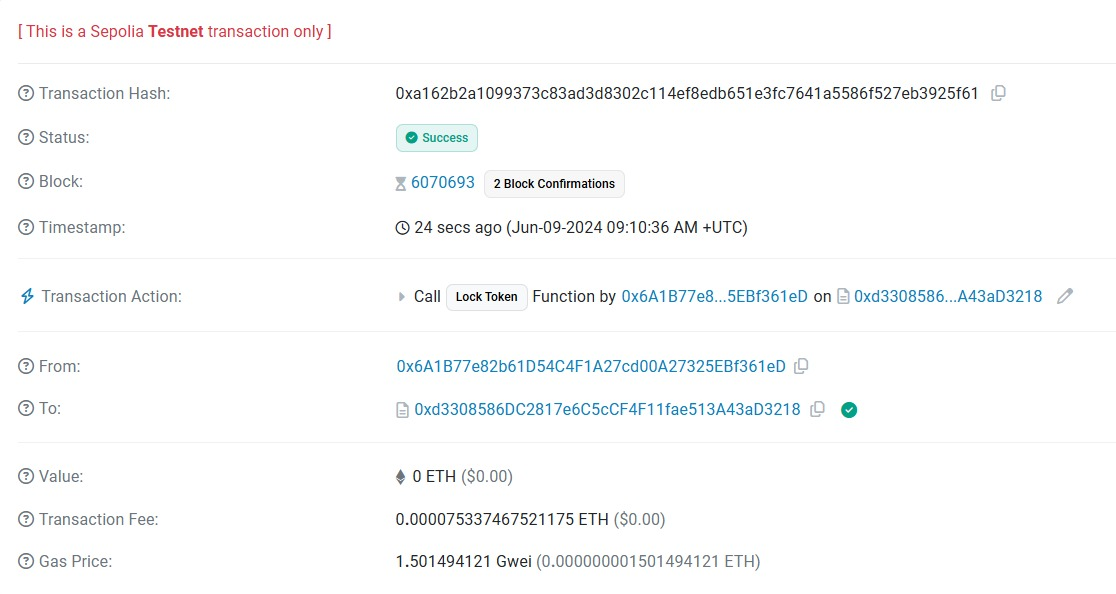
\includegraphics[scale=0.35]{gambar/lock_token.jpeg}}
    % Keterangan gambar yang diinputkan
    \caption{Detail fungsi \emph{Lock Token} pada Etherscan}
    % Label referensi dari gambar yang diinputkan
    \label{fig:locktoken}
    \end{figure}

    \item selesai melakukan proses \emph{lock token}, lalu fungsi \emph{bridge transfer} dapat dilaksanakan. Fungsi ini memfasilitasi transfer aman NFT antar \emph{blockchain} dengan memastikan bahwa NFT tersebut terkunci selama proses transfer dan memberikan visibilitas transparan tentang kejadian transfer melalui \emph{event} yang dicatat. Ini adalah komponen kunci dalam membangun aplikasi \emph{interoperable} yang memungkinkan aset \emph{digital} bergerak lintas ekosistem \emph{blockchain}.

    \begin{figure} [H] \centering
    % Nama dari file gambar yang diinputkan
    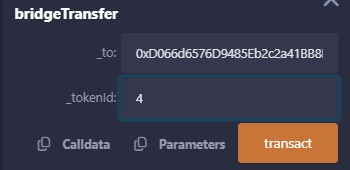
\includegraphics[scale=0.75]{gambar/bridge_transfer.jpeg}
    % Keterangan gambar yang diinputkan
    \caption{Parameter \emph{bridge transfer}}
    % Label referensi dari gambar yang diinputkan
    \label{fig:bridge_tranfer}
    \end{figure}

    \item pada gambar \ref{fig:bridge_tranfer} terdapat 2 parameter yaitu \texttt{"\emph{\_to}"}" yang digunakan untuk menerima parameter \emph{address} dari \emph{user} B dan juga parameter \texttt{"\emph{\_tokenId}"} untuk menerima argumen dari token NFT. Setelah dilakukan \emph{transact} maka akan dilanjutkan ke pembayaran pada Metamask Wallet.

    \begin{figure} [H] \centering
    % Nama dari file gambar yang diinputkan
    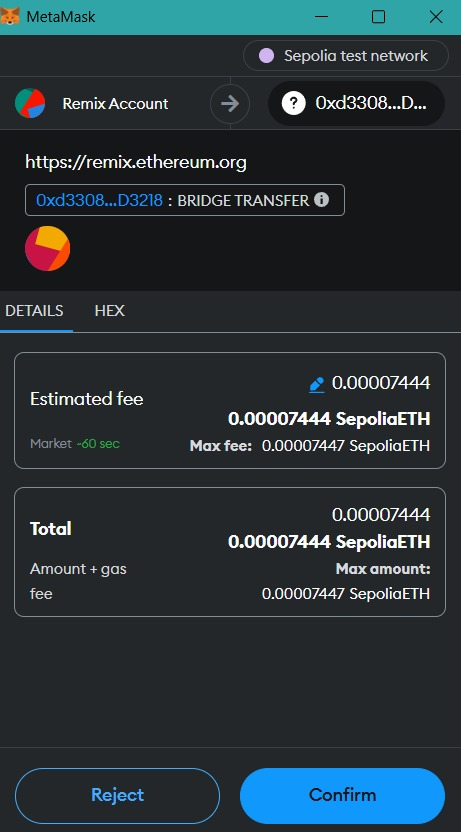
\includegraphics[scale=0.32]{gambar/verifikasi_metamask_wallet.jpeg}
    % Keterangan gambar yang diinputkan
    \caption{Pembayaran pada Metamask Wallet}
    % Label referensi dari gambar yang diinputkan
    \label{fig:metamask_pembayaran}
    \end{figure}

    \item setelah transaksi berhasil, \emph{record} dari transaksi tersimpan pada \emph{blockchain} yang dapat dilihat pada etherscan seperti pada gambar di bawah ini.

    \begin{figure} [H] \centering
    % Nama dari file gambar yang diinputkan
    \frame{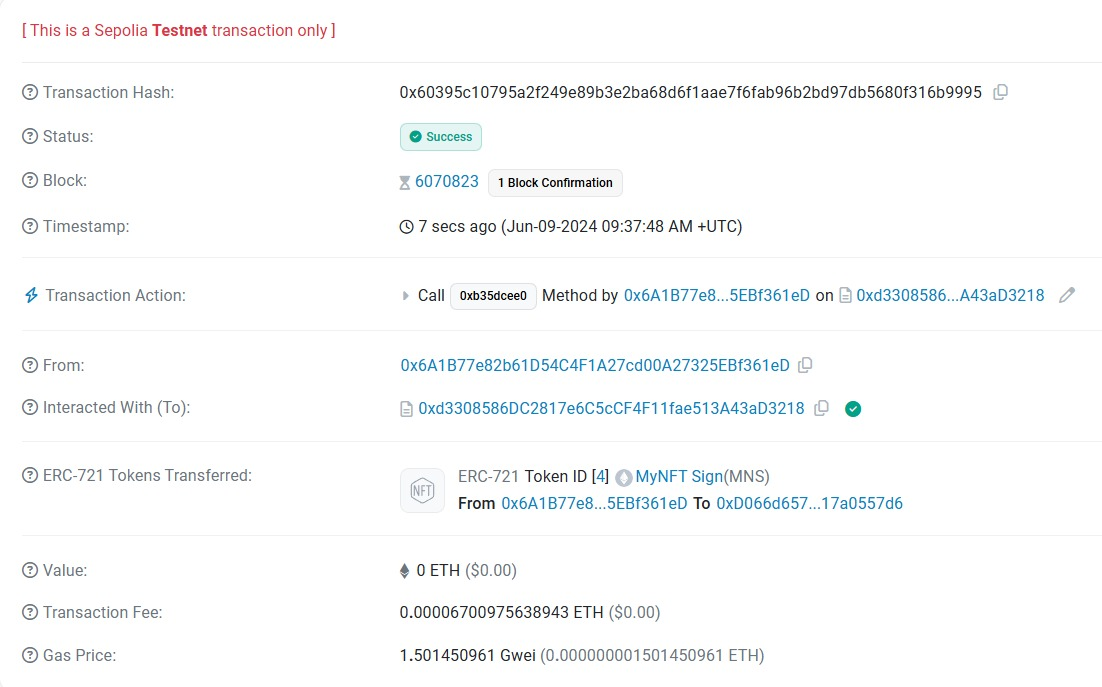
\includegraphics[scale=0.35]{gambar/detail_pada_etherscan.jpeg}}
    % Keterangan gambar yang diinputkan
    \caption{Detail pada Etherscan}
    % Label referensi dari gambar yang diinputkan
    \label{fig:detail_etherscan}
    \end{figure}

    \item pada etherscan juga terdapat detail pada NFT yang dapat dicek kepemilikannya. Jika dilihat dari gambar \ref{fig:detail_nft_etherscan} \emph{owner} dari NFT \#4 adalah \emph{address} dari \emph{user} A yang berada pada \emph{network Sepolia Ethereum Testnet}, lalu pada gambar di bawah ini setelah berhasil melakukan \emph{bridge transfer} kepemilikannya berganti kepada \emph{user} B yang berada pada \emph{network BNB Chain Testnet}.

    \begin{figure} [H] \centering
    % Nama dari file gambar yang diinputkan
    \frame{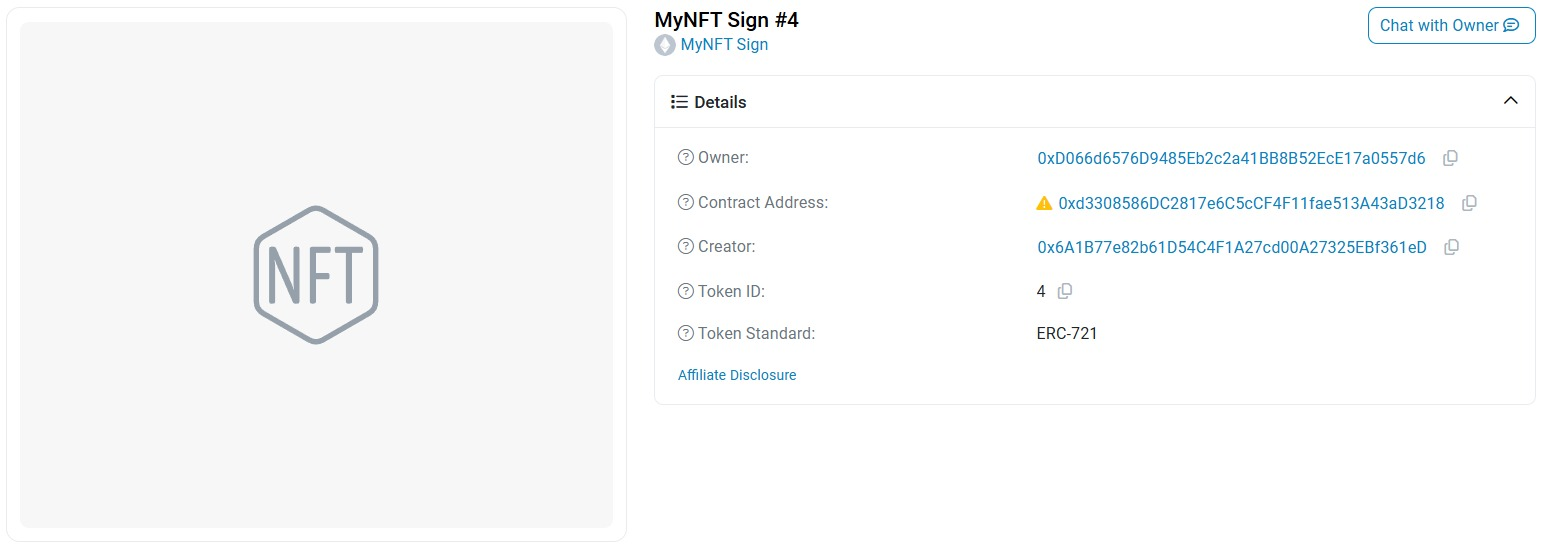
\includegraphics[scale=0.3]{gambar/nft_detail_etherscan2.jpeg}}
    % Keterangan gambar yang diinputkan
    \caption{Detail NFT pada Etherscan setelah \emph{bridge transfer}}
    % Label referensi dari gambar yang diinputkan
    \label{fig:nft_bridge_transfer}
    \end{figure}

    \item pada \emph{platform} OpenSea juga dapat dilihat pada akun milik \emph{adrress} \emph{user} B maka juga terdapat NFT yang telah terkirim ke alamatnya.

    \begin{figure} [H] \centering
    % Nama dari file gambar yang diinputkan
    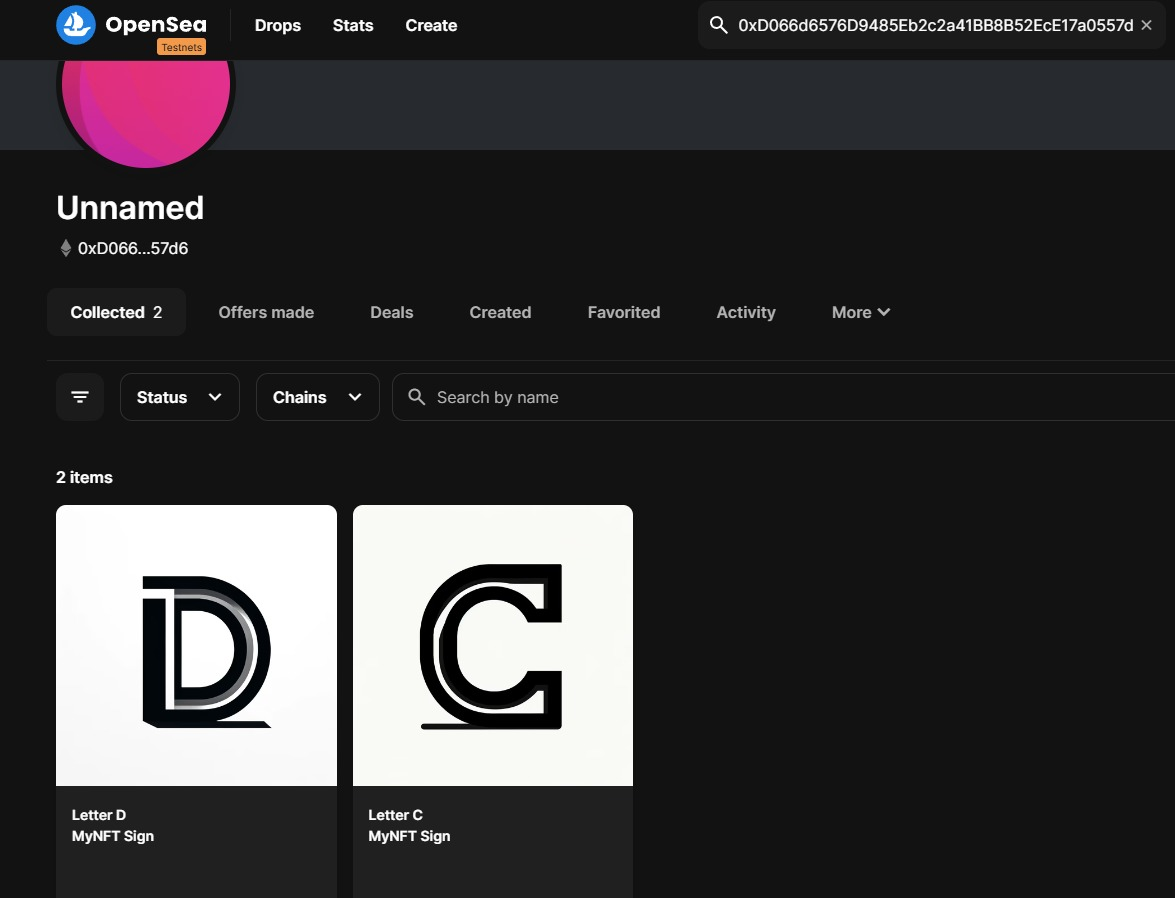
\includegraphics[scale=0.27]{gambar/nft_pada_opensea_2.jpeg}
    % Keterangan gambar yang diinputkan
    \caption{NFT pada OpenSea \emph{address} B}
    % Label referensi dari gambar yang diinputkan
    \label{fig:opensea2}
    \end{figure}
    
\end{itemize}

\subsection{Pengujian Integrasi \emph{Smart Contract} Dengan Web3.0}
Ekspektasi pengujian dari integrasi sistem \emph{smart contract} dengan web3.0 antara lain adalah sebagai berikut:
\begin{itemize}
    \item \emph{User} dapat melakukan integrasi akun Metamask Wallet dengan aplikasi web3.0

    \item \emph{User} dapat melakukan \emph{create listing} NFT untuk mengunggah NFT dari pemilik ke halaman \emph{Home} dan ke halaman \emph{My Listed Items}.

    \item \emph{User} dapat melakukan minting pada NFT yang telah dibuat dan kemudian terlihat pada halaman \emph{My Purchases}.

    \item \emph{User} yang memiliki NFT tersebut dapat melakukan \emph{transfer ownership} atau pindah kepemilikan dari alamat pengguna pemilik menuju ke alamat pengguna tujuan.

    \item \emph{User} yang memiliki NFT tersebut dapat melakukan fungsi seperti tahapan dalam melakukan \emph{bridge transfer} untuk melakukan pengiriman NFT dari alamat pengguna pada \emph{network} lokal ke alamat pengguna tujuan yang berada pada \emph{network} \emph{binance smart chain} ataupun \emph{sepolia ethereum}. 
\end{itemize}

Berikut merupakan langkah-langkah dari pengujian integrasi \emph{smart contract} dengan Web3.0 yang akan dilakukan:

\begin{itemize}
    \item \emph{User} akan mengakses web dengan menggunakan link yang dimunculkan secara lokal dengan melakukan run program lalu akan memunculkan link berupa \emph{localhost} yang dapat diakses pada platform seperti Google Chrome, Mozilla Firefox, atau Microsoft Edge, dan platform pengakses website lainnya.

    \begin{figure} [H] \centering
      % Nama dari file gambar yang diinputkan
      \frame{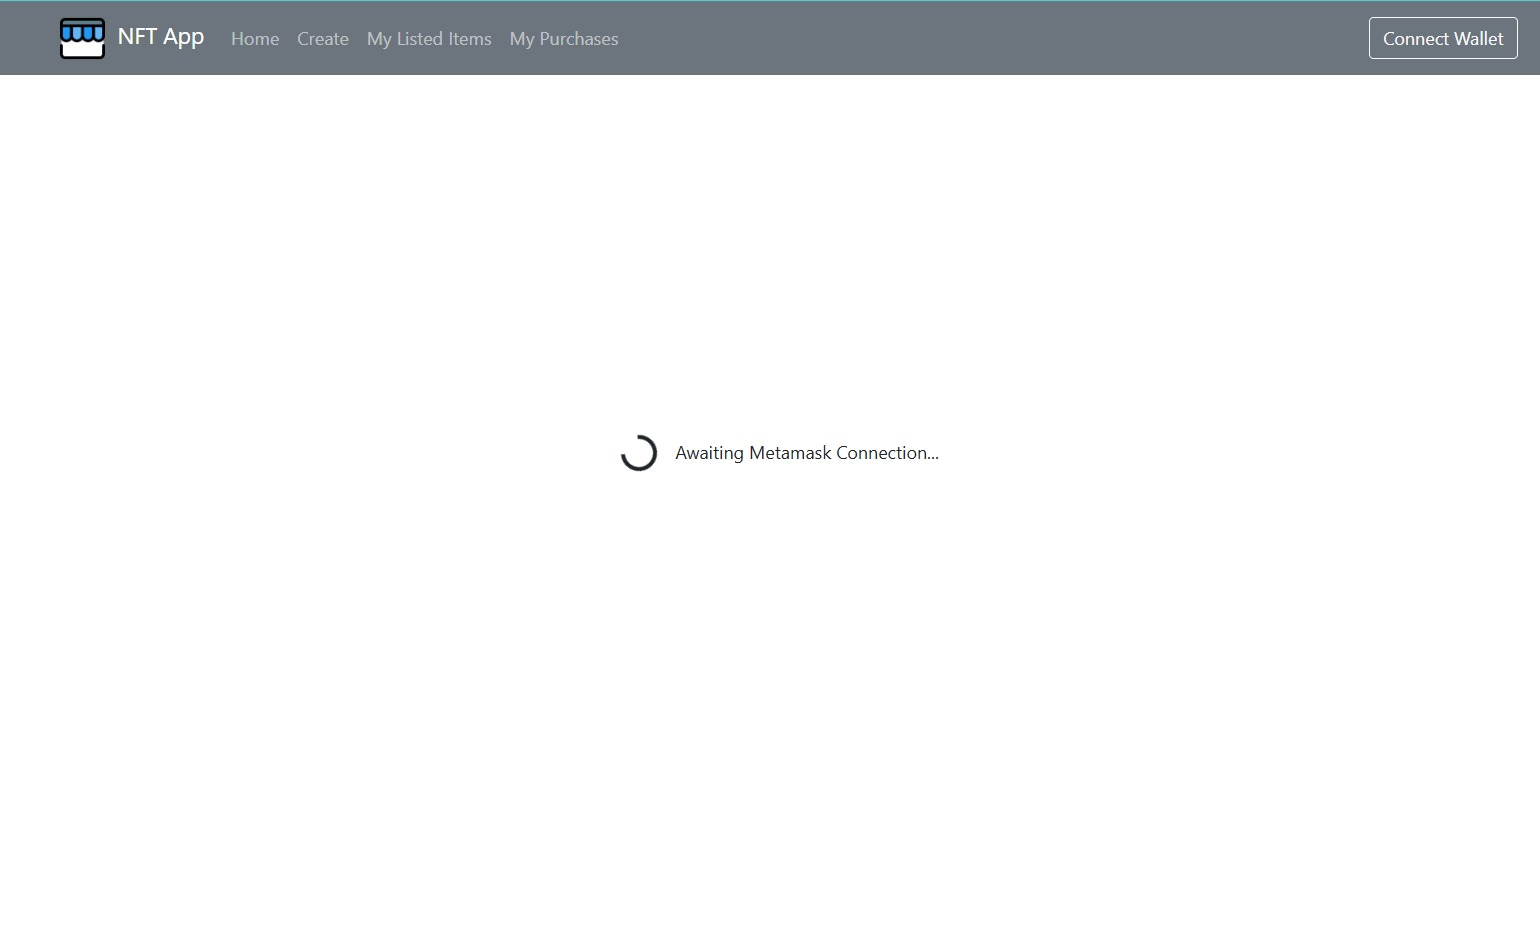
\includegraphics[scale=0.26]{gambar/login_page.jpg}}
      % Keterangan gambar yang diinputkan
      \caption{Tampilan awal dari web}
      % Label referensi dari gambar yang diinputkan
      \label{fig:web_interface}
      \end{figure}

    \item Pada gambar \ref{fig:web_interface} merupakan tampilan utama dari web, sebelum dapat melakukan \emph{load} data pengguna harus melakukan koneksi dengan akun Metamask Wallet. Integrasi harus dilakukan agar pengguna dapat mengakses tampilan lanjutan pada web. Integrasi tersebut dapat dilakukan dengan menekan tombol \emph{Connect Wallet} pada \emph{navigation bar} di pojok kanan atas.
    
    \begin{figure} [H] \centering
      \centering
      \begin{subfigure}{0.45\textwidth}
          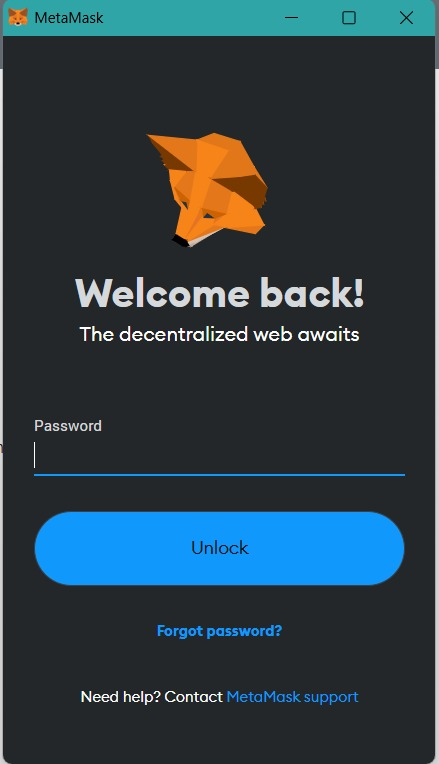
\includegraphics[scale=0.35]{gambar/integrasi_metamask.jpg}
          \caption{}
          \label{fig:intg_a}
      \end{subfigure}
      \hspace{5pt}
      \begin{subfigure}{0.45\textwidth}
        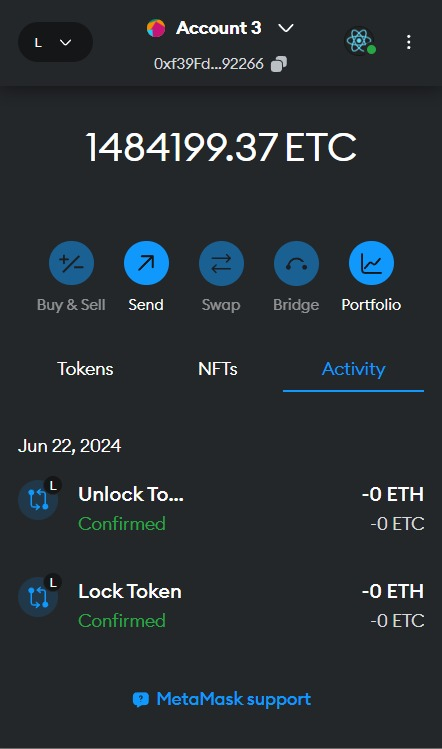
\includegraphics[scale=0.35]{gambar/metamask_konek.jpeg}
        \caption{}
        \label{fig:intg_b}
    \end{subfigure}
      \caption{Koneksi Metamask dengan Web}
      \label{fig:koneksi_web_metamask}
      \end{figure}

      \item Pada gambar \ref{fig:koneksi_web_metamask} adalah proses ketika melakukan integrasi dengan Metamask Wallet pada web. Ketika pengguna menekan tombol \emph{Connect Wallet} maka akan diarahkan kepada Metamask. Jika pengguna belum melakukan login pada Metamask maka pengguna akan disuruh login terlebih dahulu pada Metamask seperti pada gambar \ref{fig:intg_a}. Jika pengguna telah melakukan login ke akun Metamask, maka tampilannya akan seperti gambar \ref{fig:intg_b} yang di mana tampilan dari Metamask Wallet terdapat informasi \emph{address} dari akun dan juga \emph{balance} dari akun tersebut. Dikarenakan pada pengujian ini masih menggunakan \emph{localhost} maka \emph{balance} dari akun tersebut menggunakan milik Hardhat.
        
        \item Kemudian, kita akan menguji fungsionalitas sistem dengan fokus pada proses pengunggahan NFT, melakukan transaksi pembelian, serta mengirim NFT ke \emph{address} lain. Dalam skenario pengujian ini, seluruh aktivitas akan dilakukan dalam jaringan yang sama, yakni \emph{localhost}. Hal ini bertujuan untuk memastikan bahwa interaksi antar fungsi dalam \emph{smart contract} berjalan dengan lancar dan tanpa adanya gangguan eksternal yang mungkin terjadi dalam jaringan publik. Pengujian di \emph{localhost} memungkinkan kita untuk mengisolasi dan mengidentifikasi masalah fungsi dalam kondisi yang terkontrol sebelum memindahkannya ke jaringan tes yang lebih besar atau ke jaringan Ethereum utama. Selama proses ini, kita akan mengamati bagaimana sistem menangani proses-proses seperti penentuan kepemilikan, transaksi pembayaran, dan transfer kepemilikan antar pengguna, yang semuanya merupakan komponen penting dari aplikasi berbasis NFT. Pengujian ini juga mencakup verifikasi keamanan dan integritas data untuk memastikan bahwa tidak ada celah yang dapat dimanfaatkan oleh pengguna jahat dalam ekosistem.
      
      \begin{figure} [H] \centering
        % Nama dari file gambar yang diinputkan
        \frame{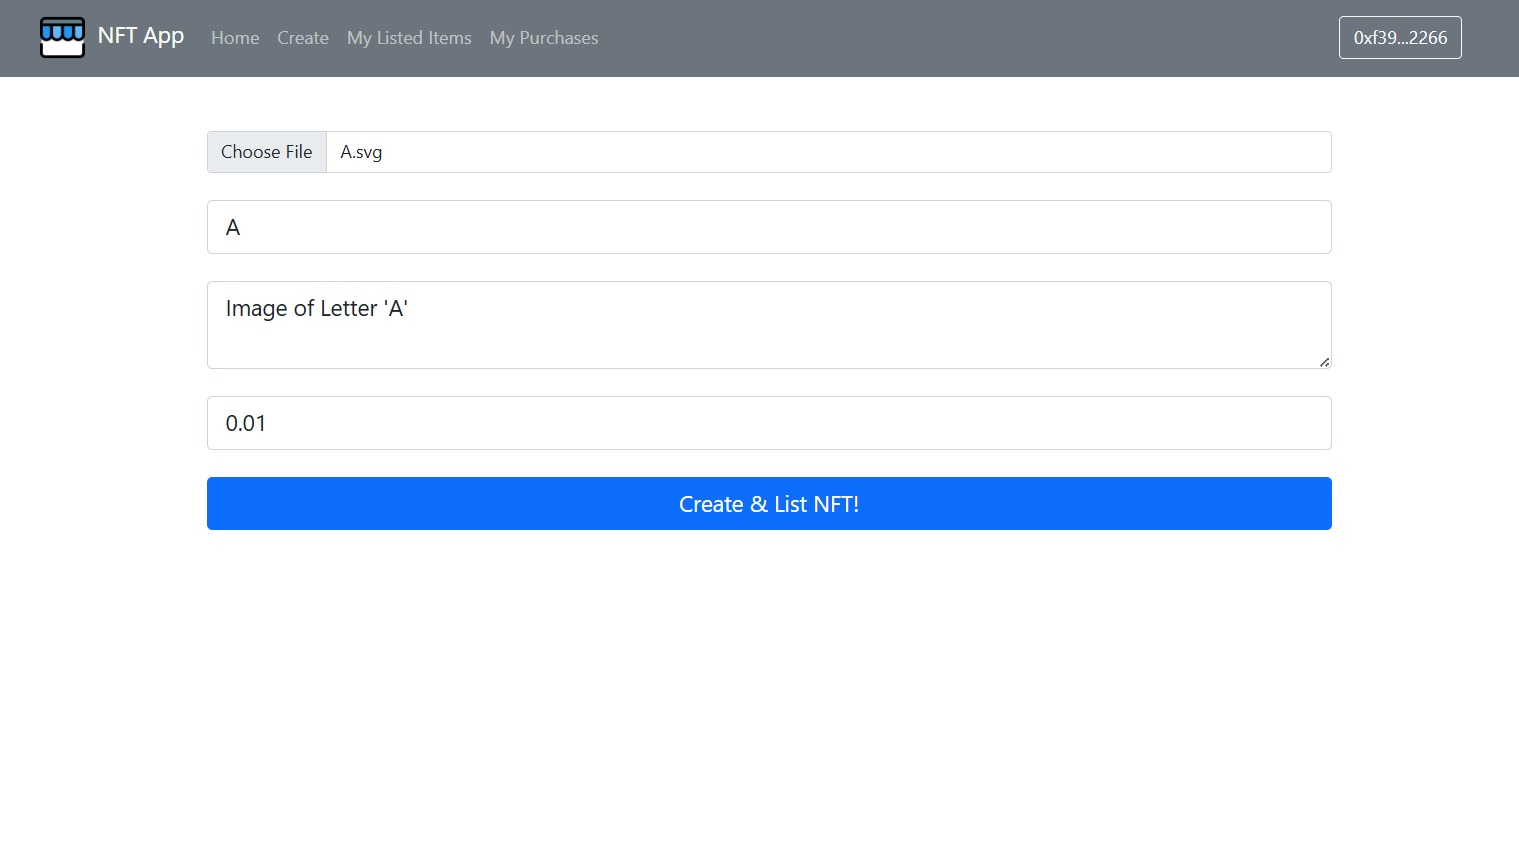
\includegraphics[scale=0.27]{gambar/create_nft.jpg}}
        % Keterangan gambar yang diinputkan
        \caption{Melakukan pengunggahan NFT pada halaman \emph{create}}
        % Label referensi dari gambar yang diinputkan
        \label{fig:createnft}
        \end{figure}

      \item Pada tahap awal ini pengguna melakukan pengunggahan NFT pada halaman \emph{create}. Pengguna memasukkan detail-detail dari NFT yang ingin diunggah seperti gambar, nama, deskripsi, dan juga harga dalam mata uang \emph{ethereum}. Pada pengujian ini pengguna memasukkan NFT gambar "A" seperti pada pengujian \emph{smart contract} sebelumnya. Setelah pengguna menekan tombol "\emph{Create \& List NFT!}" maka akan muncul \emph{pop up window} dari Metamask Wallet yang digunakan untuk membayar \emph{gas} atau fee dari melakukan eksekusi kode \emph{smart contract}. 
      
       \begin{figure} [H] \centering
      \centering
      \begin{subfigure}{0.45\textwidth}
          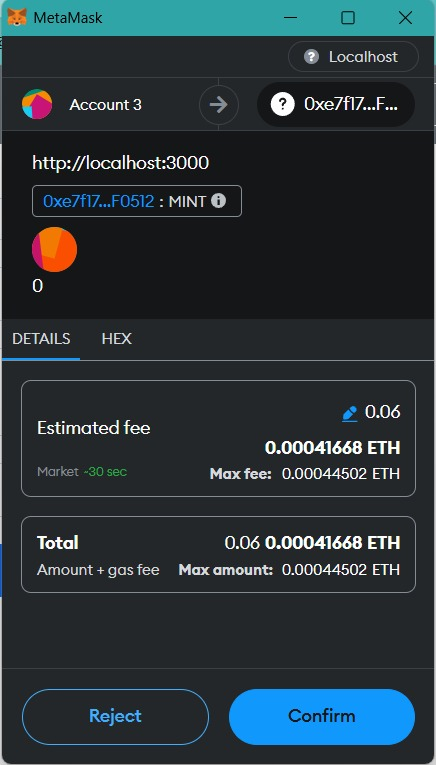
\includegraphics[scale=0.32]{gambar/confirm_create.jpg}
          \caption{}
          \label{fig:payipfs-a}
      \end{subfigure}
      \hspace{5pt}
      \begin{subfigure}{0.45\textwidth}
        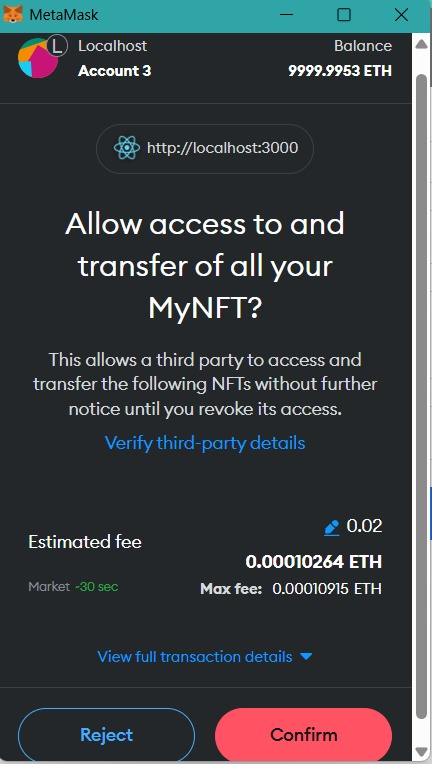
\includegraphics[scale=0.32]{gambar/confirm_upload.jpg}
        \caption{}
        \label{fig:payipfs-b}
    \end{subfigure}
      \caption{Pembayaran gas IPFS menggunakan Metamask Wallet}
      \label{fig:koneksi_web_metamask}
      \end{figure}
      
        \item Gambar \ref{fig:payipfs-a} adalah pembayaran \emph{gas} dari metamask wallet. Pembayaran \emph{gas} tersebut terjadi karena pada \emph{smart contract} terjadi proses pengunggahan gambar NFT ke platform penyedia IPFS. Pada web ini kita mengintegrasikan dengan platform bernama Pinata. Pinata sendiri merupakan platform penyedia servis IPFS. Kemudian juga terdapat konfirmasi pada gambar \ref{fig:payipfs-b}, konfirmasi ini dilakukan karena melakukan integrasi dengan platform Pinata yang kita gunakan sebagai penyedia servis IPFS. 
        
        \item Setelah berhasil melakukan konfirmasi pembayaran gas melalui MetaMask, NFT yang telah dibuat melalui halaman "Create" pada aplikasi akan diunggah ke platform Pinata. Platform Pinata ini berfungsi sebagai penyedia layanan penyimpanan dan pengelolaan file berbasis teknologi blockchain, yang menggunakan sistem InterPlanetary File System (IPFS) untuk memastikan keamanan dan ketahanan data.
        
        \begin{figure} [H] \centering
          % Nama dari file gambar yang diinputkan
          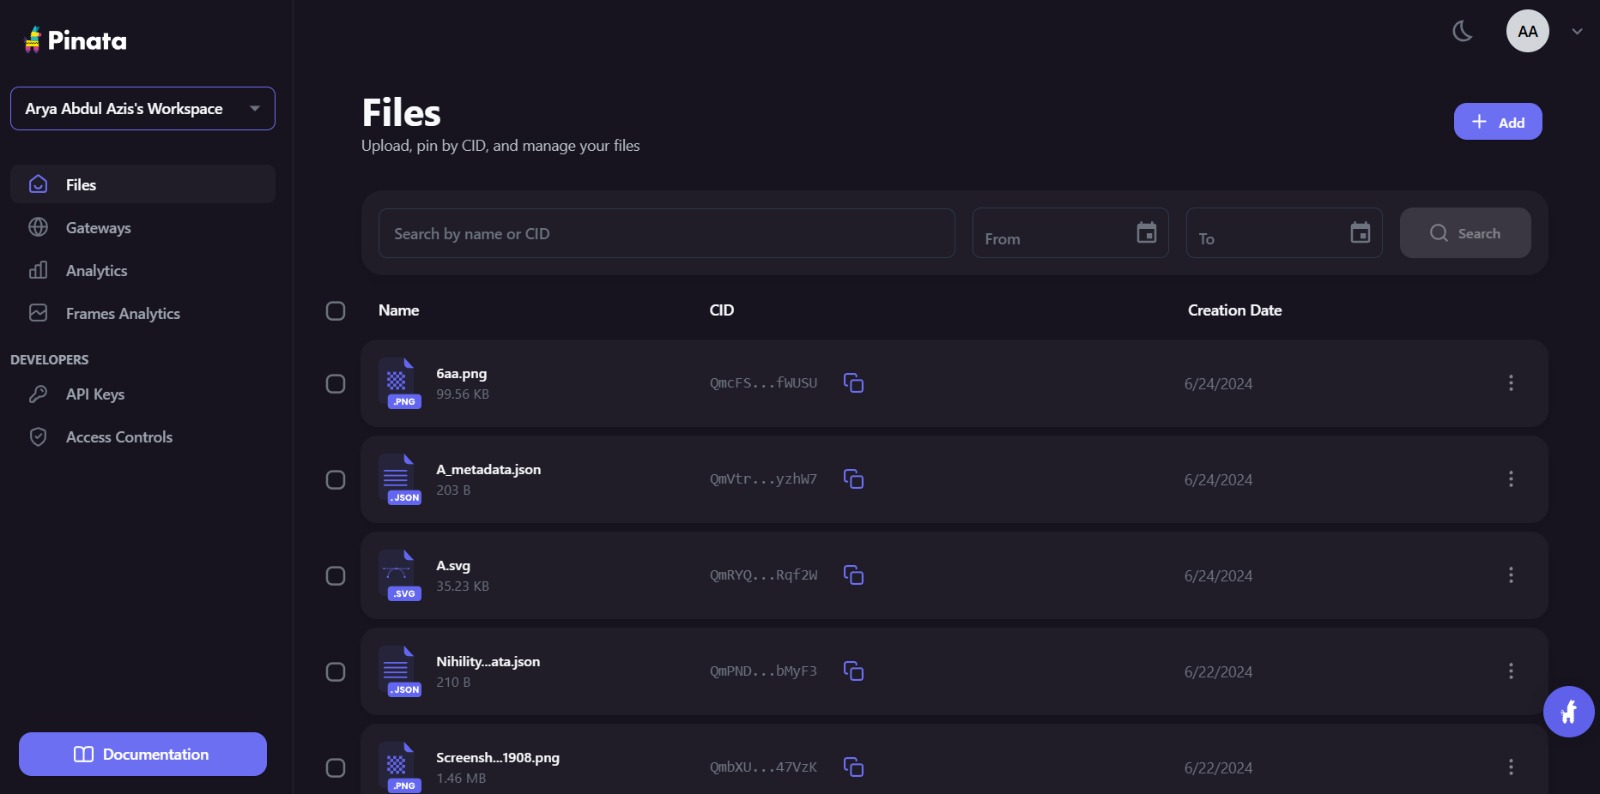
\includegraphics[scale=0.25]{gambar/pinata.jpeg}
          % Keterangan gambar yang diinputkan
          \caption{Data dari NFT ter-\emph{upload} pada platform Pinata}
          % Label referensi dari gambar yang diinputkan
          \label{fig:pinata}
          \end{figure}

        \item Dalam platform Pinata seperti pada gambar \ref{fig:pinata}, setiap file yang diunggah, termasuk gambar untuk NFT, akan diberikan Content Identifier (CID) unik yang memudahkan pelacakan dan akses tanpa perlu mengkhawatirkan perubahan isi file, karena CID ini akan berubah jika konten file berubah. Hal ini sangat penting dalam ekosistem NFT di mana keaslian dan keunikan konten harus terjamin. Di Pinata, pengguna dapat dengan mudah melihat semua file yang telah diunggah, mengatur akses, dan memantau penggunaan dan analisis lalu lintas file. Fitur ini memungkinkan pembuat konten NFT untuk tidak hanya menyimpan aset digital mereka dengan aman tetapi juga mengelola distribusi mereka dengan lebih efektif dalam pasar digital. Keseluruhan proses ini mengintegrasikan teknologi blockchain dengan aplikasi web, memastikan bahwa setiap pembelian dan transfer NFT dapat dilacak dan diverifikasi secara transparan dan aman. Pinata tidak hanya menyediakan solusi penyimpanan yang efisien dan aman tetapi juga menawarkan antarmuka yang ramah pengguna, memudahkan para pengguna, terutama para pembuat NFT, untuk mengunggah dan mengelola aset digital mereka dengan mudah. Fitur pencarian dan pengelolaan file yang intuitif memungkinkan pengguna untuk mengakses dan mengatur koleksi NFT mereka tanpa hambatan, memastikan bahwa aset digital dapat dikelola dan diakses dengan cepat sesuai kebutuhan. Lebih lanjut, Pinata mendukung integrasi dengan berbagai platform dan marketplace NFT, sehingga memperluas jangkauan dan visibilitas aset digital yang disimpan di dalamnya. Hal ini memberikan nilai tambah bagi para pembuat dan kolektor NFT dalam mendistribusikan dan memperdagangkan karya mereka di berbagai platform dengan mudah dan aman. Melalui Pinata, pembuat NFT dapat memastikan bahwa setiap aset digital tidak hanya aman tetapi juga siap untuk diintegrasikan dan digunakan dalam ekosistem blockchain yang lebih luas.
      
        \begin{figure} [H] \centering
          % Nama dari file gambar yang diinputkan
          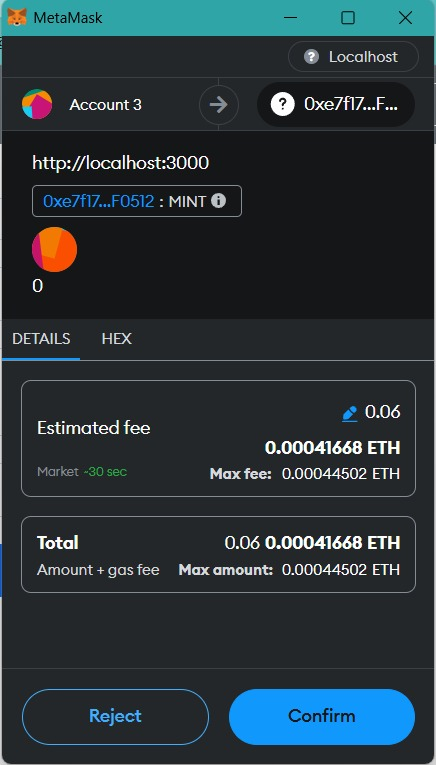
\includegraphics[scale=0.43]{gambar/confirm_create.jpg}
          % Keterangan gambar yang diinputkan
          \caption{Melakukan konfirmasi \emph{minting} NFT pada Metamask Wallet}
          % Label referensi dari gambar yang diinputkan
          \label{fig:makenft}
          \end{figure}
      
      \item 
      Pada gambar \ref{fig:makenft}, ditampilkan jendela konfirmasi MetaMask yang digunakan untuk memberikan persetujuan atas transaksi minting NFT. Dalam jendela ini, pengguna diminta untuk mengkonfirmasi atau menolak transaksi yang sedang diinisiasi dari aplikasi yang dihosting pada localhost:3000. Proses ini memastikan bahwa pengguna memahami dan menyetujui semua detail transaksi sebelum melanjutkan. Di dalam jendela konfirmasi, jumlah ETH yang akan ditransfer adalah 0, yang menandakan bahwa transaksi ini mungkin hanya melibatkan biaya gas, tanpa ada transfer dana tambahan yang terlibat. "Estimated fee" atau perkiraan biaya gas untuk transaksi ini ditampilkan, dengan jumlah minimal yang ditetapkan serta maksimum yang mungkin diperlukan, memberikan transparansi tentang biaya yang dapat dikeluarkan untuk memproses transaksi ini. Selain itu, MetaMask juga menyediakan informasi mengenai durasi estimasi untuk penyelesaian transaksi di pasar yang ditandai dengan "+30 sec", yang berarti transaksi diharapkan terjadi dalam waktu sekitar 30 detik.

      
      \begin{figure} [H] \centering
        % Nama dari file gambar yang diinputkan
        \frame{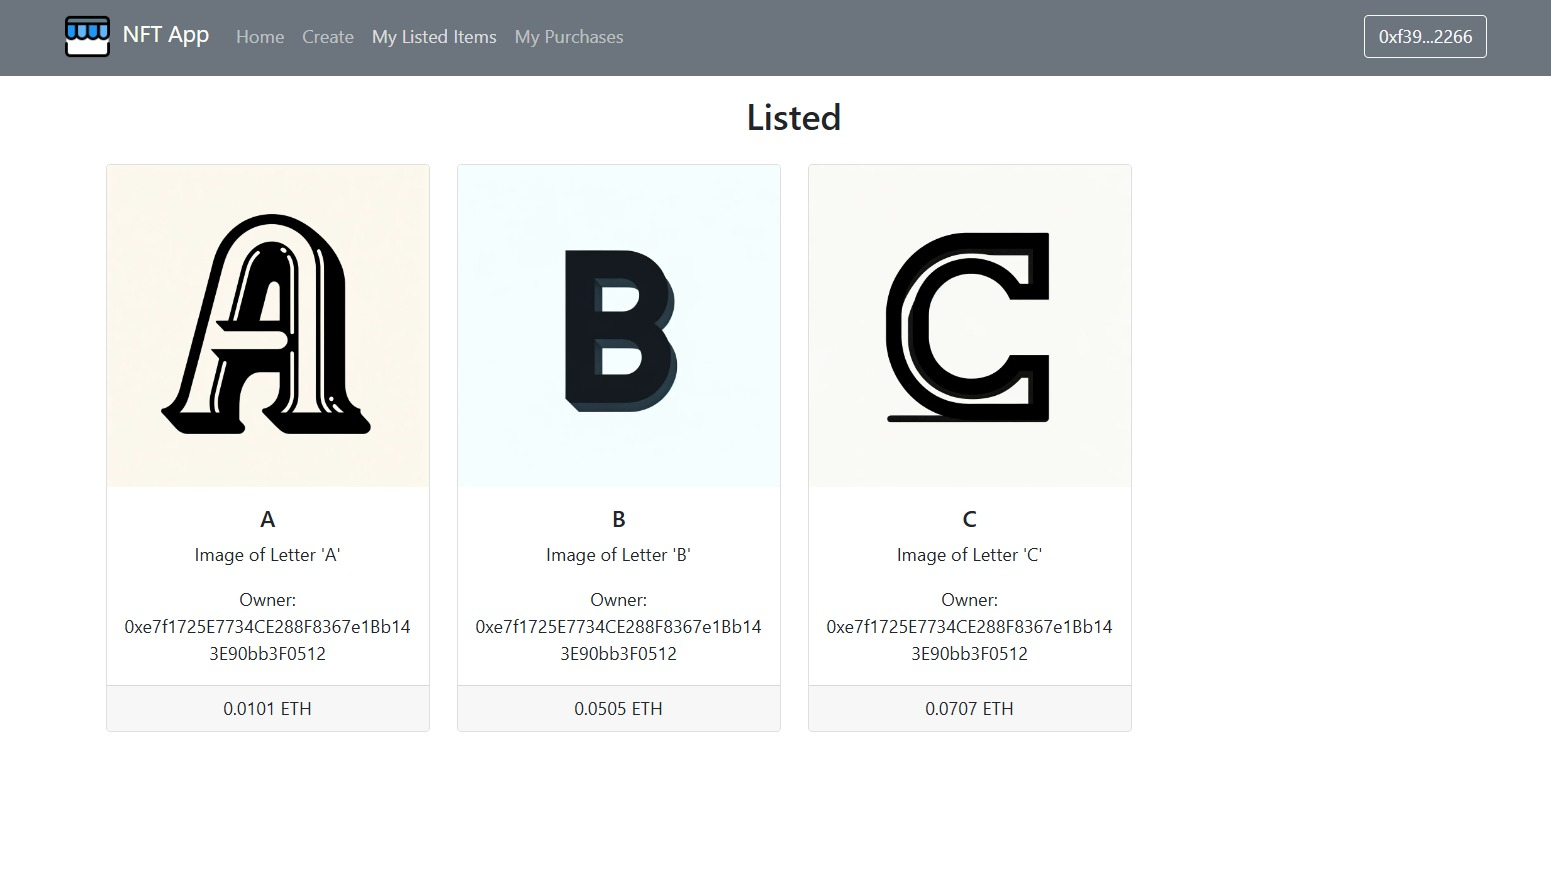
\includegraphics[scale=0.26]{gambar/listed_nft.jpeg}}
        % Keterangan gambar yang diinputkan
        \caption{NFT yang telah di-\emph{minting} terlihat pada halaman \emph{My listed items}}
        % Label referensi dari gambar yang diinputkan
        \label{fig:listeditem}
      \end{figure}

      \item Setelah pengguna menyelesaikan proses minting NFT dan melakukan konfirmasi melalui MetaMask seperti yang dijelaskan sebelumnya, NFT yang baru dibuat akan muncul pada halaman "My Listed Items" dalam aplikasi. Halaman ini berfungsi sebagai galeri pribadi pengguna dimana semua NFT yang telah mereka buat dan daftarkan untuk dijual ditampilkan. Dalam contoh yang ditampilkan pada gambar, NFT dengan desain huruf "A" yang telah berhasil di-\emph{list} tampak dengan harga yang tertera di bawah gambar yaitu 0.0101 ETH. Kemudian juga terdapat NFT dengan desain huruf "B" yang berhasil di-\emph{list} dengan harga yang tertera di gambar yaitu 0.0505 ETH, dan juga NFT dengan desain huruf "C" yang berhasil di-\emph{list} dengan harga yang tertera di gambar yaitu 0.0707 ETH. Hal ini menandakan bahwa NFT ini siap untuk dibeli oleh pengguna lain. Setiap NFT yang terdaftar di halaman ini akan menampilkan gambar yang berkaitan dengan NFT tersebut, yang merupakan hasil unggahan pengguna ke IPFS, dan metadata lainnya seperti nama dan deskripsi juga akan ditampilkan jika pengguna telah menyertakannya saat proses minting.
      
      \item Setelah menyelesaikan proses pengunggahan dan minting NFT, NFT yang baru dibuat juga dapat dilihat di halaman utama (\emph{home page}) web aplikasi NFT. Gambar yang disajikan menunjukkan NFT berupa gambar huruf "A", yang ditampilkan dengan label dan harga penjualan. Di halaman utama ini, NFT tidak hanya dipamerkan tetapi juga siap untuk dibeli oleh pengguna lain. Dalam tampilan ini, setiap NFT yang di-list akan dilengkapi dengan tombol "\emph{Buy}" yang memungkinkan pengguna langsung membeli NFT tersebut. Tombol ini memfasilitasi pembelian langsung tanpa perlu navigasi ke halaman lain, memberikan kemudahan bagi pembeli untuk segera mengakuisisi aset digital yang diinginkan. 

      \begin{figure} [H] \centering
        % Nama dari file gambar yang diinputkan
        \frame{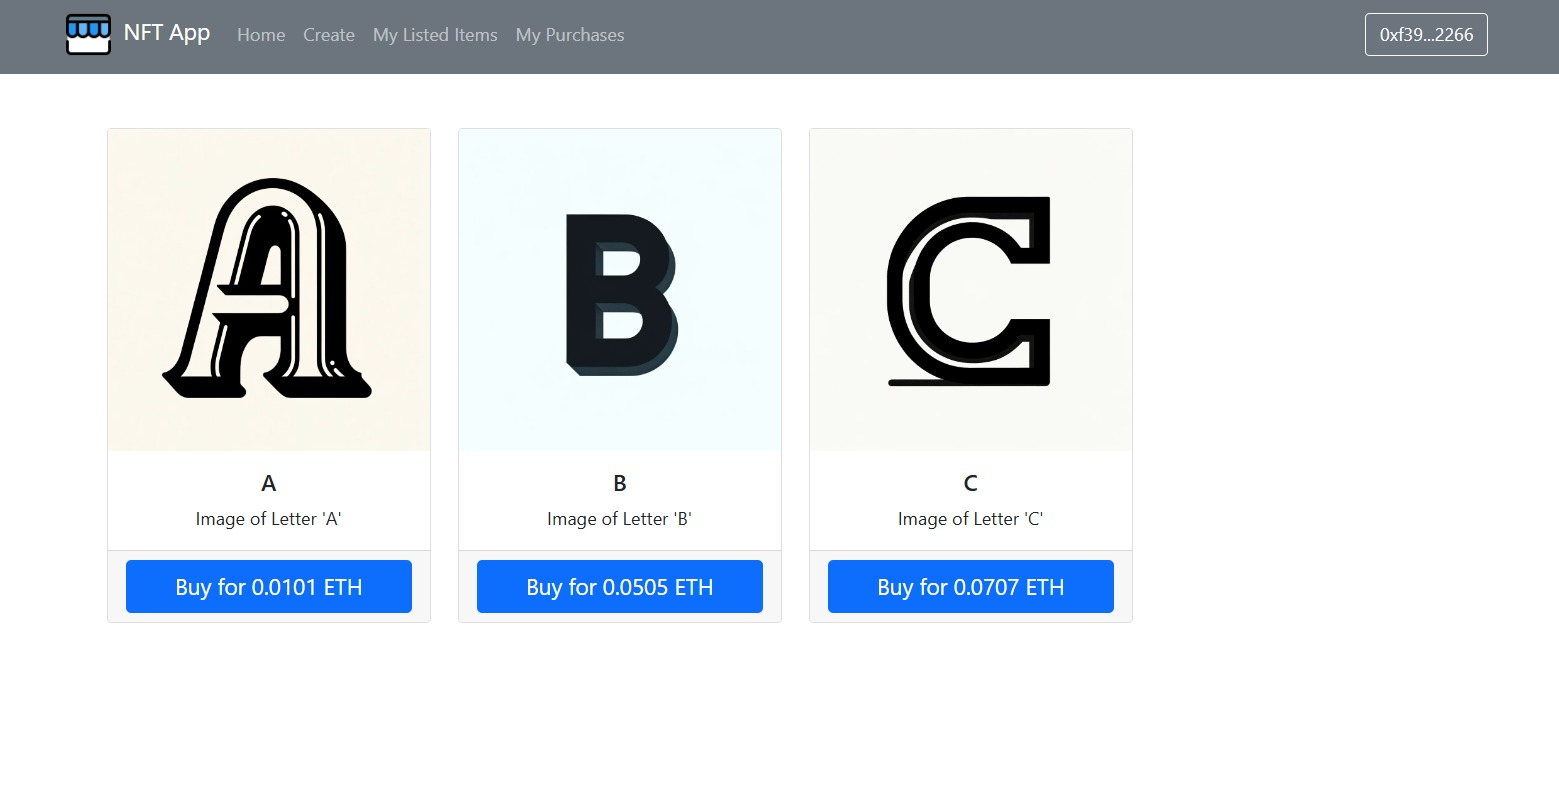
\includegraphics[scale=0.26]{gambar/nft_listed_home.jpeg}}
        % Keterangan gambar yang diinputkan
        \caption{NFT yang telah di-\emph{minting} terlihat pada halaman \emph{home}}
        % Label referensi dari gambar yang diinputkan
        \label{fig:listhome}
        \end{figure}

        \item Pada gambar \ref{fig:listhome} ketika tombol tersebut diklik, transaksi akan diproses melalui MetaMask atau wallet digital lainnya yang telah disinkronkan dengan aplikasi. Halaman ini dirancang untuk memberikan pengalaman pengguna yang intuitif dan efisien, di mana pembeli dapat dengan cepat mengakses NFT yang mereka inginkan dan melihat informasi penting seperti nama, deskripsi, dan harga NFT. Ini tidak hanya memperkuat transparansi dan aksesibilitas dalam pasar NFT tetapi juga mendorong interaksi langsung dan spontan antara pembeli dan aset digital.

      \item Sebelum melakukan pembelian NFT, pengguna harus mengganti akun yang aktif pada Metamask Wallet ke "Account 4", yang telah disiapkan khusus sebagai akun kedua. Akun ini berfungsi sebagai platform untuk melakukan transaksi pembelian, memungkinkan pengguna untuk menguji proses pembelian NFT yang telah diunggah oleh akun pertama. Penggunaan akun kedua ini sangat penting dalam pengujian fungsionalitas transfer kepemilikan, memastikan bahwa seluruh proses berjalan lancar dan tanpa hambatan. 
      
      \begin{figure} [H] \centering
        % Nama dari file gambar yang diinputkan
        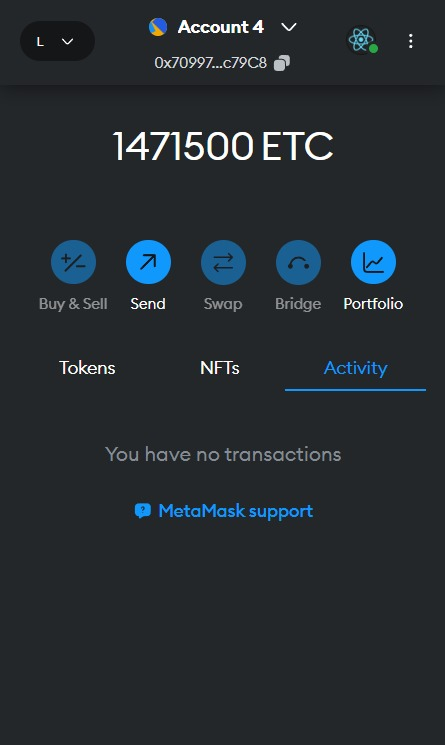
\includegraphics[scale=0.47]{gambar/metamask_akun_2.jpeg}
        % Keterangan gambar yang diinputkan
        \caption{Akun Metamask kedua}
        % Label referensi dari gambar yang diinputkan
        \label{fig:akun2}
        \end{figure}

        \item Pada gambar \ref{fig:makeitem} ketika pengguna memilih untuk membeli sebuah NFT yang ditampilkan pada halaman utama aplikasi, mereka akan mengklik tombol "Buy" yang berada di bawah item yang diinginkan. Langkah ini memicu proses transaksi, di mana Metamask Wallet secara otomatis terbuka, meminta pengguna untuk mengonfirmasi pembelian. Layar Metamask yang muncul merupakan jendela penting yang menampilkan detail transaksi yang harus diperiksa pengguna sebelum mereka melanjutkan. Dalam jendela konfirmasi ini, pengguna akan melihat jumlah total Ethereum (ETH) yang harus dibayarkan, yang sudah termasuk estimasi biaya gas. Biaya gas ini adalah biaya yang dibutuhkan untuk memproses transaksi di jaringan Ethereum, dan nilainya dapat berfluktuasi berdasarkan kepadatan trafik jaringan saat itu. Metamask memberikan dua estimasi: "Estimated fee" yang merupakan perkiraan biaya gas yang akan dikenakan, dan "Max fee" yang menunjukkan batas maksimal biaya yang mungkin ditarik jika kondisi jaringan berubah secara signifikan selama transaksi diproses. Proses ini tidak hanya memindahkan kepemilikan NFT dari penjual ke pembeli, tetapi juga memperbarui semua record yang berkaitan di \emph{blockchain}. Setelah konfirmasi berhasil, NFT akan muncul dalam koleksi pengguna di aplikasi, dan item tersebut akan dihapus dari daftar yang tersedia untuk dijual, menandakan bahwa transaksi telah selesai secara resmi dan NFT kini memiliki pemilik baru. Proses ini menunjukkan integrasi yang mulus antara platform NFT berbasis web dengan teknologi wallet \emph{blockchain} seperti Metamask, menawarkan pengalaman pengguna yang aman dan efisien.
    
      \begin{figure} [H] \centering
        % Nama dari file gambar yang diinputkan
        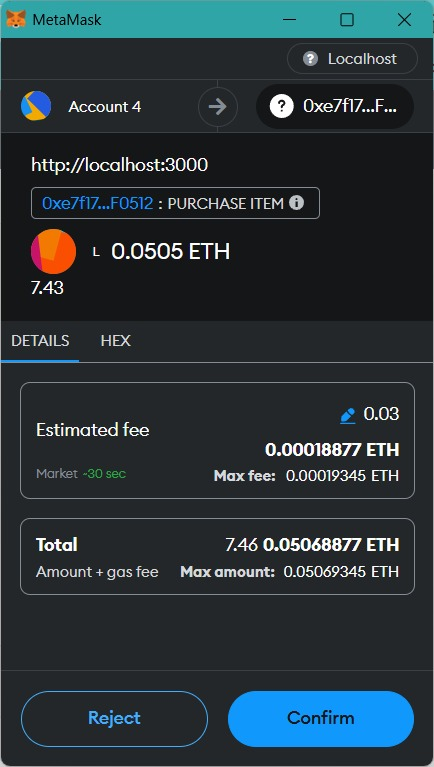
\includegraphics[scale=0.45]{gambar/make_item.jpeg}
        % Keterangan gambar yang diinputkan
        \caption{Proses pembelian NFT}
        % Label referensi dari gambar yang diinputkan
        \label{fig:makeitem}
        \end{figure}
      

    \begin{figure} [H] \centering
    % Nama dari file gambar yang diinputkan
    \frame{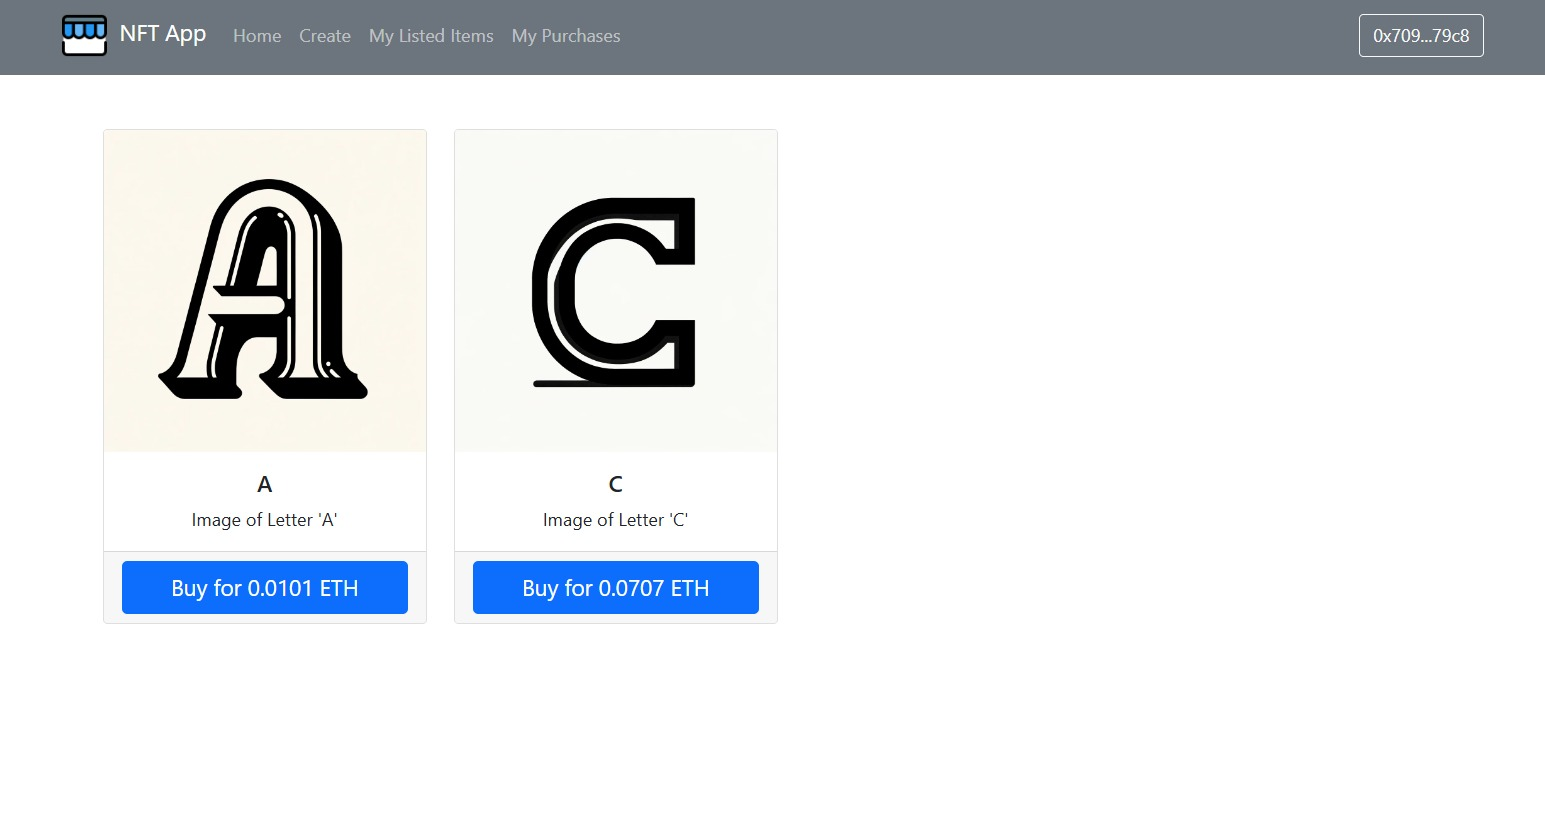
\includegraphics[scale=0.25]{gambar/home_setelah_nft_dibeli.jpg}}
    % Keterangan gambar yang diinputkan
    \caption{Tampilan \emph{home} setelah NFT dibeli}
    % Label referensi dari gambar yang diinputkan
    \label{fig:home_setelah_dibeli}
    \end{figure}
    
    \item Pada gambar \ref{fig:home_setelah_dibeli}, NFT B telah berhasil dibeli oleh \emph{user} B. Proses pembelian ini menyebabkan perubahan langsung pada tampilan halaman \emph{home}, di mana sistem secara otomatis melakukan pembaruan atau \emph{refresh}. Sebelum transaksi, seperti yang terlihat pada gambar \ref{fig:listhome}, ada tiga NFT yang tersedia untuk dibeli. Namun, setelah NFT B dibeli, jumlah NFT yang ditampilkan berkurang menjadi dua. Hal ini menunjukkan bahwa sistem berhasil memperbarui daftar NFT yang tersedia sesuai dengan status penjualan terkini. Proses otomatis ini memastikan bahwa informasi yang disajikan kepada pengguna selalu akurat dan terkini, mencerminkan perubahan real-time pada inventori NFT yang ada dalam platform. Perubahan ini tidak hanya memudahkan pengguna dalam melihat NFT yang masih tersedia tetapi juga meningkatkan pengalaman pengguna dengan menampilkan data yang akurat dan responsif terhadap interaksi pengguna di platform.
    
      \begin{figure} [H] \centering
        % Nama dari file gambar yang diinputkan
        \frame{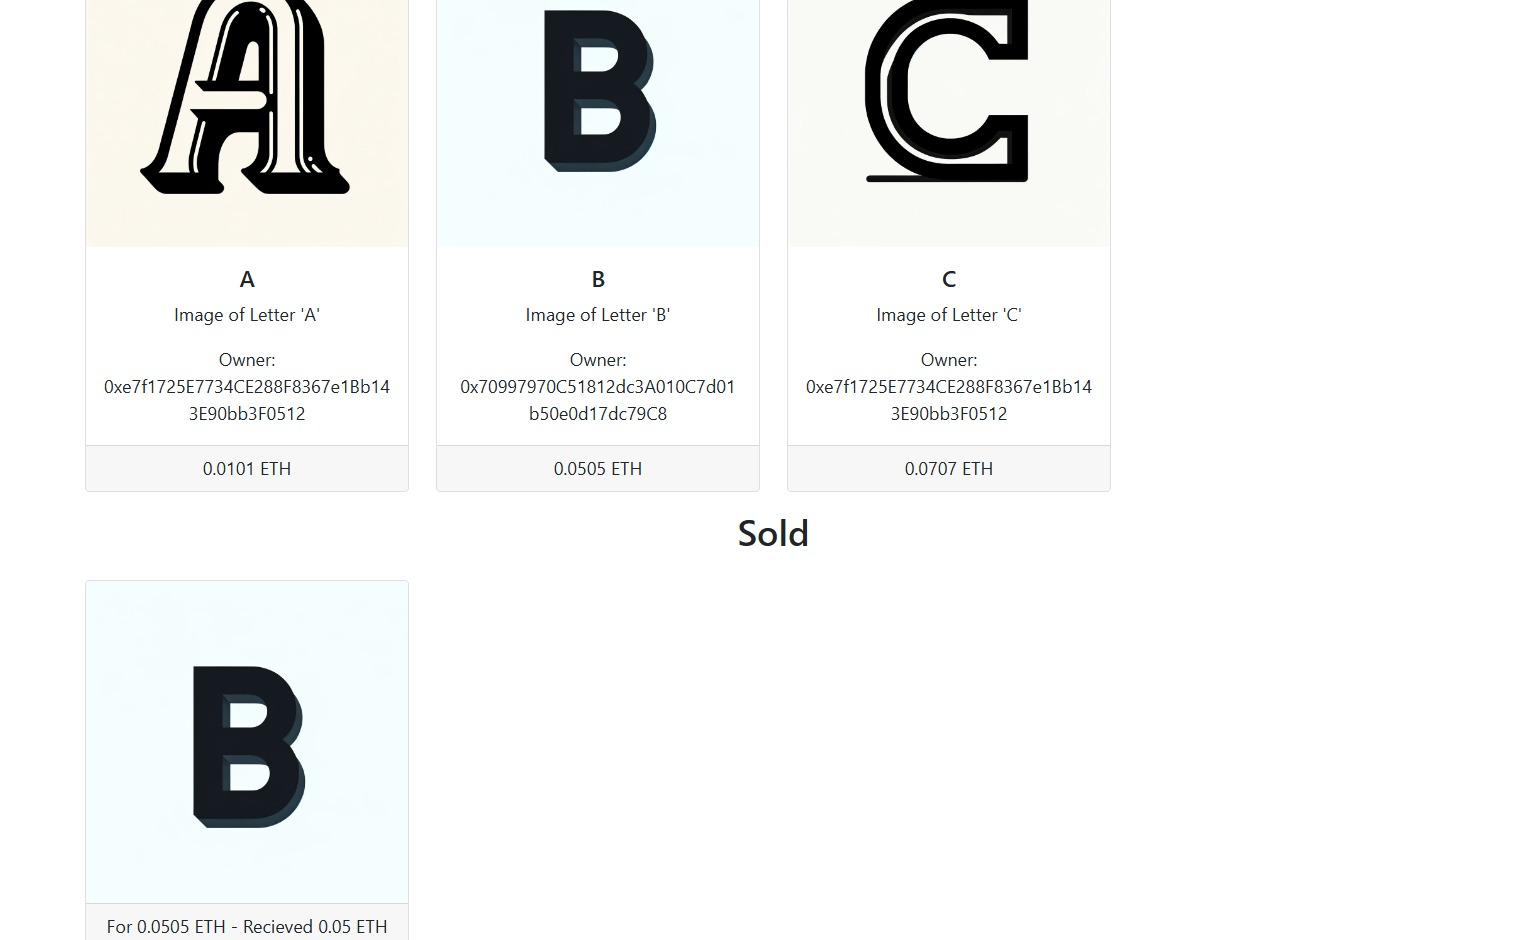
\includegraphics[scale=0.25]{gambar/tampilan_pada_listed_items.jpeg}}
        % Keterangan gambar yang diinputkan
        \caption{Tampilan \emph{Listed items} ketika melakukan pembelian}
        % Label referensi dari gambar yang diinputkan
        \label{fig:new_listed_item}
        \end{figure}

      \item Pada gambar \ref{fig:new_listed_item} di atas, tampilan menunjukkan NFT 'B' yang telah berhasil dibeli oleh pengguna dari akun kedua, sebagaimana terlihat dari pergantian address pemilik ('Owner') pada NFT tersebut dari \emph{address} akun 1 ke alamat \emph{address} dari akun 2. Proses pembelian NFT ini diawali ketika pengguna mengklik tombol pembelian pada salah satu item NFT yang terdaftar di halaman utama, yang kemudian memicu interaksi dengan MetaMask wallet. Pengguna kemudian diminta untuk mengonfirmasi dan menyelesaikan pembayaran melalui wallet tersebut. Setelah transaksi berhasil diverifikasi dan konfirmasi pembayaran diterima, sistem otomatis mengubah status item di halaman "My Listed Items" menjadi "Sold", yang menandakan bahwa item tersebut telah sukses terjual dan tidak lagi tersedia untuk pembelian oleh pengguna lain. Perubahan status ini tidak hanya memastikan transparansi dalam status ketersediaan NFT tetapi juga menunjukkan pembaruan real-time dari kepemilikan aset di platform.
      
      \item Pada gambar \ref{fig:new_listed_item} juga setelah pengguna berhasil menyelesaikan pembelian NFT dari halaman utama, sistem akan memperbarui status NFT tersebut di halaman "My Listed Items" untuk menunjukkan bahwa item telah terjual. Bagian "Sold" di halaman ini akan menampilkan NFT yang telah dibeli, memberikan informasi bahwa NFT tersebut tidak lagi tersedia untuk dibeli oleh pengguna lain. Tampilan ini mencakup gambar NFT, harga jual, serta indikasi bahwa transaksi telah berhasil dengan menunjukkan jumlah ETH yang diterima. Proses ini memastikan bahwa semua pengguna aplikasi dapat melihat secara jelas item yang telah terjual, meningkatkan transparansi dan memudahkan pelacakan kepemilikan NFT. Fungsi ini sangat penting dalam ekosistem NFT, di mana verifikasi kepemilikan dan status penjualan harus diperbarui secara real-time untuk mencegah penjualan ganda dan memastikan integritas platform.
    
      \begin{figure} [H] \centering
        % Nama dari file gambar yang diinputkan
        \frame{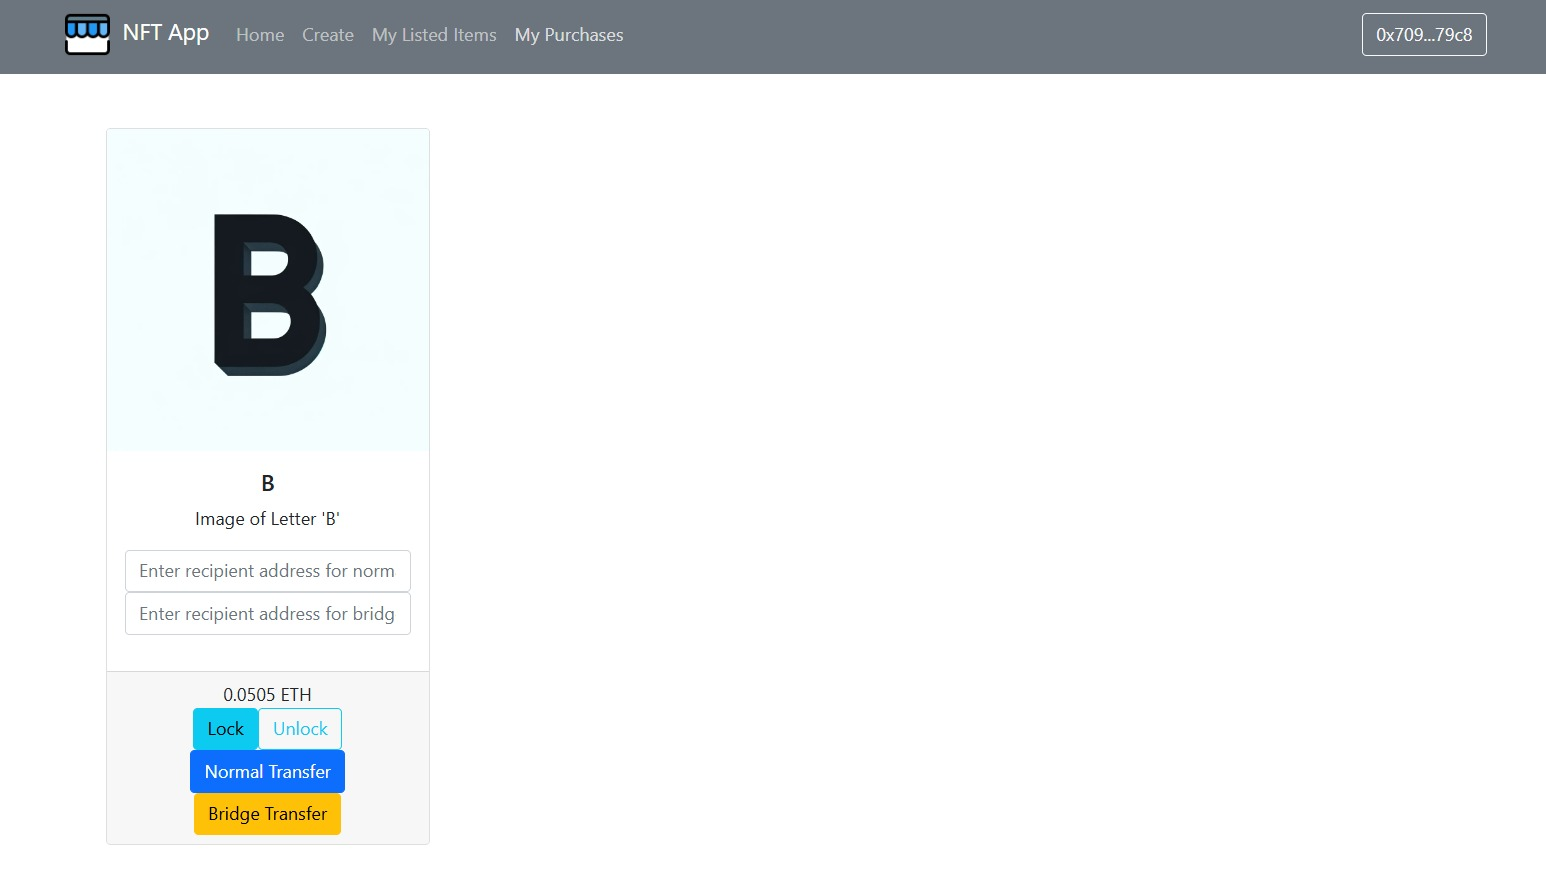
\includegraphics[scale=0.25]{gambar/my_purchases_akun2.jpg}}
        % Keterangan gambar yang diinputkan
        \caption{Tampilan halaman \emph{my purchases} ketika sudah melakukan pembelian}
        % Label referensi dari gambar yang diinputkan
        \label{fig:my_purchases}
        \end{figure}
        \item Lalu pada gambar \ref{fig:my_purchases} adalah tampilan dari halaman \emph{my purchases} di address akun kedua. Pada tampilan ini pemilik dari NFT dapat melihat dari koleksi NFT yang telah dibeli dan juga NFT yang telah dibeli dapat dilakukan hal yaitu \emph{transfer ownership}. \emph{Transfer ownership} yang dapat dilakukan ada dua hal, yaitu \emph{transfer} pada \emph{network} atau \emph{blockchain} yang sama dan juga ada \emph{transfer} pada \emph{network} atau \emph{blockchain} yang berbeda. Kedua fungsi tersebut berbeda karena untuk lintas \emph{blockchain} diperlukan beberapa tahapan atau protokol yaitu terdapat protokol \emph{lock} dan \emph{unlock}. Pada tahapan selanjutnya yang akan dilakukan adalah bagaimana cara melakukan \emph{transfer} dalam satu network yang sama.
        
      \end{itemize}
      
\newpage
\subsection{Pengujian Fitur Transfer \emph{Ownership} Secara \emph{Localhost} Dan Secara Lintas \emph{Blockchain}}

\begin{figure} [H] \centering
  % Nama dari file gambar yang diinputkan
  \frame{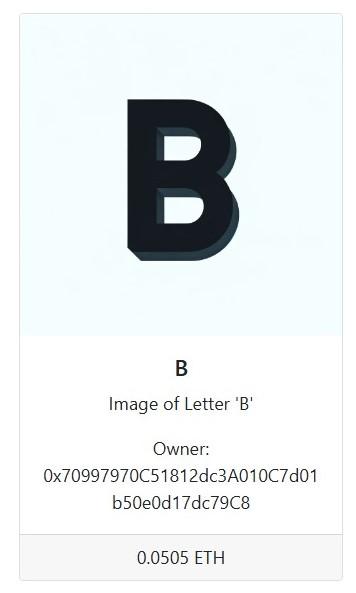
\includegraphics[scale=0.8]{gambar/address_akun_kedua_nft_b.jpeg}}
  % Keterangan gambar yang diinputkan
  \caption{Tampilan halaman \emph{my purchases} ketika sudah melakukan pembelian}
  % Label referensi dari gambar yang diinputkan
  \label{fig:address_nft_b_1}
  \end{figure}

Sebelum melakukan pengujian pemindahan kepemilikan NFT, penggunaan akun ketiga dengan \emph{address} "0x3C44CdDdB6a900fa2b585dd299e03d12FA4293BC" sangat krusial. Akun ini secara khusus disiapkan untuk menangani proses transfer kepemilikan NFT dari akun kedua. Seperti yang terlihat pada gambar \ref*{fig:listeditem}, awalnya NFT diunggah melalui halaman \emph{create} dan secara otomatis, \emph{owner} pertama NFT adalah \emph{address} dari \emph{smart contract} yang melakukan \emph{minting}. Hal ini berubah setelah NFT dibeli, sebagaimana ditunjukkan dalam gambar \ref{fig:address_nft_b_1} di mana \emph{address} akun kedua menjadi pemilik baru. Perpindahan kepemilikan ini terjadi melalui transaksi yang tercatat dan diverifikasi dalam blockchain, memastikan bahwa NFT berpindah tangan dari akun pencipta ke pembeli dengan aman dan terdokumentasi dengan jelas, menunjukkan kekuatan dan fleksibilitas teknologi \emph{smart contract} dalam mengelola aset digital dalam ekosistem blockchain.

\begin{figure} [H] \centering
  % Nama dari file gambar yang diinputkan
  \frame{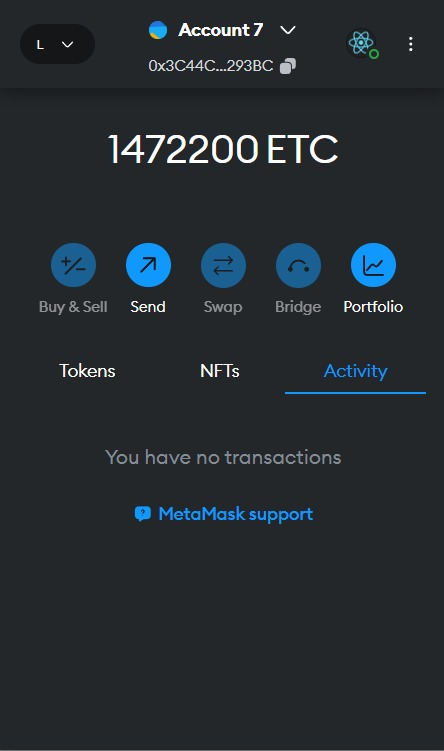
\includegraphics[scale=0.4]{gambar/metamask_akun_3.jpg}}
  % Keterangan gambar yang diinputkan
  \caption{Detail akun ketiga pada Metamask Wallet}
  % Label referensi dari gambar yang diinputkan
  \label{fig:detail_akun_3}
  \end{figure}

Pada gambar \ref*{fig:detail_akun_3}, terlihat tampilan akun MetaMask yang disebut "Account 7" dengan saldo yang menonjol sebanyak 1472200 ETC, yang menunjukkan jumlah Ethereum Classic di dalam wallet. Akun ini, yang beralamat di 0x3C44CdDdB6a900fa2b585dd299e03d12FA4293
BC, belum memiliki catatan transaksi apapun, menandakan bahwa belum ada aktivitas jual beli, pengiriman, penukaran, atau transaksi lainnya yang dilakukan. Hal ini juga memperlihatkan bahwa akun ini adalah akun baru atau belum digunakan untuk transaksi. Akun ini didapatkan dari kunci privat yang berasal dari node Hardhat, sering digunakan dalam pengembangan dan pengujian smart contract di lingkungan lokal. Akun ini direncanakan akan digunakan sebagai penerima dalam proses transfer kepemilikan NFT, memanfaatkan fasilitas yang disediakan MetaMask untuk mengelola aset kripto dan interaksi dengan \emph{blockchain}.

Ekspektasi dari pengujian fitur \emph{transfer ownership} pada web3.0 yang telah dibuat lain adalah sebagai berikut:
\begin{itemize}
    \item Pengguna dari pemilik NFT yang sekarang (pengguna \emph{address} kedua) dapat melakukan pemindahan kepemilikan NFT yang telah dimiliki menjadi kepemilikan pengguna \emph{address} ketiga yang berada dalam \emph{network} yang sama yaitu \emph{localhost}.

    \item Pengguna dari pemilik NFT yang sekarang (pengguna pertama) dapat melakukan pemindahan kepemilikan NFT yang telah dimiliki menjadi kepemilikan pengguna pengguna kedua berada dalam \emph{network} yang berbeda yaitu \emph{Sepolia Testnet} pada pengguna pertama dan \emph{BNB Chain Testnet} pada pengguna kedua.

    \item Pada halaman \emph{my listed item} pembuat dar NFT awal (pengguna \emph{address} pertama) \emph{owner} dari NFT yang telah dilakukan \emph{transfer ownership} secara \emph{localhost} maupun lintas \emph{blockchain} itu alamatnya berganti dari \emph{address} pemilik lama menjadi \emph{address} pemilik baru. 
    
\end{itemize}

Berikut ini merupakan langkah pengujian beserta dengan pembahasan dari pengujian fitur transfer \emph{ownership} Secara \emph{Localhost} Dan Secara Lintas \emph{Blockchain}:

\begin{itemize}
  \item Pada gambar \ref*{fig:my_purchases}, dapat dilihat pada halaman \emph{my purchases} milik \emph{address} akun kedua terdapat NFT "B".  Setelah transaksi pembelian NFT ini, platform menyediakan opsi untuk mengelola NFT tersebut, termasuk kemampuan untuk melakukan transfer kepemilikan atau memblokirnya untuk transaksi lebih lanjut. Pengguna dapat memasukkan alamat penerima untuk transfer normal atau transfer lintas rantai, memanfaatkan fungsionalitas yang memudahkan transfer NFT antara berbagai blockchain atau dalam jaringan yang sama.
  
  \begin{figure} [H] \centering
    % Nama dari file gambar yang diinputkan
    \frame{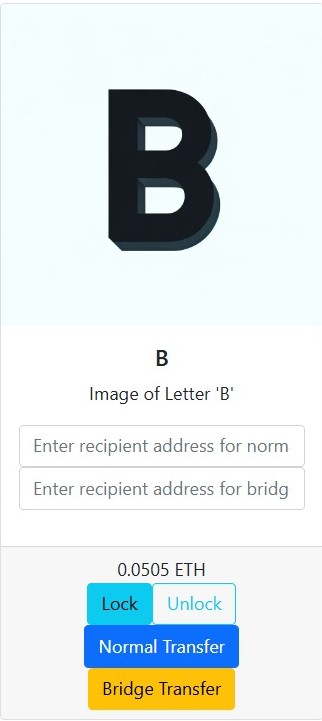
\includegraphics[scale=0.6]{gambar/normal_transfer.jpg}}
    % Keterangan gambar yang diinputkan
    \caption{Tampilan NFT yang siap dilakukan pindah kepemilikan}
    % Label referensi dari gambar yang diinputkan
    \label{fig:normal_transfer}
    \end{figure}

  \item Pada pengujian ini, digunakan NFT "B" yang akan dilakukan transfer \emph{ownership} dalam satu \emph{network}, pada kolom pertama yang bertuliskan "Enter recipient address for normal transfer \emph{ownership}" akan dimasukkan \emph{address} dari akun ketiga yang berupa "\emph{0x3C44CdD dB6a900fa2b585dd299e03d12FA4293BC}". Setelah dimasukkan \emph{address} tersebut maka akan langsung saja ditekannya tombol "\emph{Normal Transfer}". Tombol "\emph{Normal Transfer}" tersebut lalu akan membuat pengguna langsung membuka window dari Metamask Wallet untuk melakukan transaksi pembayaran dari "\emph{gas}" atau fee yang harus dibayarkan setiap kali kode dari \emph{smart contract} tereksekusi. Setiap aksi yang dilakukan oleh \emph{smart contract} seperti transaksi, perubahan data, atau eksekusi fungsi—memerlukan gas tertentu.
  
  \begin{figure} [H] \centering
  % Nama dari file gambar yang diinputkan
  \frame{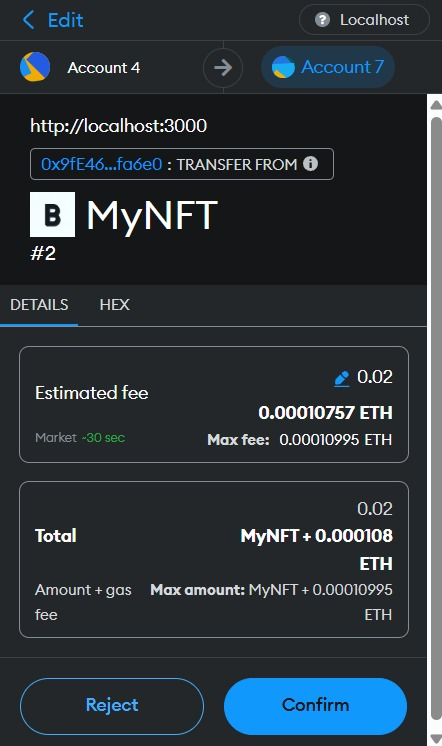
\includegraphics[scale=0.45]{gambar/my_nft_b.jpg}}
  % Keterangan gambar yang diinputkan
  \caption{Tampilan NFT yang siap dilakukan pindah kepemilikan}
  % Label referensi dari gambar yang diinputkan
  \label{fig:nft_b}
  \end{figure}
  
  \item Gambar \ref*{fig:nft_b} ini menunjukkan tampilan antarmuka Metamask saat pengguna kedua siap melakukan transaksi transfer dari NFT bernama "MyNFT" dengan nomor \#2. Nomor \#2 ditunjukkan bahwa NFT itu memiliki indeks urutan kedua. Pada tampilan ini, pengguna diberi informasi mengenai jumlah ETH yang akan ditransfer sebesar 0.02 ETH dan biaya transaksi yang diperkirakan. Biaya ini terbagi menjadi dua, yaitu biaya perkiraan (estimated fee) sebesar 0.00010757 ETH dan biaya maksimal (\emph{max fee}) sebesar 0.00010995 ETH, yang memberikan kejelasan tentang berapa banyak gas yang mungkin diperlukan untuk menyelesaikan transaksi tersebut dalam waktu kurang lebih 30 detik. Fitur ini memfasilitasi pengguna dalam memastikan bahwa mereka memiliki cukup saldo untuk menutupi biaya transaksi saat melakukan transfer NFT. Tampilan juga menawarkan pilihan untuk menyetujui atau menolak transaksi yang akan dilakukan.
  
  \begin{figure} [H] \centering
  % Nama dari file gambar yang diinputkan
  \frame{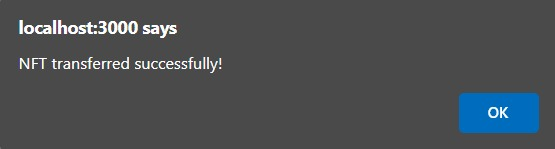
\includegraphics[scale=0.70]{gambar/transfer_berhasil.jpg}}
  % Keterangan gambar yang diinputkan
  \caption{\emph{Alert} "\emph{NFT transferred successfully!}" ketika NFT berhasil dipindahkan}
  % Label referensi dari gambar yang diinputkan
  \label{fig:alert}
  \end{figure}

  \item Setelah pengguna melakukan konfirmasi transaksi pada Metamask Wallet seperti pada gambar \ref*{fig:normal_transfer} dan transaksi berhasil, maka akan muncul \emph{alert} berupa "\emph{NFT transferred successfully!}".
  
  \begin{figure} [H] \centering
    % Nama dari file gambar yang diinputkan
    \frame{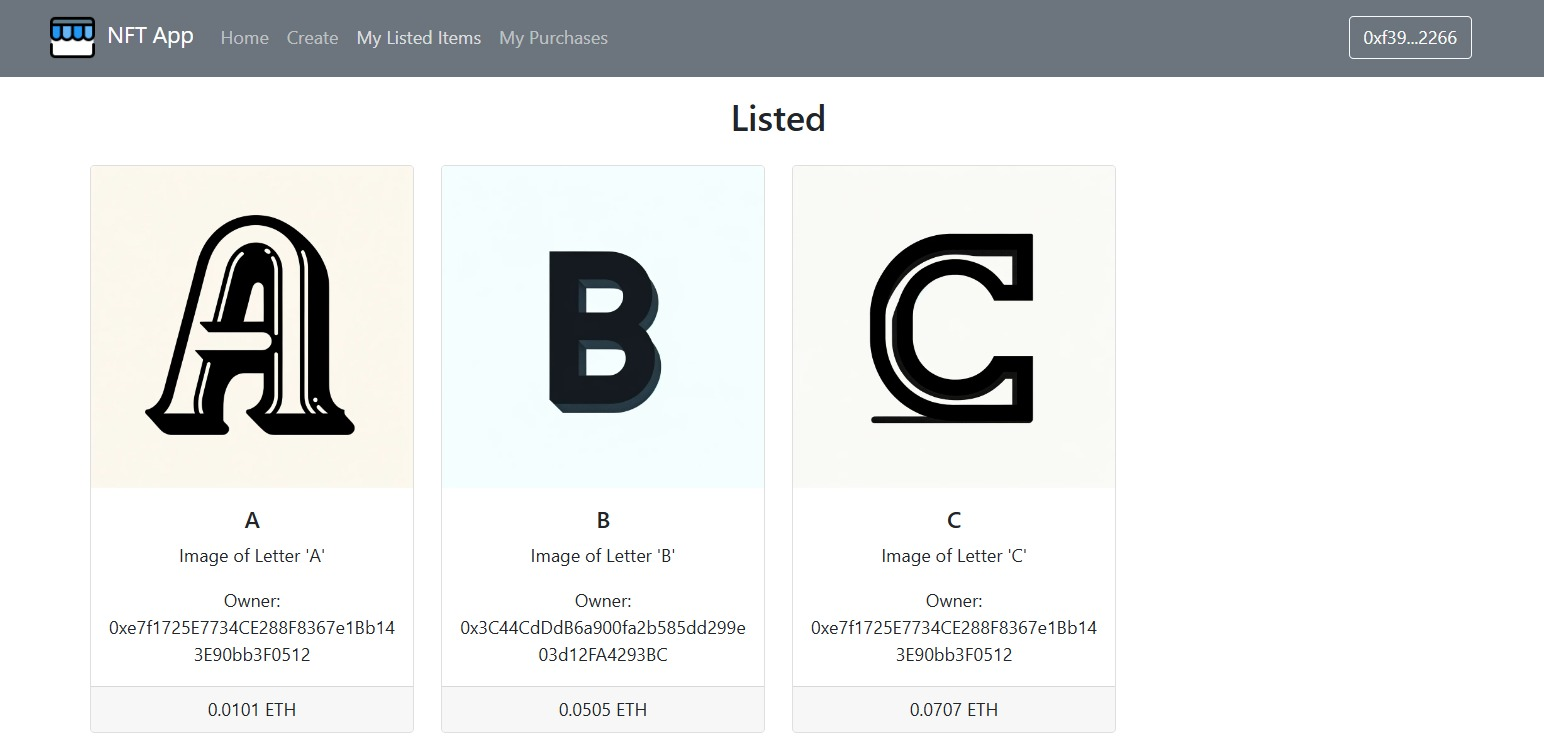
\includegraphics[scale=0.25]{gambar/letter_b_to_akun3.jpg}}
    % Keterangan gambar yang diinputkan
    \caption{\emph{Alert} "\emph{NFT transferred successfully!}" ketika NFT berhasil dipindahkan}
    % Label referensi dari gambar yang diinputkan
    \label{fig:letter_b_akun3}
    \end{figure}

  \item Dapat dilihat pada gambar \ref*{fig:letter_b_akun3} pada halaman \emph{my listed items} milik pengguna \emph{address} pertama yang me-\emph{minting} NFT B, jika dibandingkan dengan gambar \ref*{fig:address_nft_b_1}, \emph{owner} dari NFT B telah berganti menjadi \emph{address} milik akun ketiga. Ini membuktikan bahwa NFT B kepemilikannya berhasil dipindahkan dari \emph{address} pengguna kedua menjadi \emph{address} pengguna ketiga.

  \begin{figure} [H] \centering
    % Nama dari file gambar yang diinputkan
    \frame{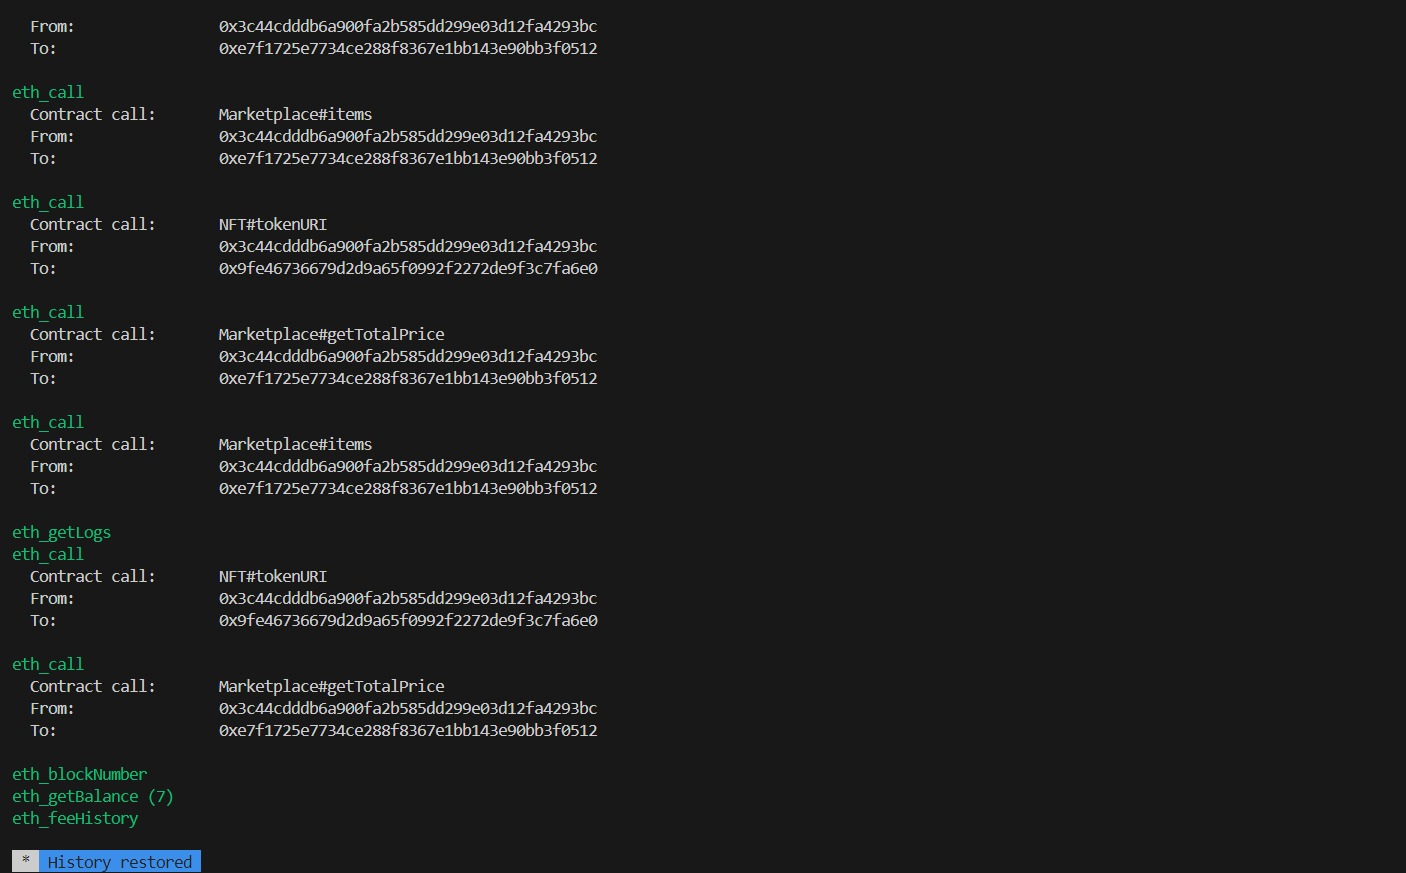
\includegraphics[scale=0.27]{gambar/hardhat_transaction.jpg}}
    % Keterangan gambar yang diinputkan
    \caption{Console Transaksi Pada \emph{Hardhat Node}}
    % Label referensi dari gambar yang diinputkan
    \label{fig:hardhat}
    \end{figure}

    \item Pada gambar \ref*{fig:hardhat} adalah detail transaksi yang terjadi pada \emph{smart contract} ketika ada fungsi yang tersekekusi. Dikarenakan pengembangan web3.0 dan juga sistem \emph{smart contract} ini dilakukan secara lokal, maka \emph{contract call} dan juga detail dari \emph{hash block} hanya dapat dilihat pada \emph{node} yang berada pada EVM milik Hardhat.
    
    \begin{figure} [H] \centering
      % Nama dari file gambar yang diinputkan
      \frame{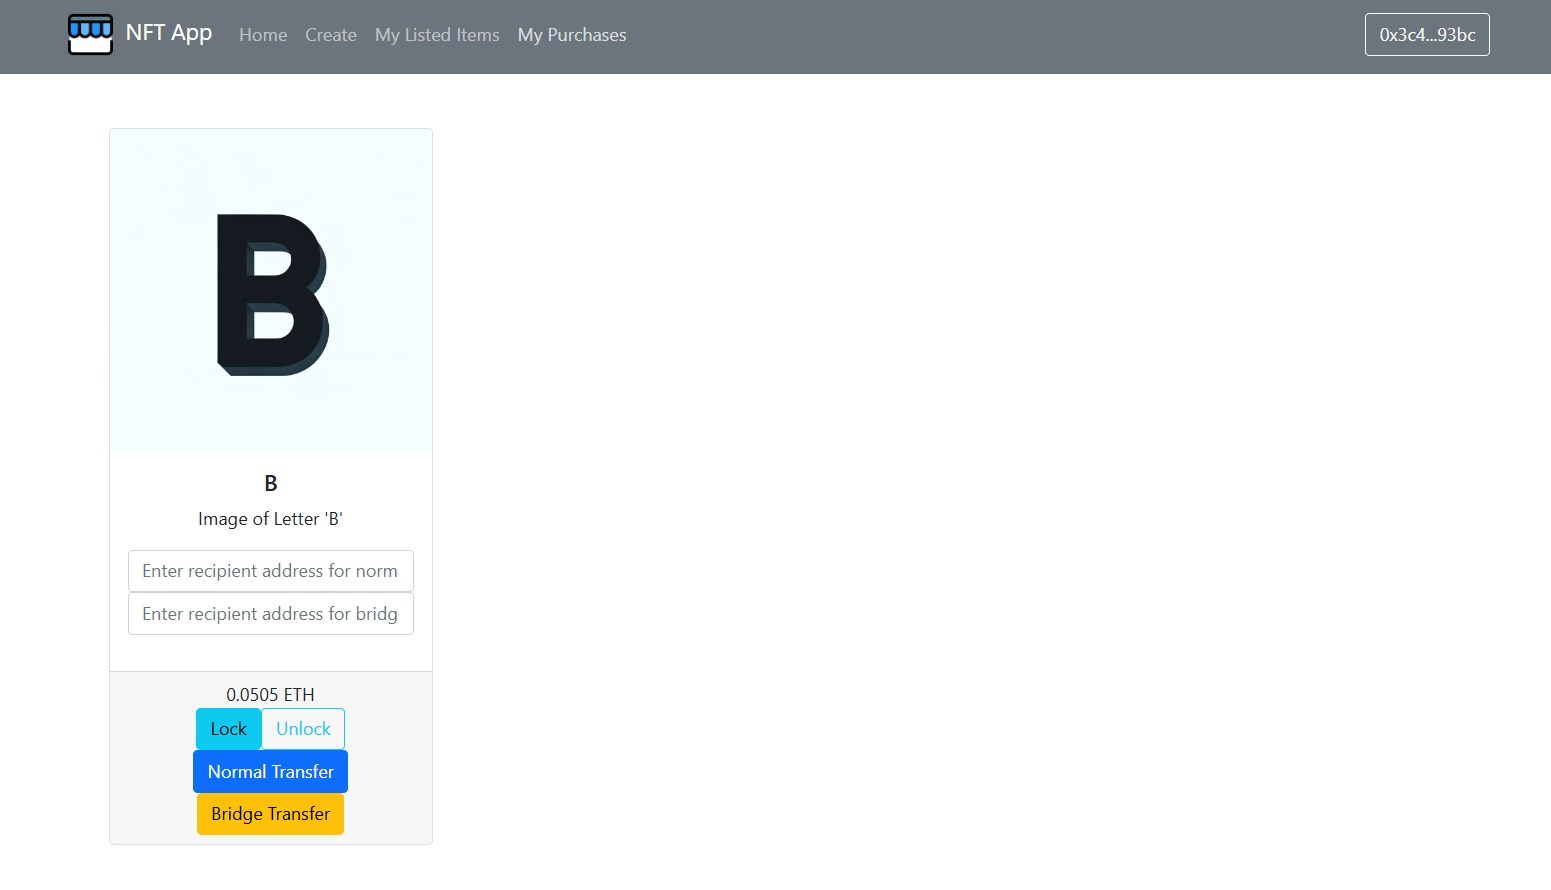
\includegraphics[scale=0.27]{gambar/letter_b_akun3.jpg}}
      % Keterangan gambar yang diinputkan
      \caption{Tampilan halaman \emph{my purchases} pada akun ketiga}
      % Label referensi dari gambar yang diinputkan
      \label{fig:akunketiga}
      \end{figure}

    \item Lalu selain dari \ref*{fig:letter_b_akun3} juga terdapat hasil bahwa NFT telah berpindah pada akun ketiga. Hal ini dapat dilihat pada \emph{box} kanan atas menunjukkan \emph{address} dari akun ketiga yang berarti ini adalah halaman \emph{my purchases} milik akun ketiga. Lalu akun ketiga ini juga yang memiliki wewenang penuh dalam kepemilikan NFT yang sebelumnya dimiliki oleh akun kedua.
    
    \begin{figure} [H] \centering
      \centering
      \begin{subfigure}{0.45\textwidth}
          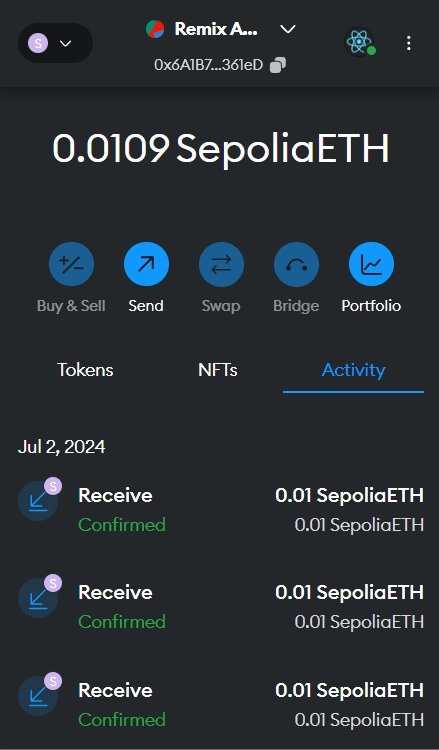
\includegraphics[scale=0.32]{gambar/sepolia_akun.jpg}
          \caption{}
          \label{fig:sepolia}
      \end{subfigure}
      \hspace{5pt}
      \begin{subfigure}{0.45\textwidth}
        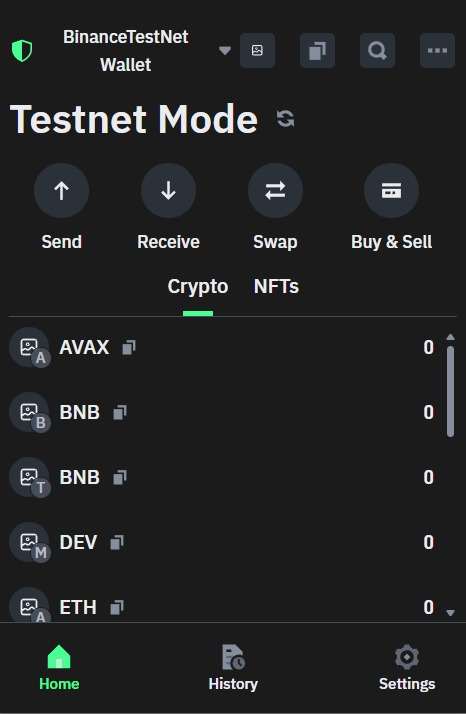
\includegraphics[scale=0.32]{gambar/btc_akun.jpg}
        \caption{}
        \label{fig:binance}
    \end{subfigure}
      \caption{Detail Akun Untuk Pengujian Lintas Rantai}
      \label{fig:detail_akun}
      \end{figure}

    \item Gambar pertama menggambarkan akun di Sepolia Ethereum Testnet dengan saldo SepoliaETH yang ditampilkan secara jelas. Ini termasuk aktivitas terkini yang mencakup penerimaan SepoliaETH, memperlihatkan aktivitas yang dikonfirmasi dalam jaringan. Akun pada gambar pertama ini akan digunakan sebagai \emph{address} penerima dari NFT yang dikirimkan dari \emph{network} yang berbeda. Akun ini memiliki \emph{address} "0x6A1B77e82b61D54C4
    F1A27cd00A27325EBf361eD"
    
    \item Gambar kedua menampilkan BinanceTestNet Wallet dalam mode testnet, yang memungkinkan pengguna untuk mengirim, menerima, bertukar, dan membeli aset kripto seperti AVAX, BNB, DEV, dan ETH dalam lingkungan tes. Akun pada gambar kedua ini akan digunakan sebagai \emph{address} penerima dari NFT yang dikirimkan dari \emph{network} yang berbeda. Akun ini memiliki \emph{address} "0xD066d6576D9485Eb2c2a41BB8B52EcE17a0557d6"
    
    \begin{figure} [H] \centering
      % Nama dari file gambar yang diinputkan
      \frame{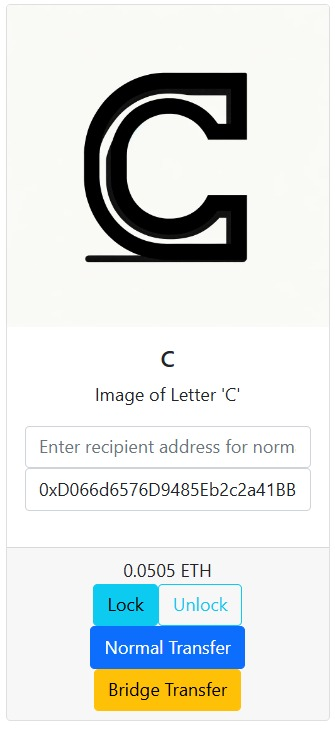
\includegraphics[scale=0.5]{gambar/interoperability_1.jpg}}
      % Keterangan gambar yang diinputkan
      \caption{Memasukkan \emph{address} tujuan untuk \emph{bridge transfer}}
      % Label referensi dari gambar yang diinputkan
      \label{fig:bridge_transfer}
      \end{figure}

    \item Pengujian untuk melakukan tes interoperabilitas atau transfer \emph{ownership} lintas \emph{blockchain} dilakukan dengan prosedur yang terstruktur. Pertama, akun pengirim yang beroperasi di jaringan \emph{localhost} akan memilih NFT yang ingin ditransfer. Kemudian, alamat tujuan dari akun yang berjalan di jaringan Sepolia diisi ke dalam sistem. Proses transfer diawali dengan penguncian (\emph{lock}) NFT untuk memastikan keamanan selama transisi. Fungsi \emph{lock} ini penting untuk mencegah transaksi atau interaksi lain yang mungkin mempengaruhi NFT selama proses transfer belum selesai. Setelah NFT terkunci, barulah transfer ownership akan dijalankan melalui fungsi \emph{bridge transfer}.
    
    \begin{figure} [H] \centering
      % Nama dari file gambar yang diinputkan
      \frame{\includegraphics[scale=0.4]{gambar/fungsi_lock.jpg}}
      % Keterangan gambar yang diinputkan
      \caption{Konfirmasi pembayaran gas dari fungsi \emph{lock token} di Metamask Wallet}
      % Label referensi dari gambar yang diinputkan
      \label{fig:lock_token}
      \end{figure}
    
    \item Setelah melakukan konfirmasi pembayaran gas dari fungsi \emph{lock} token, kondisi NFT berubah menjadi \emph{locked}. Setelah NFT menjadi \emph{locked} maka NFT sudah aman untuk dilakukan transaksi lintas \emph{blockchain}. 
    
    \begin{figure} [H] \centering
      % Nama dari file gambar yang diinputkan
      \frame{\includegraphics[scale=0.4]{gambar/bridge.jpg}}
      % Keterangan gambar yang diinputkan
      \caption{Konfirmasi pembayaran gas dari fungsi \emph{bridge} transfer di Metamask Wallet}
      % Label referensi dari gambar yang diinputkan
      \label{fig:bridge_transfer}
      \end{figure}
    
      \item Setelah melakukan konfirmasi pembayaran gas dari fungsi \emph{bridge} transfer, kepemilikan dari NFT "C" berpindah dari akun pertama yang memiliki \emph{address} "0xf39Fd6e51aad88F6
      F4ce6aB8827279cffFb92266" yang berjalan pada \emph{network localhost} menjadi kepemilikan akun yang berjalan pada \emph{network BNB Smart Chain} dengan alamat "0xD066d657
      6D9485Eb2c2a41BB8B52EcE17a0557d6". Hal ini dapat dibuktikan pada gambar di bawah ini.

      \begin{figure} [H] \centering
        % Nama dari file gambar yang diinputkan
        \frame{\includegraphics[scale=0.45]{gambar/smart_chain.jpg}}
        % Keterangan gambar yang diinputkan
        \caption{Kepemilikan NFT "C" Berganti Menjadi Akun \emph{Network BNB Smart Chain}}
        % Label referensi dari gambar yang diinputkan
        \label{fig:bridge_transfer}
        \end{figure}
      
      \item Kemudian hal yang perlu dilakukan yang terakhir adalah mengubah \emph{state} dari NFT tersebut yang awalnya "\emph{locked}" menjadi "\emph{unlocked}". Hal ini harus dilakukan agar NFT tersebut dapat digunakan untuk transaksi lagi pada \emph{network} tersebut.
      
      \begin{figure} [H] \centering
        % Nama dari file gambar yang diinputkan
        \frame{\includegraphics[scale=0.4]{gambar/unlock_token.jpg}}
        % Keterangan gambar yang diinputkan
        \caption{Konfirmasi Pembayaran Gas \emph{Unlock} Token}
        % Label referensi dari gambar yang diinputkan
        \label{fig:unlock_token}
        \end{figure}
      
    \item Setelah melakukan penguncian NFT, langkah berikutnya adalah membuka kunci atau "unlock" NFT tersebut agar dapat kembali digunakan dalam transaksi. Proses ini melibatkan interaksi dengan sistem \emph{blockchain} yang tercatat sebagai transaksi dengan estimasi biaya yang diperlihatkan dalam gambar. Di sini, biaya transaksi atau '\emph{gas fee}' yang diperkirakan untuk membuka kunci token ditampilkan, menekankan pentingnya memperhatikan biaya transaksi yang harus dibayar untuk memproses kegiatan ini di \emph{blockchain}. Proses membuka kunci ini tidak hanya mengizinkan pemilik untuk memindahkan atau menjual NFT tersebut, tetapi juga penting untuk memastikan fleksibilitas dan likuiditas NFT di pasar.
    
    \begin{figure} [H] \centering
    % Nama dari file gambar yang diinputkan
    \frame{\includegraphics[scale=0.4]{gambar/interoperabilitas_2.jpg}}
    % Keterangan gambar yang diinputkan
    \caption{Hasil Akhir Dari Transfer Lintas Rantai}
    % Label referensi dari gambar yang diinputkan
    \label{fig:lintas_rantai}
    \end{figure}

    \item Setelah dilakukan pengujian yang sama tetapi memasukkan \emph{address} dari akun yang berada pada \emph{network sepolia ethereum}, untuk transfer \emph{ownership} NFT B dapat dilihat di gambar \ref*{fig:lintas_rantai} kepemilikan atau \emph{owner} dari NFT B juga berubah menjadi \emph{address} dari akun \emph{sepolia}. 
    
    \begin{figure} [H] \centering
      % Nama dari file gambar yang diinputkan
      \frame{\includegraphics[scale=0.7]{gambar/block_hash.jpg}}
      % Keterangan gambar yang diinputkan
      \caption{\emph{Block Hash} dari setiap transaksi}
      % Label referensi dari gambar yang diinputkan
      \label{fig:hash_block}
      \end{figure}

    \item Pada gambar \ref*{fig:hash_block}, merupakan \emph{block hash} dari transaksi yang telah terjadi. \emph{Hash Blocks} ini didapatkan dari Hardhat. \emph{Block hash} adalah nilai unik yang dihasilkan dari \emph{blok} data dalam \emph{blockchain}, yang bertindak sebagai identitas digital \emph{blok} tersebut. Hash ini dihasilkan menggunakan algoritma hash kriptografi, yang mengubah informasi \emph{blok} menjadi string karakter tetap panjang yang kompleks dan unik. Proses ini memastikan keamanan dan integritas data dalam \emph{blockchain} karena setiap perubahan kecil pada \emph{blok} akan menghasilkan hash yang sangat berbeda, sehingga mudah untuk mendeteksi perubahan atau manipulasi data. Hash \emph{blok} juga digunakan untuk menghubungkan \emph{blok}-\emph{blok} dalam \emph{blockchain} \emph{hash} dari \emph{blok} sebelumnya dimasukkan ke dalam \emph{blok} berikutnya, menciptakan rantai data yang terkait dan aman.
\end{itemize}
\cleardoublepage

% Bab 5 penutup
\chapter{PENUTUP}
\label{chap:penutup}

% Ubah bagian-bagian berikut dengan isi dari penutup

\section{Kesimpulan}
\label{sec:kesimpulan}

Dalam penelitian ini, penulis telah mengeksplorasi dan mengimplementasikan konsep interoperabilitas NFT berbasis blockchain menggunakan smart contract dalam konteks Web3.0. Studi ini berhasil menunjukkan potensi dan efektivitas teknologi blockchain, khususnya Ethereum, dalam mendukung penciptaan dan pengelolaan NFT yang dapat beroperasi lintas berbagai token. Lalu Kesimpulan dari penelitian ini adalah
\begin{itemize}
\item Implementasi Smart contract yang dirancang telah berhasil memfasilitasi penciptaan, transaksi, dan verifikasi NFT secara aman dan efisien. Dengan menggunakan standar ERC-721, penulis telah mengimplementasikan NFT yang unik dan dapat dilacak asal-usulnya, yang sangat penting dalam ekosistem Web3.0.
\item NFT yang dikembangkan menunjukkan interoperabilitas lintas berbagai platform \emph{blockchain} Hal ini dicapai melalui penggunaan protokol \emph{cross-chain interoperability protocol} yang konsisten.
\end{itemize}

\section{Saran}
Untuk meningkatkan interoperabilitas dan efisiensi penggunaan NFT d disarankan agar penelitian lebih lanjut difokuskan pada pengembangan protokol yang lebih universal untuk integrasi lintas rantai. Selain itu, penelitian lebih lanjut diperlukan untuk menyempurnakan mekanisme keamanan yang dapat melindungi privasi pengguna sambil mempertahankan transparansi dan keandalan sistem blockchain.
\cleardoublepage

\chapter*{DAFTAR PUSTAKA}
\addcontentsline{toc}{chapter}{DAFTAR PUSTAKA}
\renewcommand\refname{}
\vspace{2ex}
\renewcommand{\bibname}{}
\begingroup
\def\chapter*#1{}
\printbibliography
\endgroup
\cleardoublepage

% Biografi penulis
\begin{center}
  \Large
  \textbf{BIOGRAFI PENULIS}
\end{center}

\addcontentsline{toc}{chapter}{BIOGRAFI PENULIS}

\vspace{2ex}

\begin{wrapfigure}{L}{0.3\textwidth}
  \centering
  \vspace{-3ex}
  % Ubah file gambar berikut dengan file foto dari mahasiswa
  \includegraphics[width=0.3\textwidth]{gambar/foto_biografi.jpg}
  \vspace{-4ex}
\end{wrapfigure}

% Ubah kalimat berikut dengan biografi dari mahasiswa
\name{}, lahir di kota Tulungagung pada 24 Maret 2002, adalah seorang mahasiswa yang memiliki kecintaan mendalam terhadap teknologi dan inovasi. Saat ini, Arya menempuh pendidikan di Institut Teknologi Sepuluh Nopember, di jurusan Teknik Komputer, yang dikenal dengan keunggulan akademis dan kontribusinya dalam teknologi informasi.

Di luar kelas, Arya mengejar berbagai hobi yang memperkaya wawasan dan keterampilannya, seperti mendengarkan musik, membaca buku, dan yang terutama adalah mengeksplorasi kemajuan terbaru dalam teknologi. Kecintaannya terhadap musik dan buku membuka perspektif baru dan menambah kedalaman pemahamannya tentang dunia.

Arya telah terlibat dalam sejumlah proyek yang menunjukkan keahliannya dalam pengembangan backend menggunakan Node.js, serta pengalaman dalam DevOps dan cloud computing dengan menggunakan platform Google Cloud. Keahliannya tidak terhenti di situ; ia juga mengembangkan kemampuan dalam bidang machine learning dan robotic operating system, yang menunjukkan keberanian dan kecakapan teknisnya dalam menghadapi tantangan baru.

Lebih lanjut, Arya juga mendalami pengembangan frontend menggunakan React JS, mengintegrasikan desain yang responsif dengan pengalaman pengguna yang intuitif. Terbaru, ia mulai mengeksplorasi ranah blockchain dan smart contract dengan menggunakan Solidity, menandai langkah selanjutnya dalam perjalanan teknologinya.

Dengan basis pengetahuan yang luas dan terus berkembang, Arya berambisi untuk menjadi inovator dan pemimpin di dunia teknologi, menggunakan setiap proyek dan kesempatan pembelajaran sebagai batu loncatan menuju keberhasilan yang lebih besar.

\cleardoublepage

\end{document}
